\chapter{Eredmények}
\label{ch:results}

\section{Vizsgált kódbázisok}

Egy kódbázisnak a következő feltételeket kell teljesíteni, hogy vizsgálni tudjuk:
\begin{enumerate}
    \item Legyen könnyen build-elhető, évekre visszamenően
    \item A tesztek legyenek könnyen futtathatóak
    \item Generálódjon coverage report a teszt futtatásokhoz és a report formátuma legyen egyike azoknak, amiket támogat a ReportGenerator\footnote{https://github.com/danielpalme/ReportGenerator} nevű .NET-es könyvtár
    \item A projekt legyen nyílt forráskódú
    \item Rendelkezzen a projekt viszonylag gazdag commit történettel -- jelen esetben az 5000+ commit és 3+ éves történet heurisztikát alkalmaztam
\end{enumerate}

Ezeket a feltételeket ugyan könnyű teljesíteni egy fejlesztő csapatnak ipari környezetben saját projektekre, sajnos nyílt forráskódú környezetben más a helyzet -- specifikusan az 1-es és 3-as pontok jelentenek problémát. A C++-ra, Python-ra és .NET Framework-re épülő projektek például egy az egyben kiesnek, mert egyik sem ad egyszerű módot arra, hogy a build-eléshez szükséges környezetet könnyen elő tudjuk állítani a projekt életciklusának akármely pontján.

Gyakorlatban a JavaScript NodeJS/NPM, .NET Core/.NET 5+ és Java ökoszisztémákra épülő projektek felelhetnek meg a korábbi feltételeknek. Ezek közül azonban a Java a szakmai hátterem miatt kiesik, a .NET Core/5+ projektek jelentős többsége pedig az 5-ös feltételt nem teljesíteni, így marad a JavaScript Node/NPM ökoszisztéma. A specifikus projekteknél külön meg fogom említeni, de általánosságban itt is leírom: még a JavaScript/NodeJS/NPM ökoszisztéma esetén is komoly problémát jelent a régi (~2015 előtti) verziók build-elése, mivel az NPM és a node, illetve a rájuk épített projektek sok változáson estek át az évek során, amit ma a projekt ismerete nélkül már nehéz reprodukálni. Ez azt jelenti, hogy a legtöbb esetben lehetetlen

Fontos leszögezni még egy dolgot. A JavaScript-es projektek elemzése egy jelentős vakfoltot fog képezni, méghozzá azért, mert a nyílt forráskódú projektek között gyakorlatilag lehetetlen olyat találni, amire őszintén azt lehet mondani, hogy rossz minőségű kódbázissal rendelkezik. Nyilván egy kódbázis minősége szubjektív, de a GitHub-on host-olt JavaScript projektek túlnyomó többsége 95\% feletti coverage-el rendelkezik. Ráadásul azok a projektek, amik 95\% alatt vannak, azok jellemzően csak a nagyon konzervatív coverage ignore path-ok miatt mutatnak ilyen értékeket -- a React projekt például 80\% körüli értéket mutatott, azonban hamar kiderült, hogy ez csak azért van, mert halott kódot tartanak a repository-ban, amit már nem hajtanak meg unit tesztek.

A fentieket figyelembe véve a következő projektekre esett a választás:
\begin{itemize}
    \item Vue: https://github.com/vuejs/vue
    \item Express: https://github.com/expressjs/express
    \item React: https://github.com/facebook/react
    \item Gatsby: https://github.com/gatsbyjs/gatsby
\end{itemize}

\section{Vue}

Elsőként a vue.js\footnote{\url{https://github.com/vuejs/vue}} kódbázisát fogjuk megvizsgálni. A Vue egy progresszív, JavaScript-alapú frontend framework. A Vue feature-ök tekintetében valahol a másik két nagy frontend framework, az Angular és a React között van -- nem próbál egy kikövezett utat adni, mint az Angular, de nem csak egy specifikus szeletét fedi le a frontend fejlesztésnek, mint a React.

\lstset{language=HTML, caption={Egy egyszerű Vue komponens}}
\begin{lstlisting}
<div id="app">
    {{ message }}
</div>
\end{lstlisting}

\lstset{language=JavaScript, caption={Egy egyszerű Vue komponens JS kódja}}
\begin{lstlisting}
var app = new Vue({
    el: '#app',
    data: {
        message: 'Hello Vue!'
    }
})
\end{lstlisting}

A projekt viszonylag fiatal, a fejlesztése 2016-ban kezdődött. A későbbi megfigyelések szempontjából érdemes megjegyezni, hogy ugyan jelen pillanatban 338 egyedi kontribútora van a projektnek, a fejlesztés nagy része egy fejlesztőhöz, Evan You nevéhez köthető:

\lstset{caption={A vue.js top 10 kontribútora}}
\begin{lstlisting}
vue git:(dev) git shortlog -sn | head -n10
    2303  Evan You
    78  vue-bot
    47  Hanks
    34  Eduardo San Martin Morote
    32  kazuya kawaguchi
    30  chengchao
    25  katashin
    21  AchillesJ
    18  Herrington Darkholme
    15  JK
\end{lstlisting}\label{code:vue-authors}

Az analízist a vue esetében az első publikus release-től kezdjük.

\subsection{Vue 1.0}

A vue több szempontból is különös eset lesz: egyrészt az első publikus release-ig gyakorlatilag egy egyszemélyes projekt volt, másrészt pedig, ahogy azt később látni fogjuk, a Vue 2.0 egy teljes újraírása volt a projektnek.

Először vessünk egy pillantást a \ref{table:vue1-top-files} táblázatra, amiben a vue 1.0-ás változatának legtöbbet módosított fájljai láthatóak. Látható, hogy bár egy fejlesztője van a projektnek és 100\%-os coverage-el rendelkezik, már itt kialakulóban van fájloknak egy halmaza, amik vonzani fogják magukhoz a későbbi változtatásokat és javításokat. A \code{compile.js}, \code{directive.js} és \code{watcher.js} fájlokra kiemelten érdemes figyelni, mert ezek már most kiemelkednek az átlagból méret és változtatások száma tekintetében (átlag fájl méret 147, átlag változtatások száma 20 a teljes repository-ra).

\begin{table}[h]
    \centering
    \begin{tabular}{l|l|l|l|l}
        Filename      & Lifetime Authors & Lifetime Changes & Line Count & Coverage \% \\ \hline
        compile.js    & 2                & 123              & 709        & 100         \\
        directive.js  & 1                & 102              & 320        & 100         \\
        init.js       & 1                & 80               & 114        & 100         \\
        watcher.js    & 3                & 72               & 344        & 100         \\
        vue.js        & 1                & 52               & 96         & 100         \\
        lifecycle.js  & 1                & 49               & 68         & 100         \\
        data.js       & 1                & 45               & 174        & 100         \\
        lang.js       & 4                & 44               & 388        & 100         \\
        dom.js        & 2                & 42               & 362        & 100         \\
        transclude.js & 2                & 40               & 148        & 100         \\
        global.js     & 1                & 39               & 152        & 100
    \end{tabular}
    \caption{A vue 1.0-ás kiadásának leggyakrabban módosított fájljai} \label{table:vue1-top-files}
\end{table}

Érdekes továbbá a változtatások számáról készített hisztogram a \ref{fig:vue1-hist} ábrán, amiről jól látszik, hogy a 67 forrás fájlból álló vue 1.0 változtatásainak egy jelentős része 5 fájl köré csoportosul, amik méret és változtatás szám szepontjából már most az átlag többszörösét mutatják.

\begin{figure}[h]
    \centering
    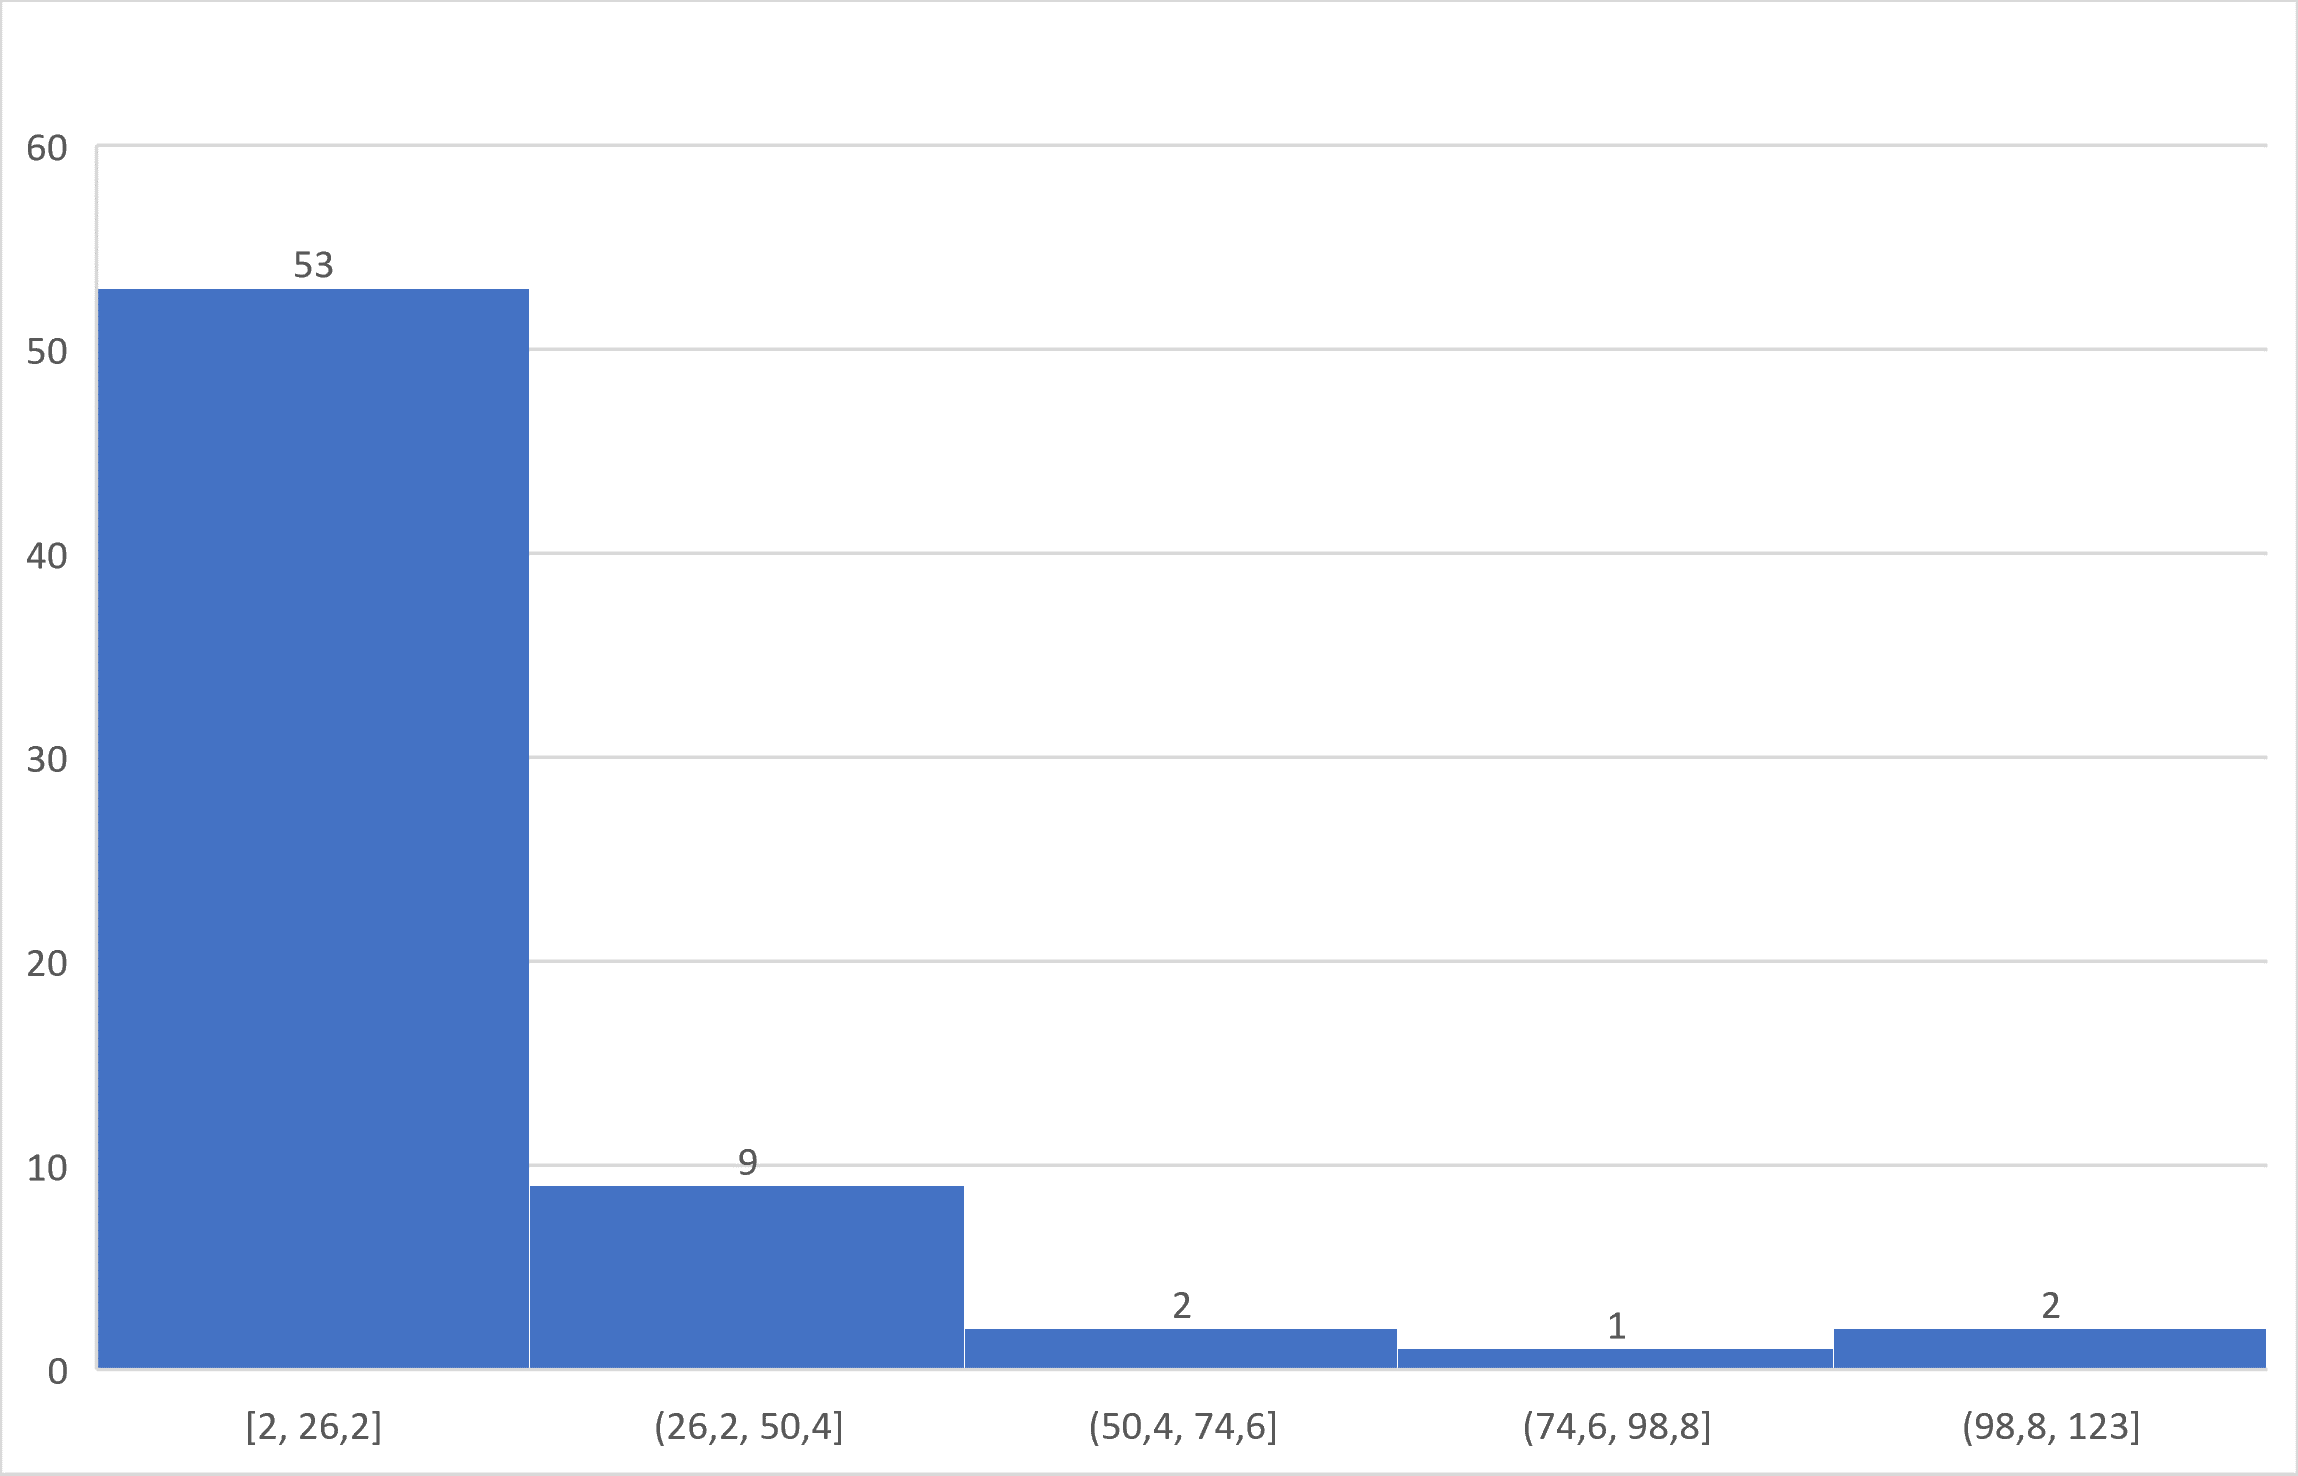
\includegraphics[width=1\textwidth]{images/vue/vue1-hist.png}
    \caption{Fájlonkénti változtatások számának a hisztogramja}
    \label{fig:vue1-hist}
\end{figure}

A \ref{fig:vue1-cov-changes} ábra mutatja a teljes repository-n a fájlonkénti változtatások számát csökkenő sorrendben, illetve a másodlagos tengelyen látható a fájlonkénti coverage. A coverage egyelőre 100\% a teljes projekten. A változtatások számára illesztett görbét érdemes megjegyezni, mert visszatérő motívum lesz a többi analízis során is.

A \ref{fig:vue1-changes-lines} az egyéni fájlok változtatási számát és a fájlok méretét ábrázolja. Bár van néhány fájl, mint például a \code{vue.js} és a \code{directive.js}, amik a sok változtatás ellenére kis méretűek, a kódbázis nagy részére igaz, hogy minél több módosítás tartozik egy fájlhoz, annál nagyobb -- számszerűsítve a korreláció a két adatsor között 0,59 a vue 1.0 esetében.

\begin{figure}[H]
    \centering
    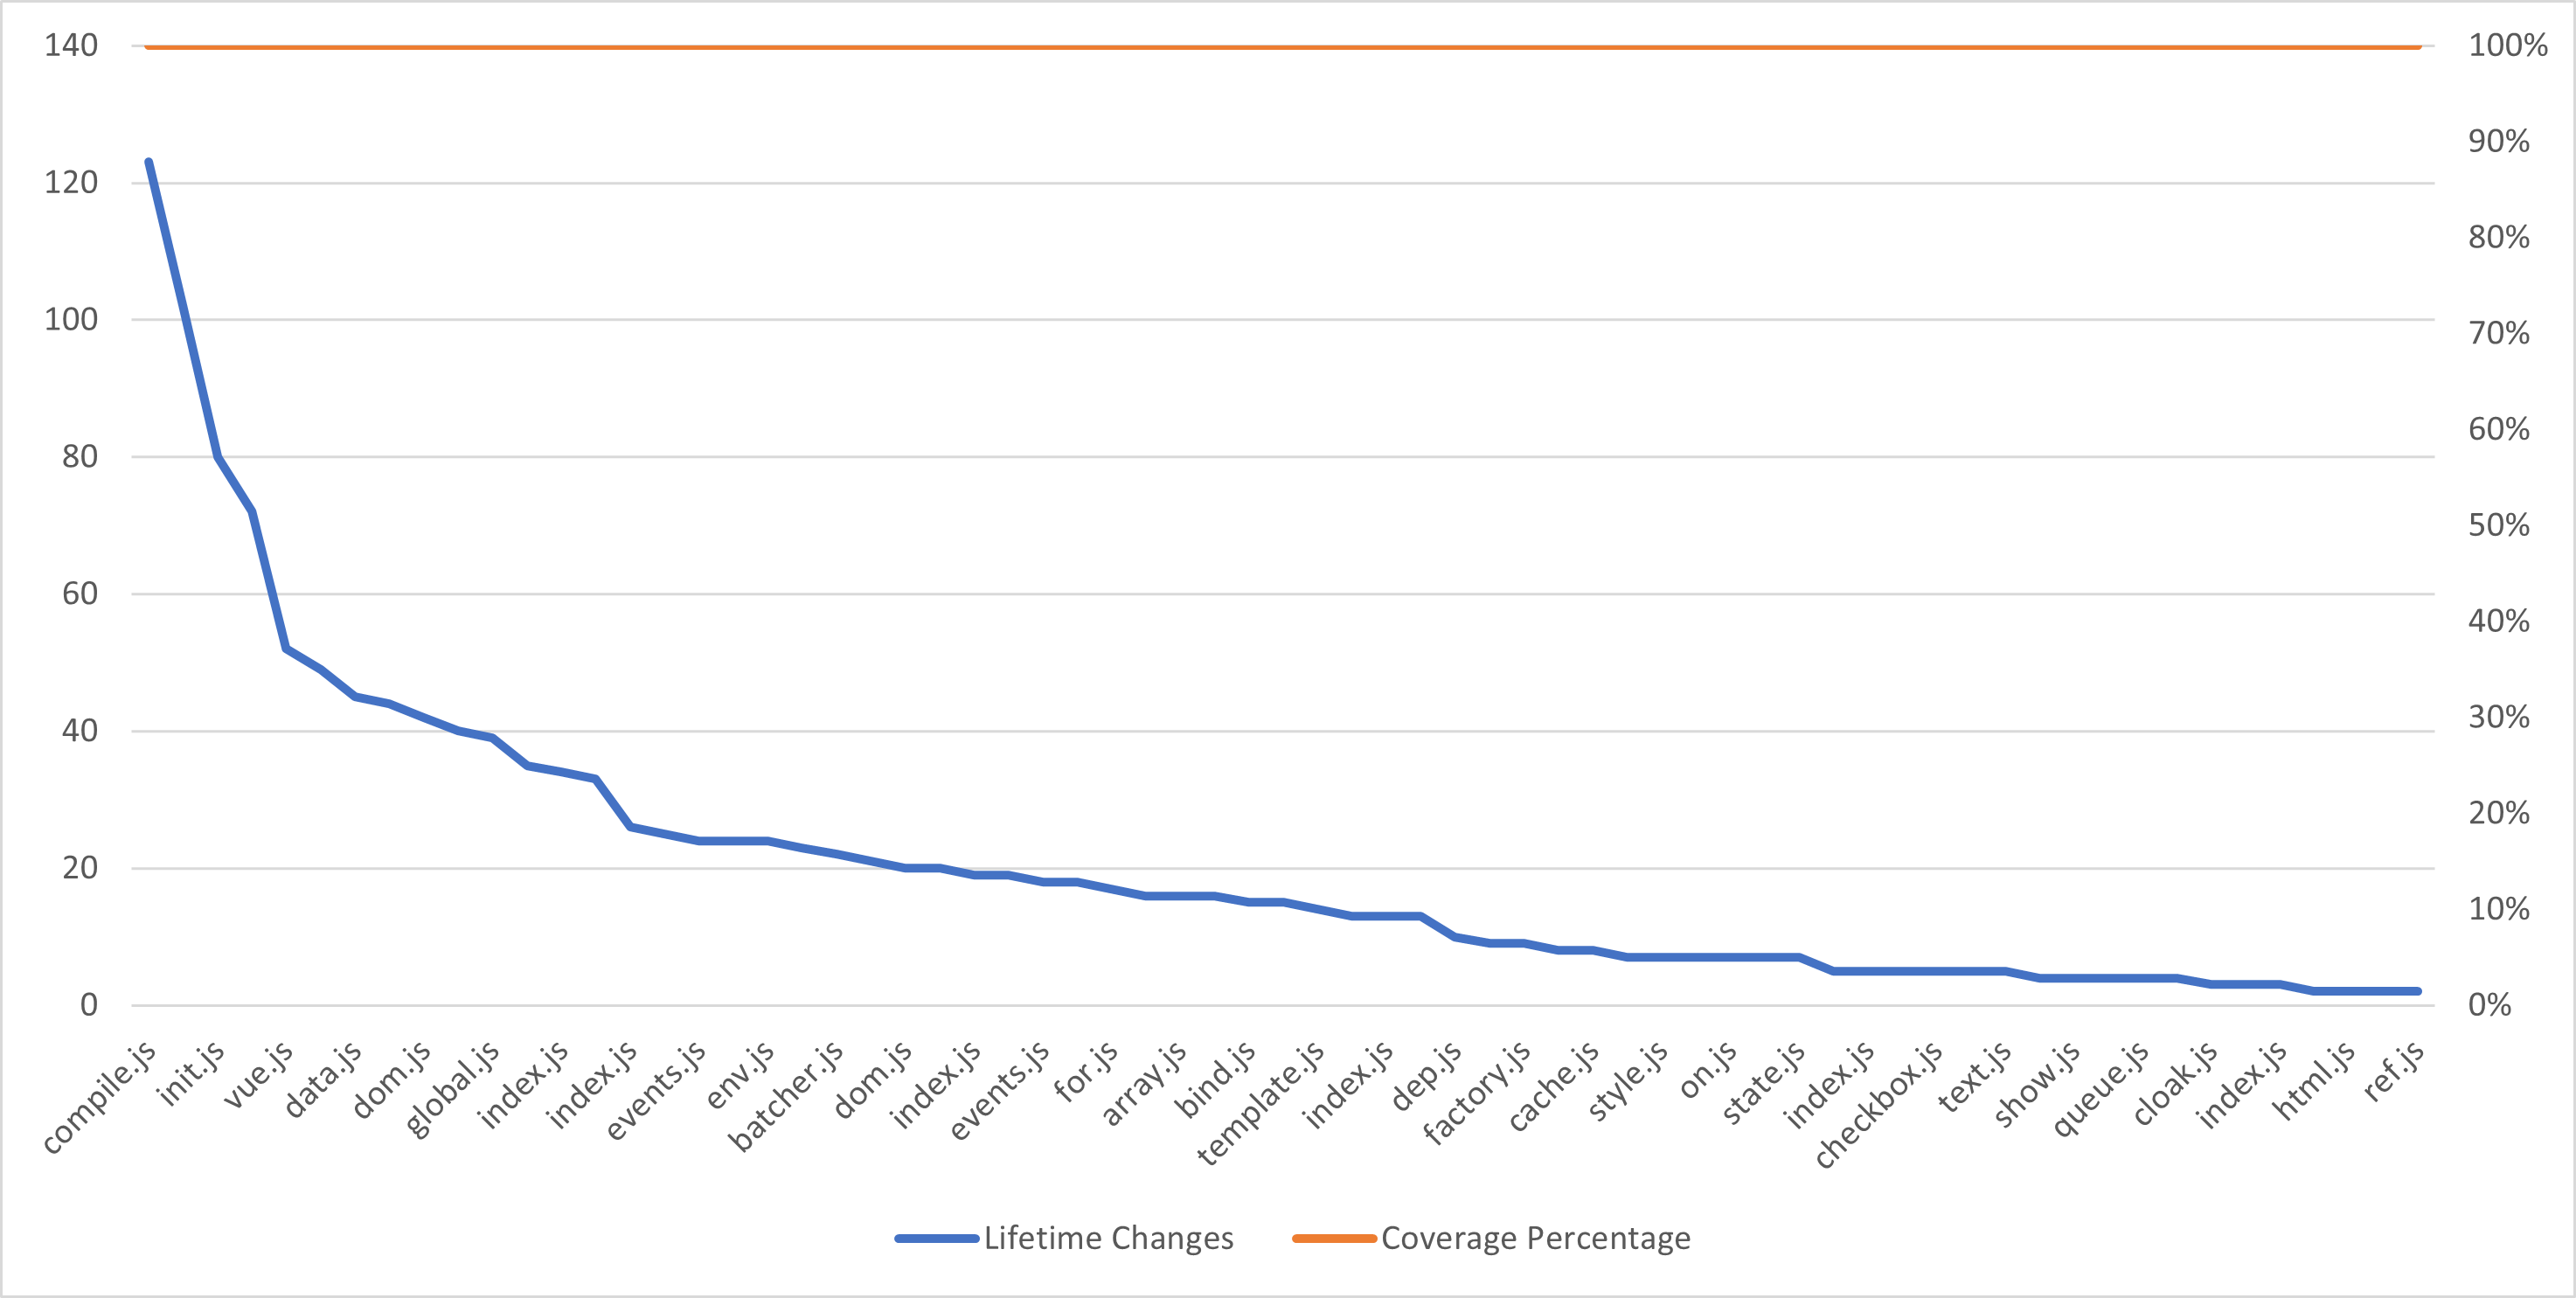
\includegraphics[width=1\textwidth]{images/vue/vue1-lifetime-changes.png}
    \caption{A coverage és az összes változtatások számának alakulása a vue 1.0 esetében}
    \label{fig:vue1-cov-changes}
\end{figure}

\begin{figure}[H]
    \centering
    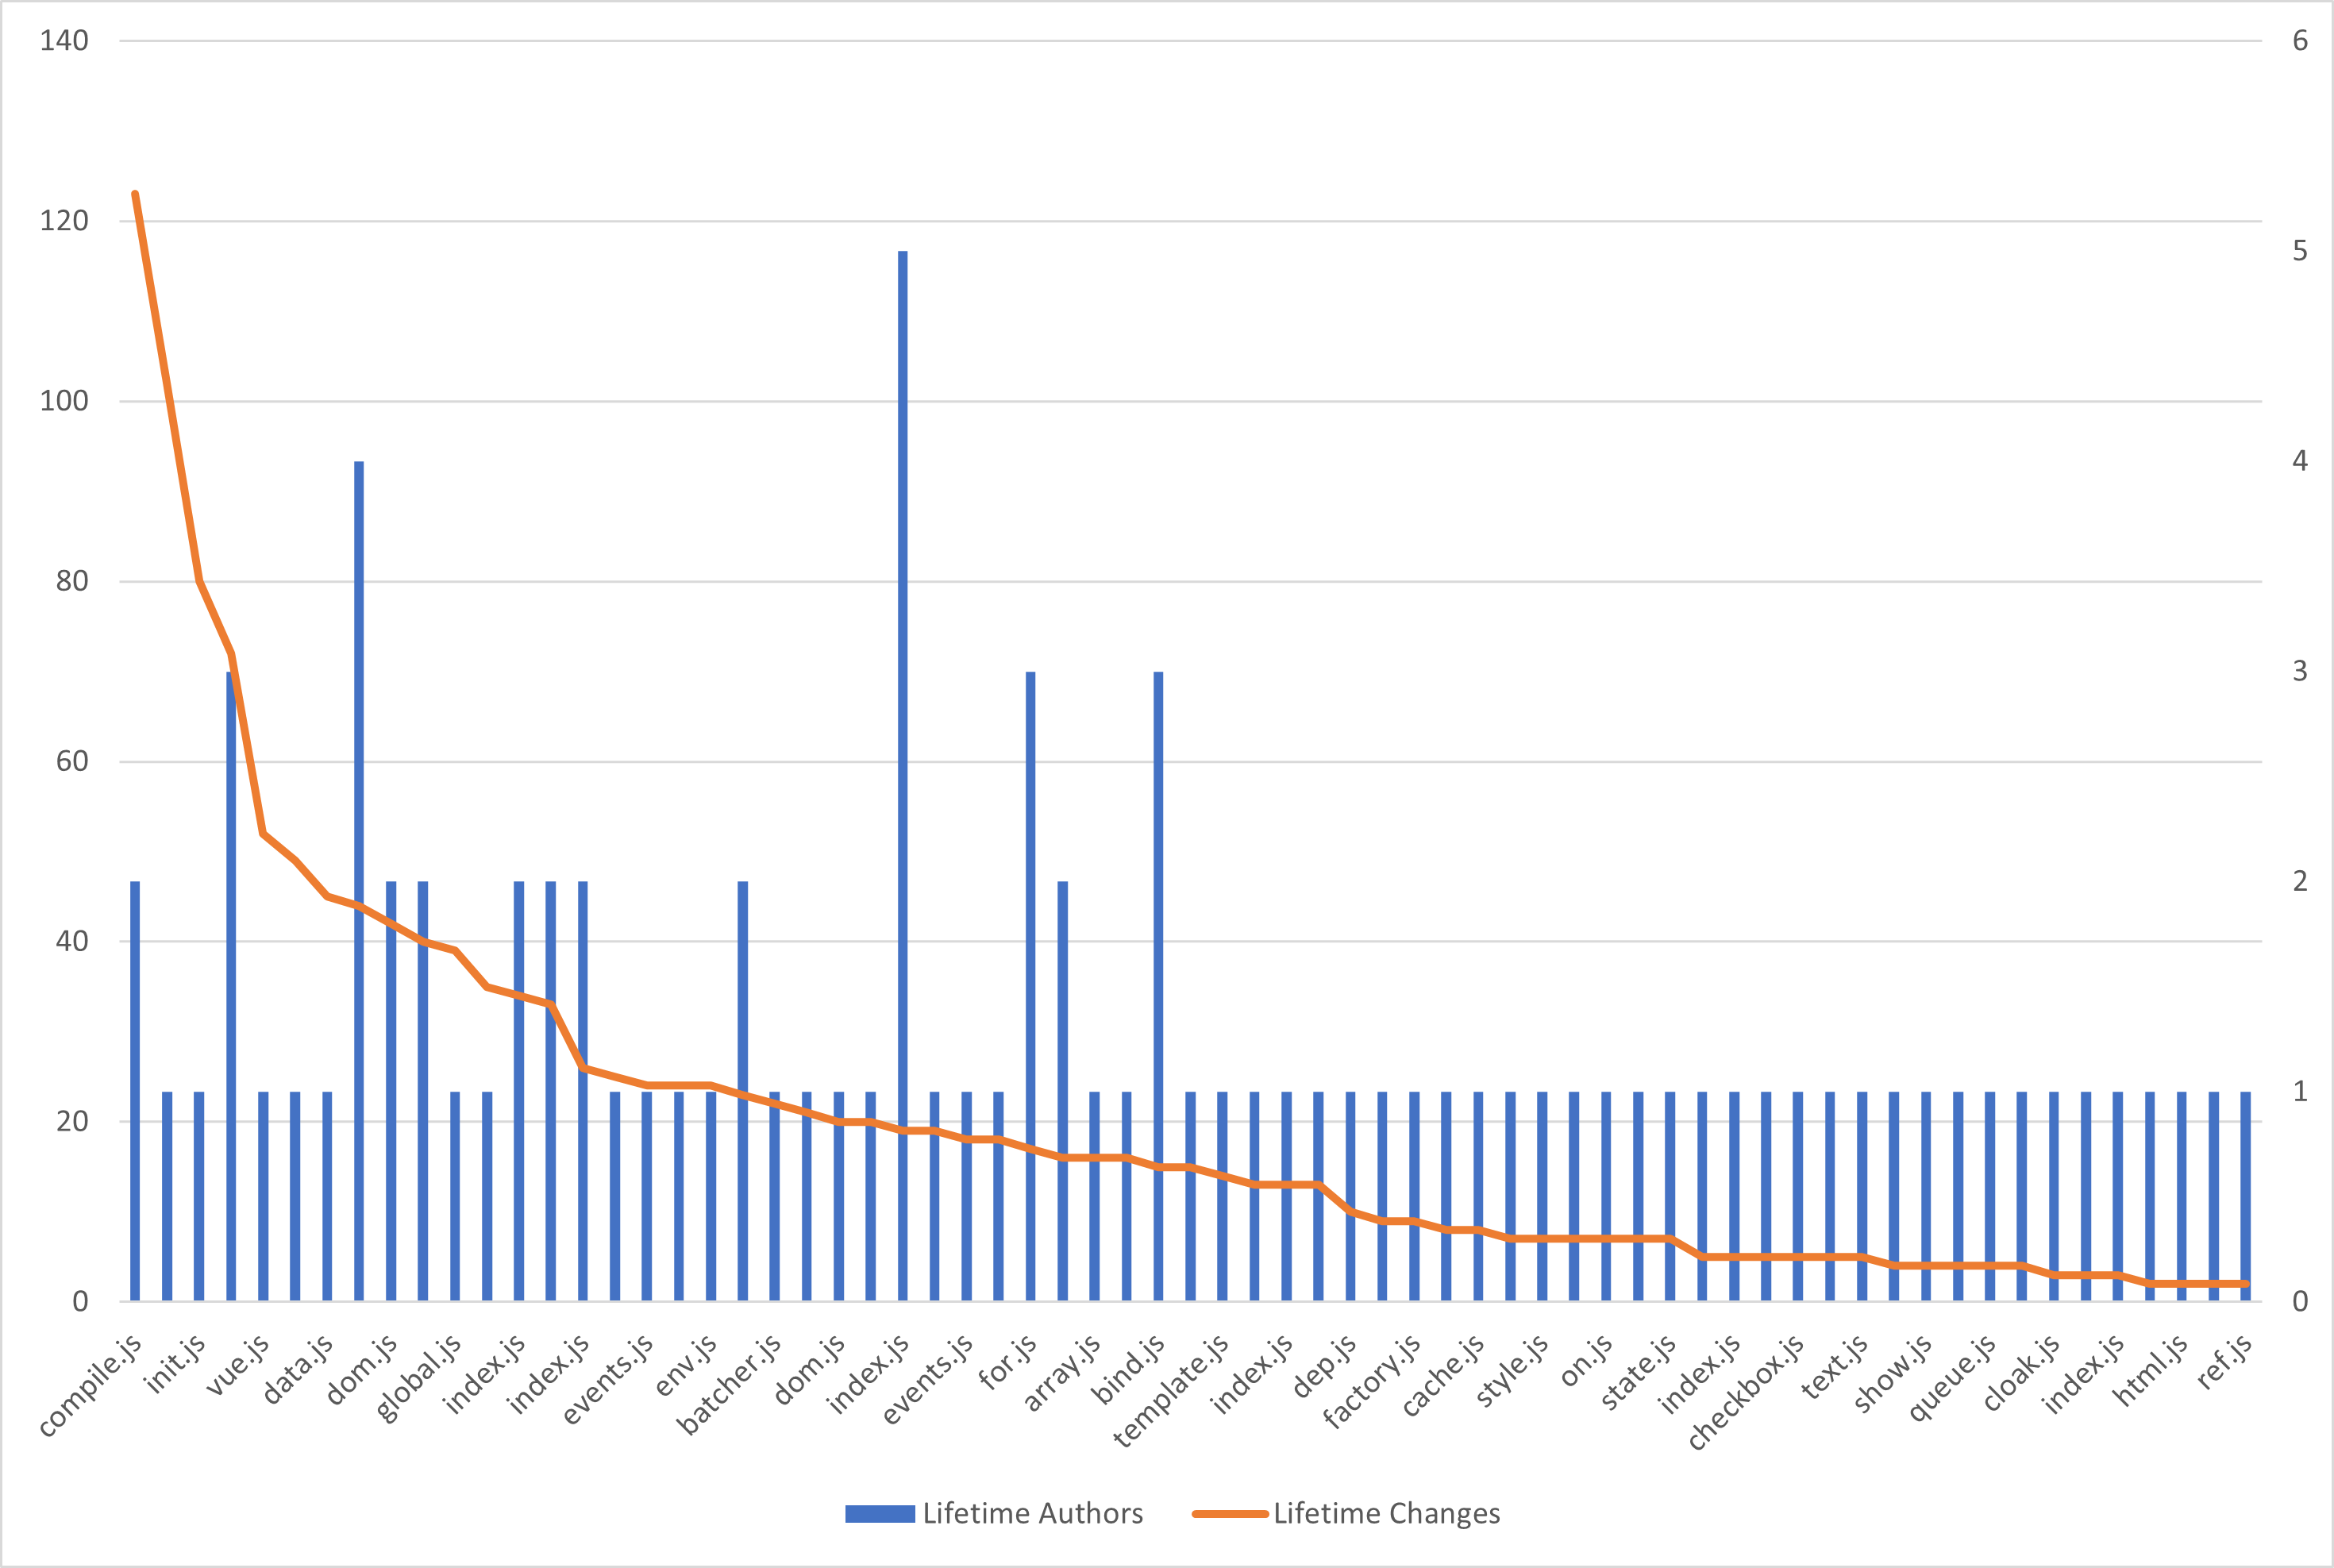
\includegraphics[width=1\textwidth]{images/vue/vue1-lifetimechanges-authors.png}
    \caption{Fájlok módosítási számai és egyedi szerzőinek száma a vue 1.0 esetében}
    \label{fig:vue1-changes-authors}
\end{figure}

Végezetül a \ref{fig:vue1-changes-authors} ábra a fájlok változtatási számát és az egyedi szerzők számát mutatja. A vue ebből a szempontból különleges eset, mert ahogy a \ref{code:vue-authors} kimenetén láttuk a projekt jelentős részben egy fejlesztő kezében van és ez kiemelten igaz az 1.0-ra. A két adatsor között a vue 1.0 esetében a korreláció 0,27.

\begin{figure}[H]
    \centering
    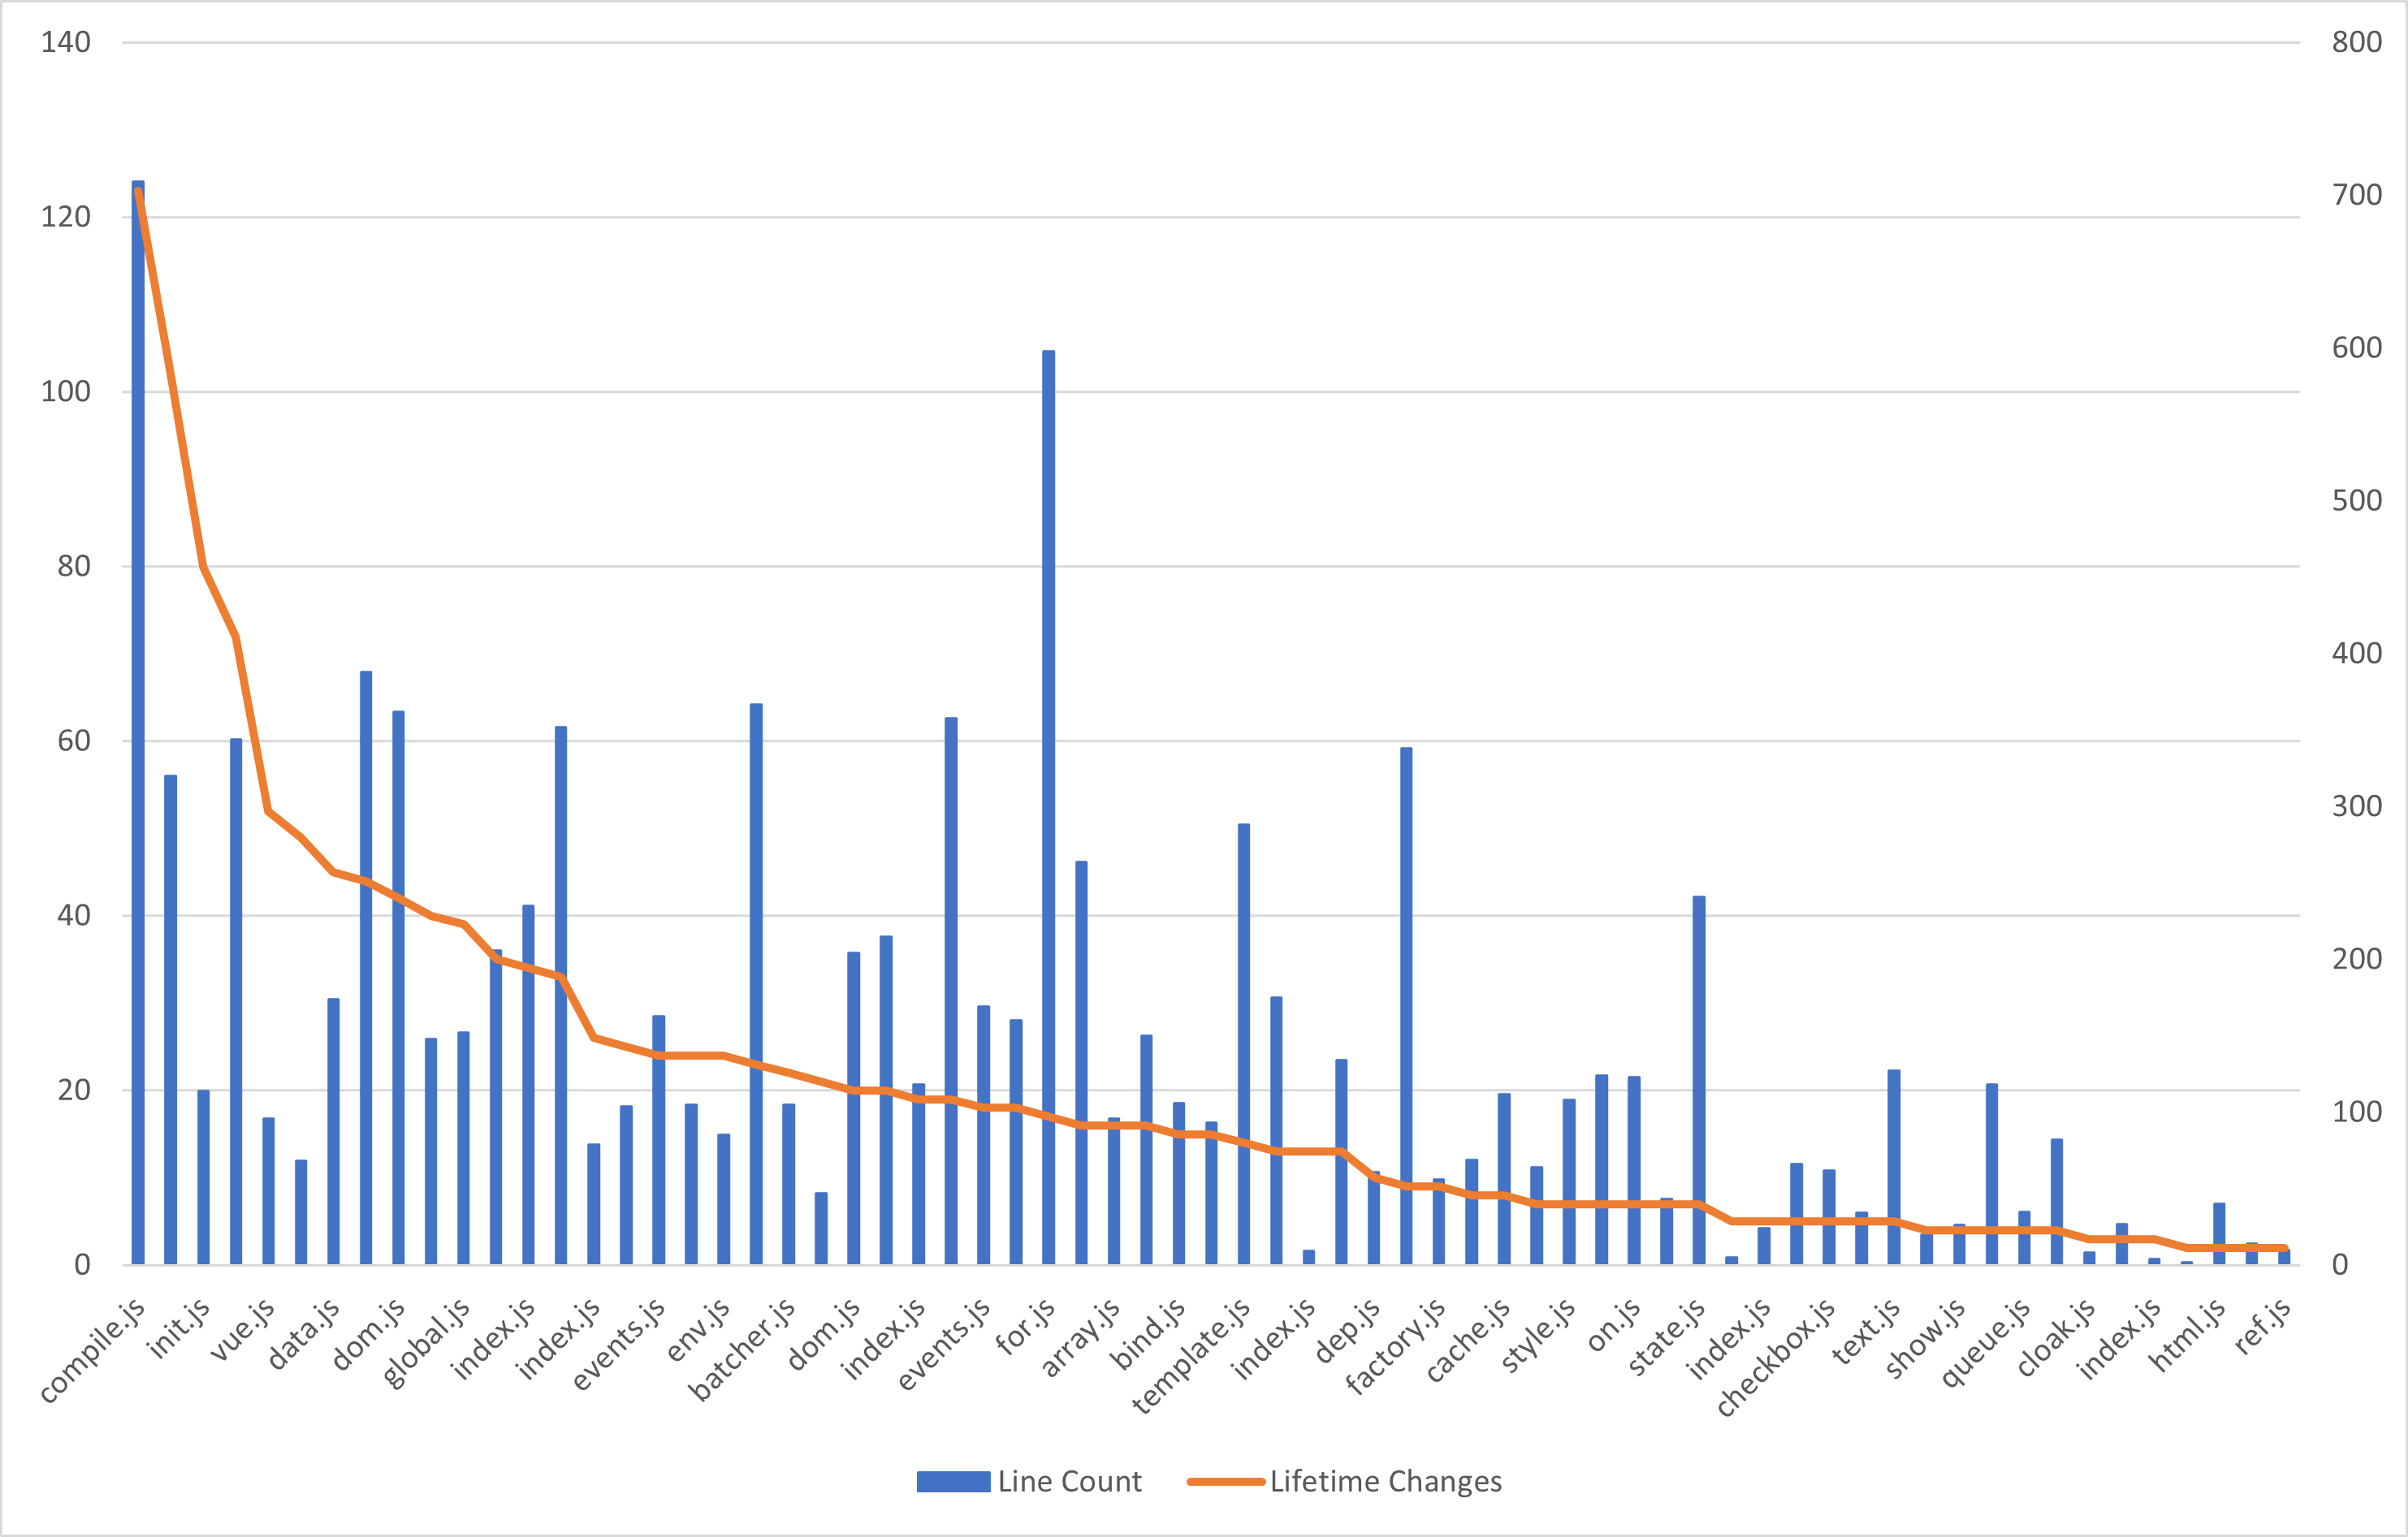
\includegraphics[width=1\textwidth]{images/vue/vue1-lines-lifetimechanges.png}
    \caption{Fájlok módosítási számai és méretük a vue 1.0 esetében}
    \label{fig:vue1-changes-lines}
\end{figure}

\pagebreak

\subsection{Vue 2.0}

A vue 2.0 alig több, mint egy évvel a vue 1.0 után jelent meg, azonban teljes újraírása volt a projektnek, így az 1.0-ban látott adatokkal csak néhány esetben fogunk tudni párhuzamot vonni. A \ref{table:vue2-top-files} táblázat mutatja, hogy a vue 2.0 esetében melyek a legtöbbet változtatott fájlok.

Külön felhívnám a figyelmet a \code{compiler/parser/index.js} és \code{compiler/codegen/index.js} fájlokra és nem csak azért, mert ez a két legtöbbet változtatott fájl. Ezek a fájlok ismerősek lehetnek a vue 1.0-nál látott \code{compile.js} miatt, ami mint az látható a \ref{table:vue1-top-files} táblázatból az akkori állapot legtöbbet változtatott fájlja. Ugyan a git szempontjából nincs kapcsolat a \code{compile.js}, \code{compiler/parser/index.js} és \code{compiler/codegen/index.js} fájlok között, ránézésre azonban hamar kiderül, hogy a \code{compile.js} tovább él a 2.0-ban, két külön fájlra bontva. Ez már most egy érdekes trendet mutat: hiába lett refactor-olva a \code{compile.js}, a szétbontott fájlok pontosan ugyanazt a mintát mutatják, mint az elődjük.

\begin{table}[h]
    \hspace*{-1cm}\begin{tabular}{l|l|l|l|l}
        Filename                     & Lifetime Authors & Lifetime Changes & Line Count & Coverage \% \\ \hline
        compiler/parser/index.js     & 5                & 93               & 467        & 100         \\
        compiler/codegen/index.js    & 2                & 72               & 246        & 100         \\
        render.js                    & 2                & 67               & 253        & 100         \\
        create-component.js          & 4                & 56               & 296        & 100         \\
        patch.js                     & 2                & 54               & 524        & 100         \\
        transition.js                & 1                & 47               & 270        & 100         \\
        lifecycle.js                 & 3                & 45               & 201        & 100         \\
        helpers.js                   & 2                & 34               & 145        & 100         \\
        web-runtime-with-compiler.js & 3                & 33               & 84         & 100         \\
        core/index.js                & 1                & 31               & 13         & 100
    \end{tabular}
    \caption{A vue 2.0-ás kiadásának leggyakrabban módosított fájljai} \label{table:vue2-top-files}
\end{table}

A \code{compile.js} utódait leszámítva azonban a vue 2.0 kódbázisa a \ref{fig:vue2-lifetime-changes} ábra alapján kevésbé polarizált fájl módosítási számok tekintetében, mint a 1.0-ás kiadásban volt. Azt nehéz viszont megítélni, hogy ez fedi-e a valóságot, vagy csak a git technikalitása a teljes újraírás miatt, hiszen láttuk, hogy a \code{compile.js} két utódja teljesen tiszta lappal indult és ugyanez a minta előfordulhat kevésbé egyértelmű szituációkban is.

\begin{figure}[H]
    \centering
    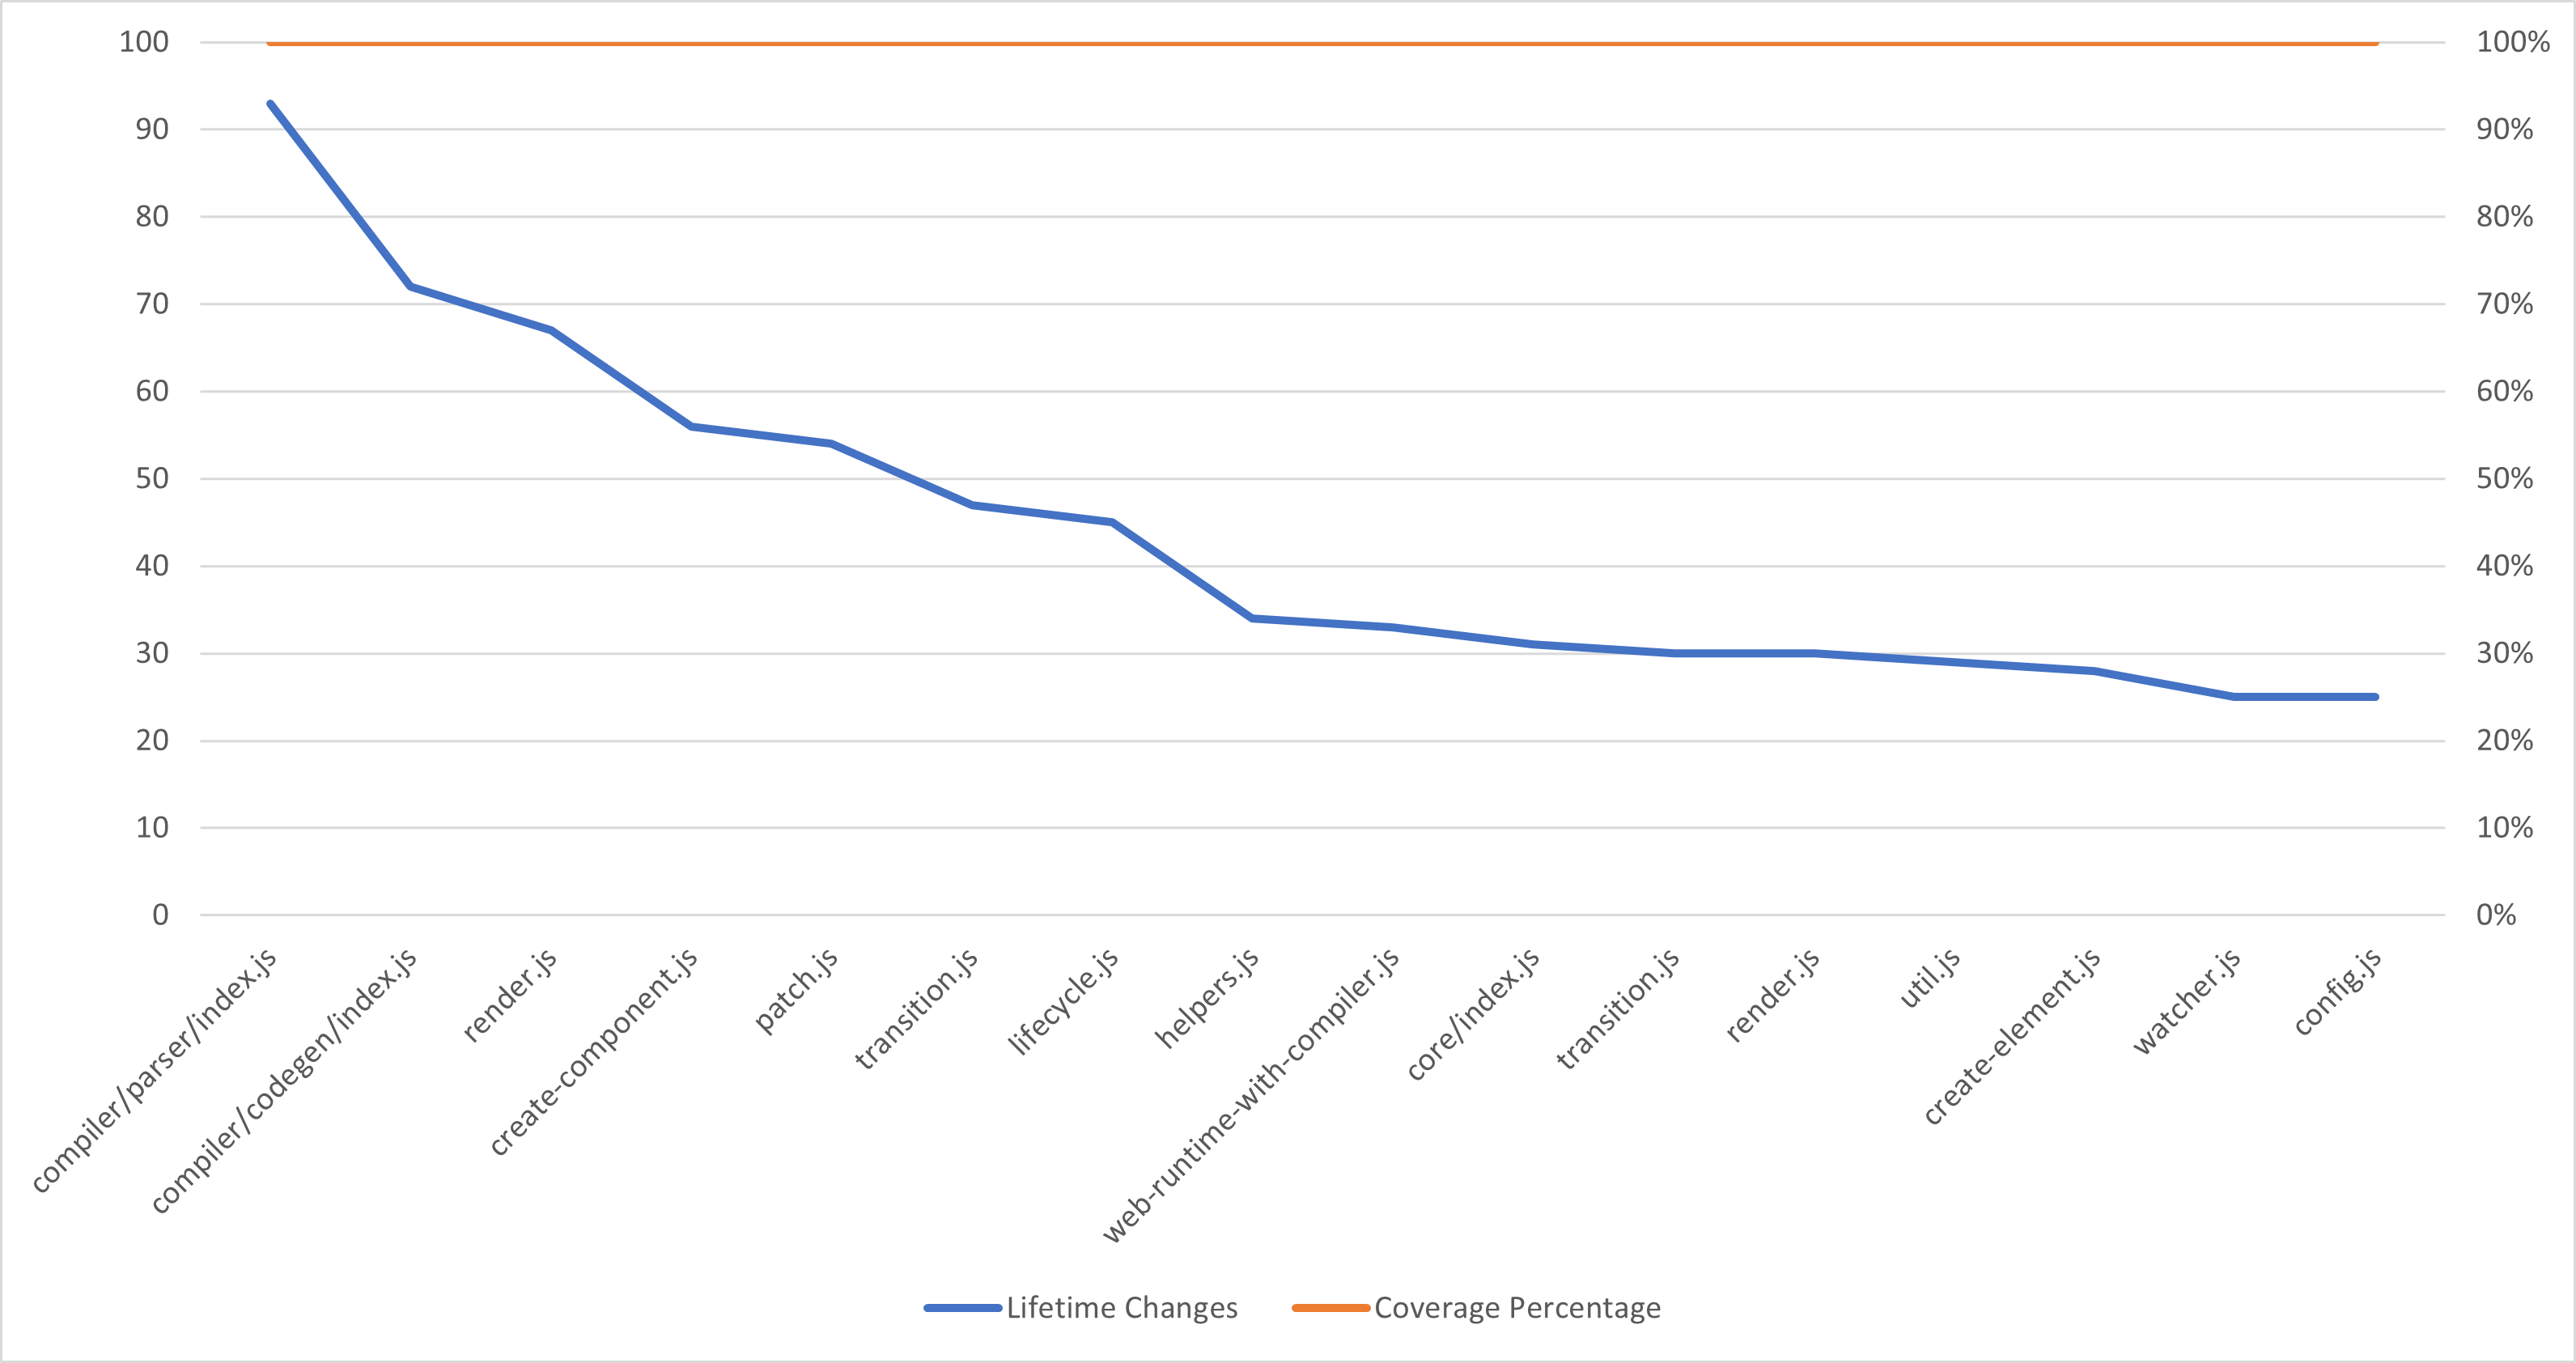
\includegraphics[width=1\textwidth]{images/vue/vue2-lifetime-changes.png}
    \caption{Fájlok módosítási számai a vue 2.0.1 esetében}
    \label{fig:vue2-lifetime-changes}
\end{figure}

A módosítási számok hisztogramja a \ref{fig:vue2-hist} nagyon hasonló képet fest a korábbiakban látottakhoz. A 2.0 kódbázisának túlnyomó többsége ismét a ritkán módosított fájlokba tömörül, azonban a leggyakrabban módosított felső 10\% újfent az átlagos módosítási szám sokszorosát produkálja.

\begin{figure}[H]
    \centering
    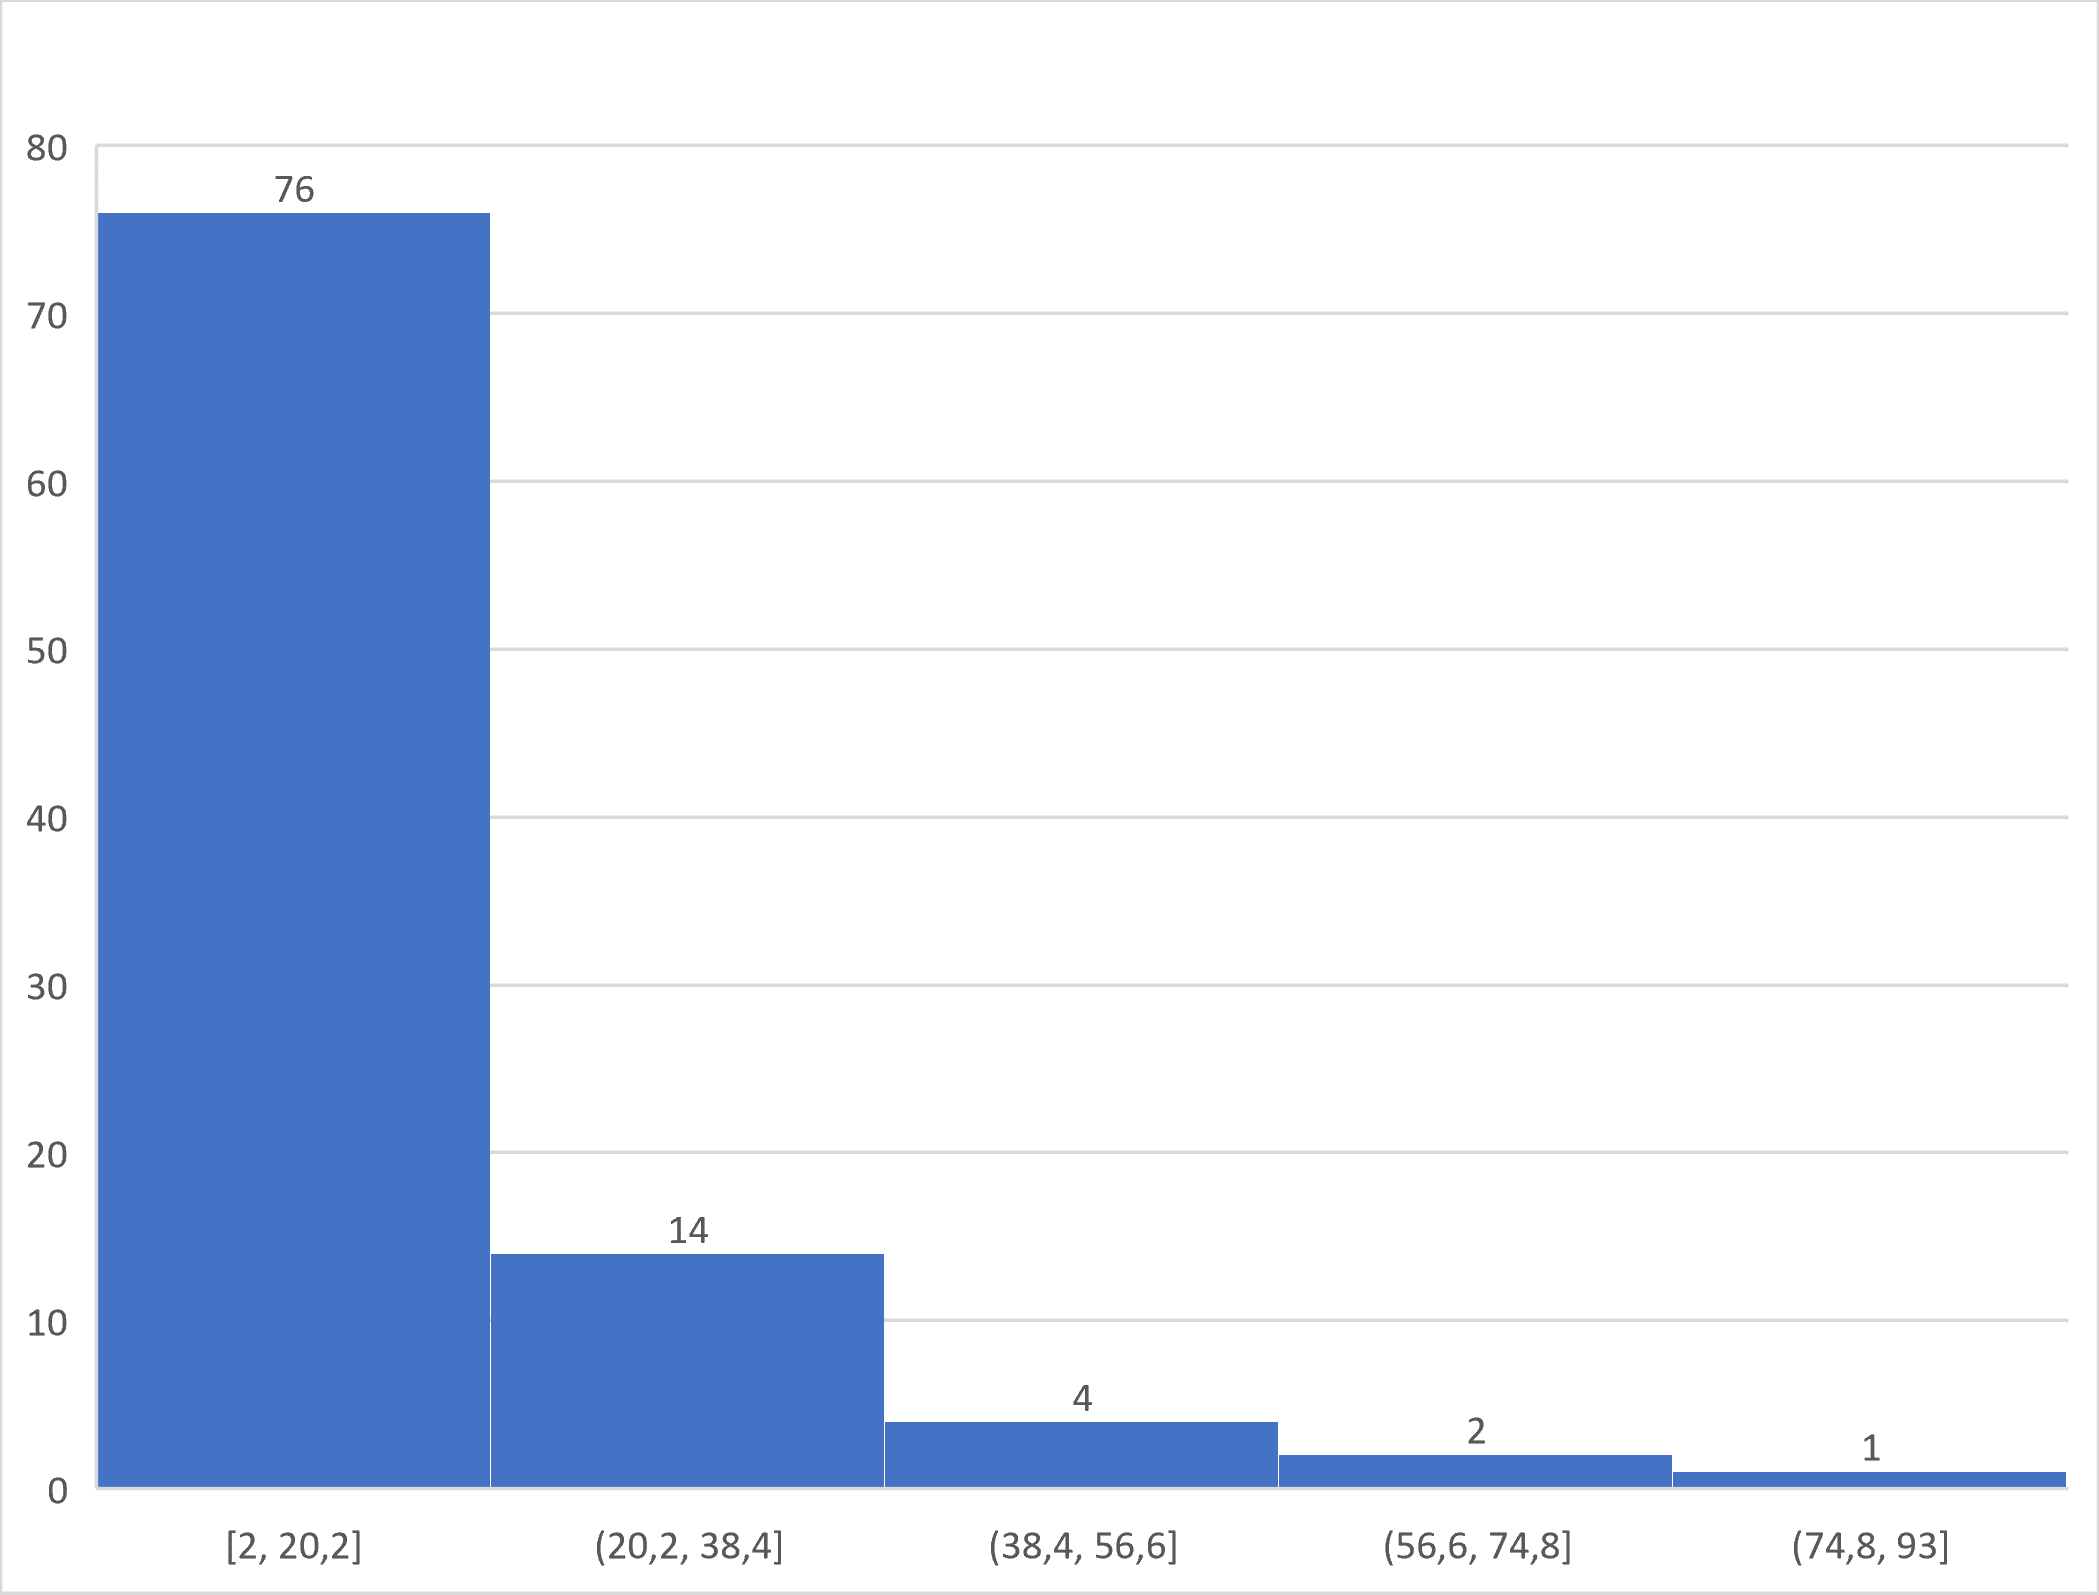
\includegraphics[width=1\textwidth]{images/vue/vue2-hist.png}
    \caption{Fájlok módosítási számának hisztogramja a vue 2.0.1 esetében}
    \label{fig:vue2-hist}
\end{figure}

Végül vegyük szemre a \ref{fig:vue2-lines-changes} ábrát, ami a fájlok módosítási számait és méretét mutatja. Ellentétben az 1.0-ban látottakkal, a 2.0 kódbázisa esetében a fájlok méretéből rajzolt görbe sokkal közelebb követi le a módosítási számokból rajzolt görbét.

\begin{figure}[H]
    \centering
    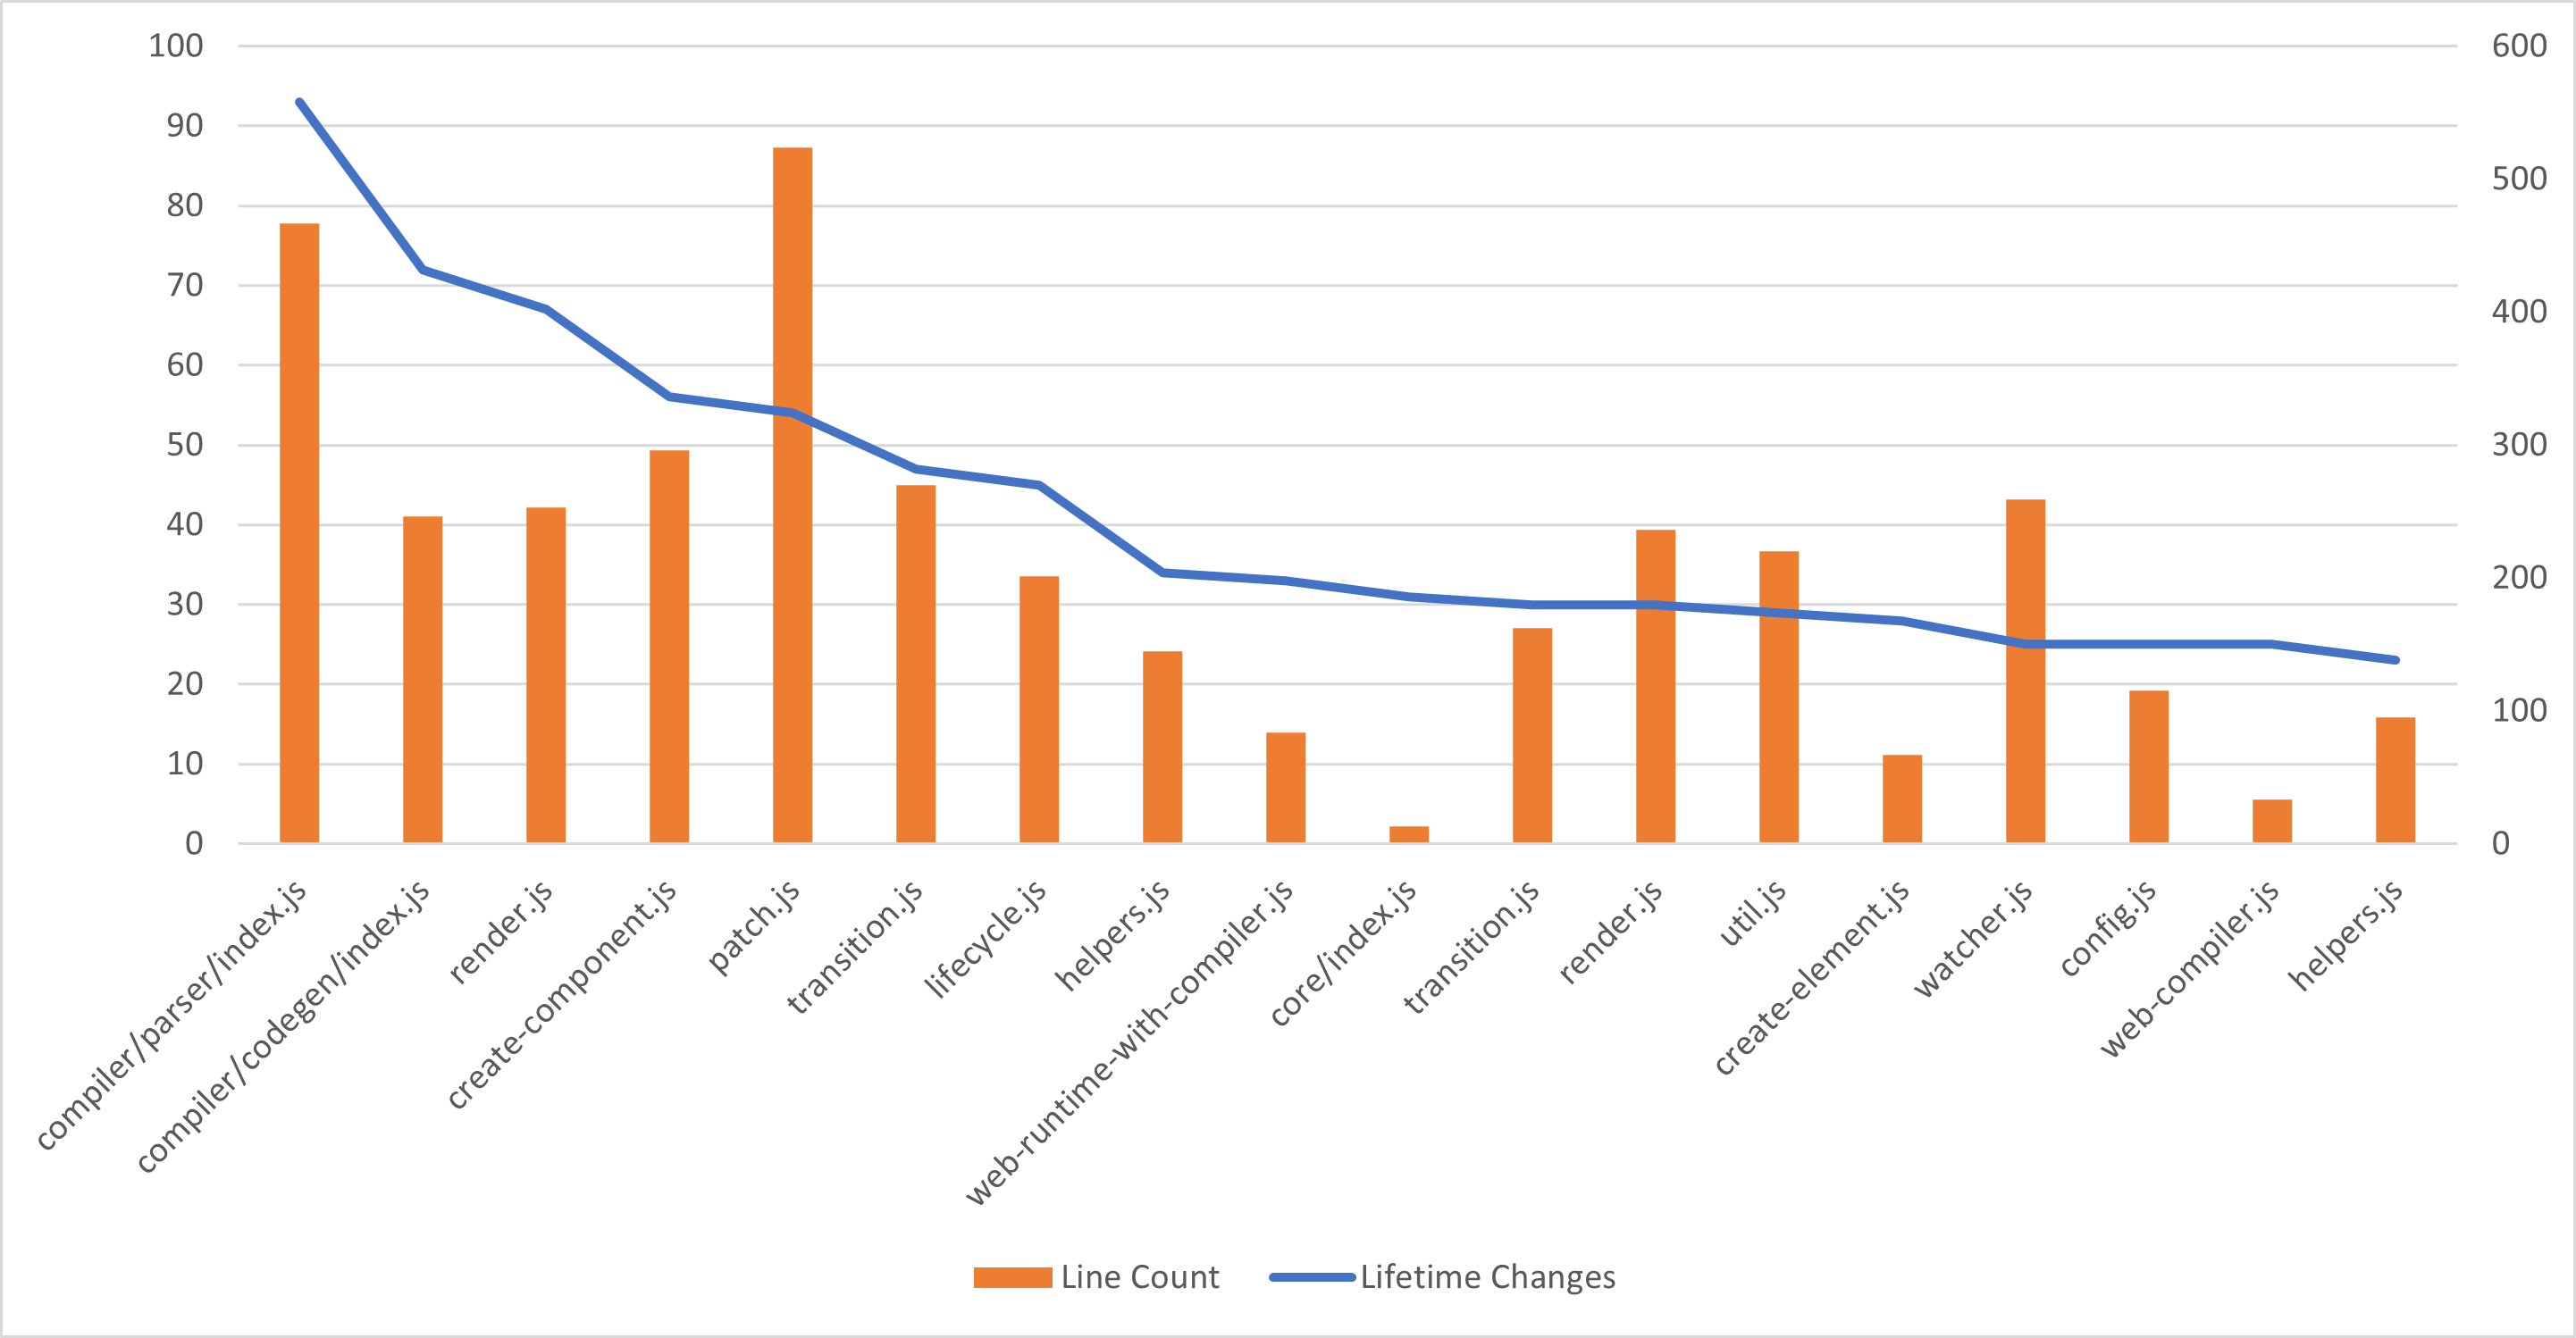
\includegraphics[width=1\textwidth]{images/vue/vue2-lines-lifetimechanges.png}
    \caption{A vékony kliens által generált grafikonok}
    \label{fig:vue2-lines-changes}
\end{figure}

\subsection{Trendek a vue 2.0, 2.4 és a legfrissebb verzió között}

Mielőtt levonnánk néhány tanulságot, nézzük meg, hogy hogyan alakult a vue kódbázisa a 2016-ban megjelent 2.0-ás verzió és a jelenlegi, 2020-as éles verzió között. A \ref{tab:vue-changes-comp} táblázat mutatja a fájlok módosítási számát 2.0.1 és a legfrissebb verzió között, a 2.0.1-es változtatási szám szerinti csökkenő sorrendben. Ugyan ez a táblázat csak a top 10 fájlt mutatja, de itt is egyértelműen látszódik egy trend, ami egyébként a teljes, 90 fájlból álló kódbázisra is igaz: ha egy fájlt sokat kellett módosítani a projekt életciklusának elején, akkor sokat kellett módosítani később is, amíg a keveset változtatott fájlok jellemzően kevés változtatásra szorulnak a teljes életciklusuk alatt. Nem meglepő módon így a korreláció a 2.0.1-es és a legfrissebb verzió változtatási számai között nagyon magas, 0,965.

\begin{table}[h]
    \centering
    \begin{tabular}{l|l|l|l|l}
        Filename                  & 2.0.1 & 2.4.0 & master & delta \\ \hline
        compiler/parser/index.js  & 93    & 149   & 206    & 113   \\
        compiler/codegen/index.js & 72    & 121   & 160    & 88    \\
        render.js                 & 67    & 105   & 122    & 55    \\
        create-component.js       & 56    & 91    & 112    & 56    \\
        patch.js                  & 54    & 92    & 119    & 65    \\
        transition.js             & 47    & 68    & 73     & 26    \\
        lifecycle.js              & 45    & 76    & 96     & 51    \\
        core/index.js             & 31    & 47    & 48     & 17    \\
        render.js                 & 30    & 60    & 72     & 42    \\
        transition.js             & 30    & 49    & 54     & 24
    \end{tabular}
    \caption{A vue.js legtöbbet változtatott fájljai 2.0 és az aktuális verzió között}
    \label{tab:vue-changes-comp}
\end{table}

A \ref{fig:vue-all-files-lifetime-changes} ábra új rendezési szempont szerint mutatja be a projekt összes fájlját módosítások száma szerint, a legújabb verzióban megfigyelt érték szerint csökkenő sorrendben. Ezen az ábrán két nagyon szembetűnő tény figyelhető meg:
\begin{itemize}
    \item A fájlok módosítási számai közötti erőviszonyok négy évnyi változtatás során sem változtak, a polarizáltság változatlanul nagyon magas
    \item Új változási gócpontot képező fájlok nem alakultak ki
\end{itemize}

A \ref{fig:vue-all-delta-hist} hisztogram a vue 2.0 és a legfrissebb verzió között megfigyelt fájl módosítások deltáit csoportosítja, azaz azt, hogy a két verzió között hány változtatás érintette az adott fájlokat. Ahogy várható, ez a hisztogram tökéletesen leköveti a 2.0-tól megfigyelt változtatási számokból képzett hisztogramokat, tovább erősítve az eddig megfigyelt trendeket.

\begin{figure}[H]
    \centering
    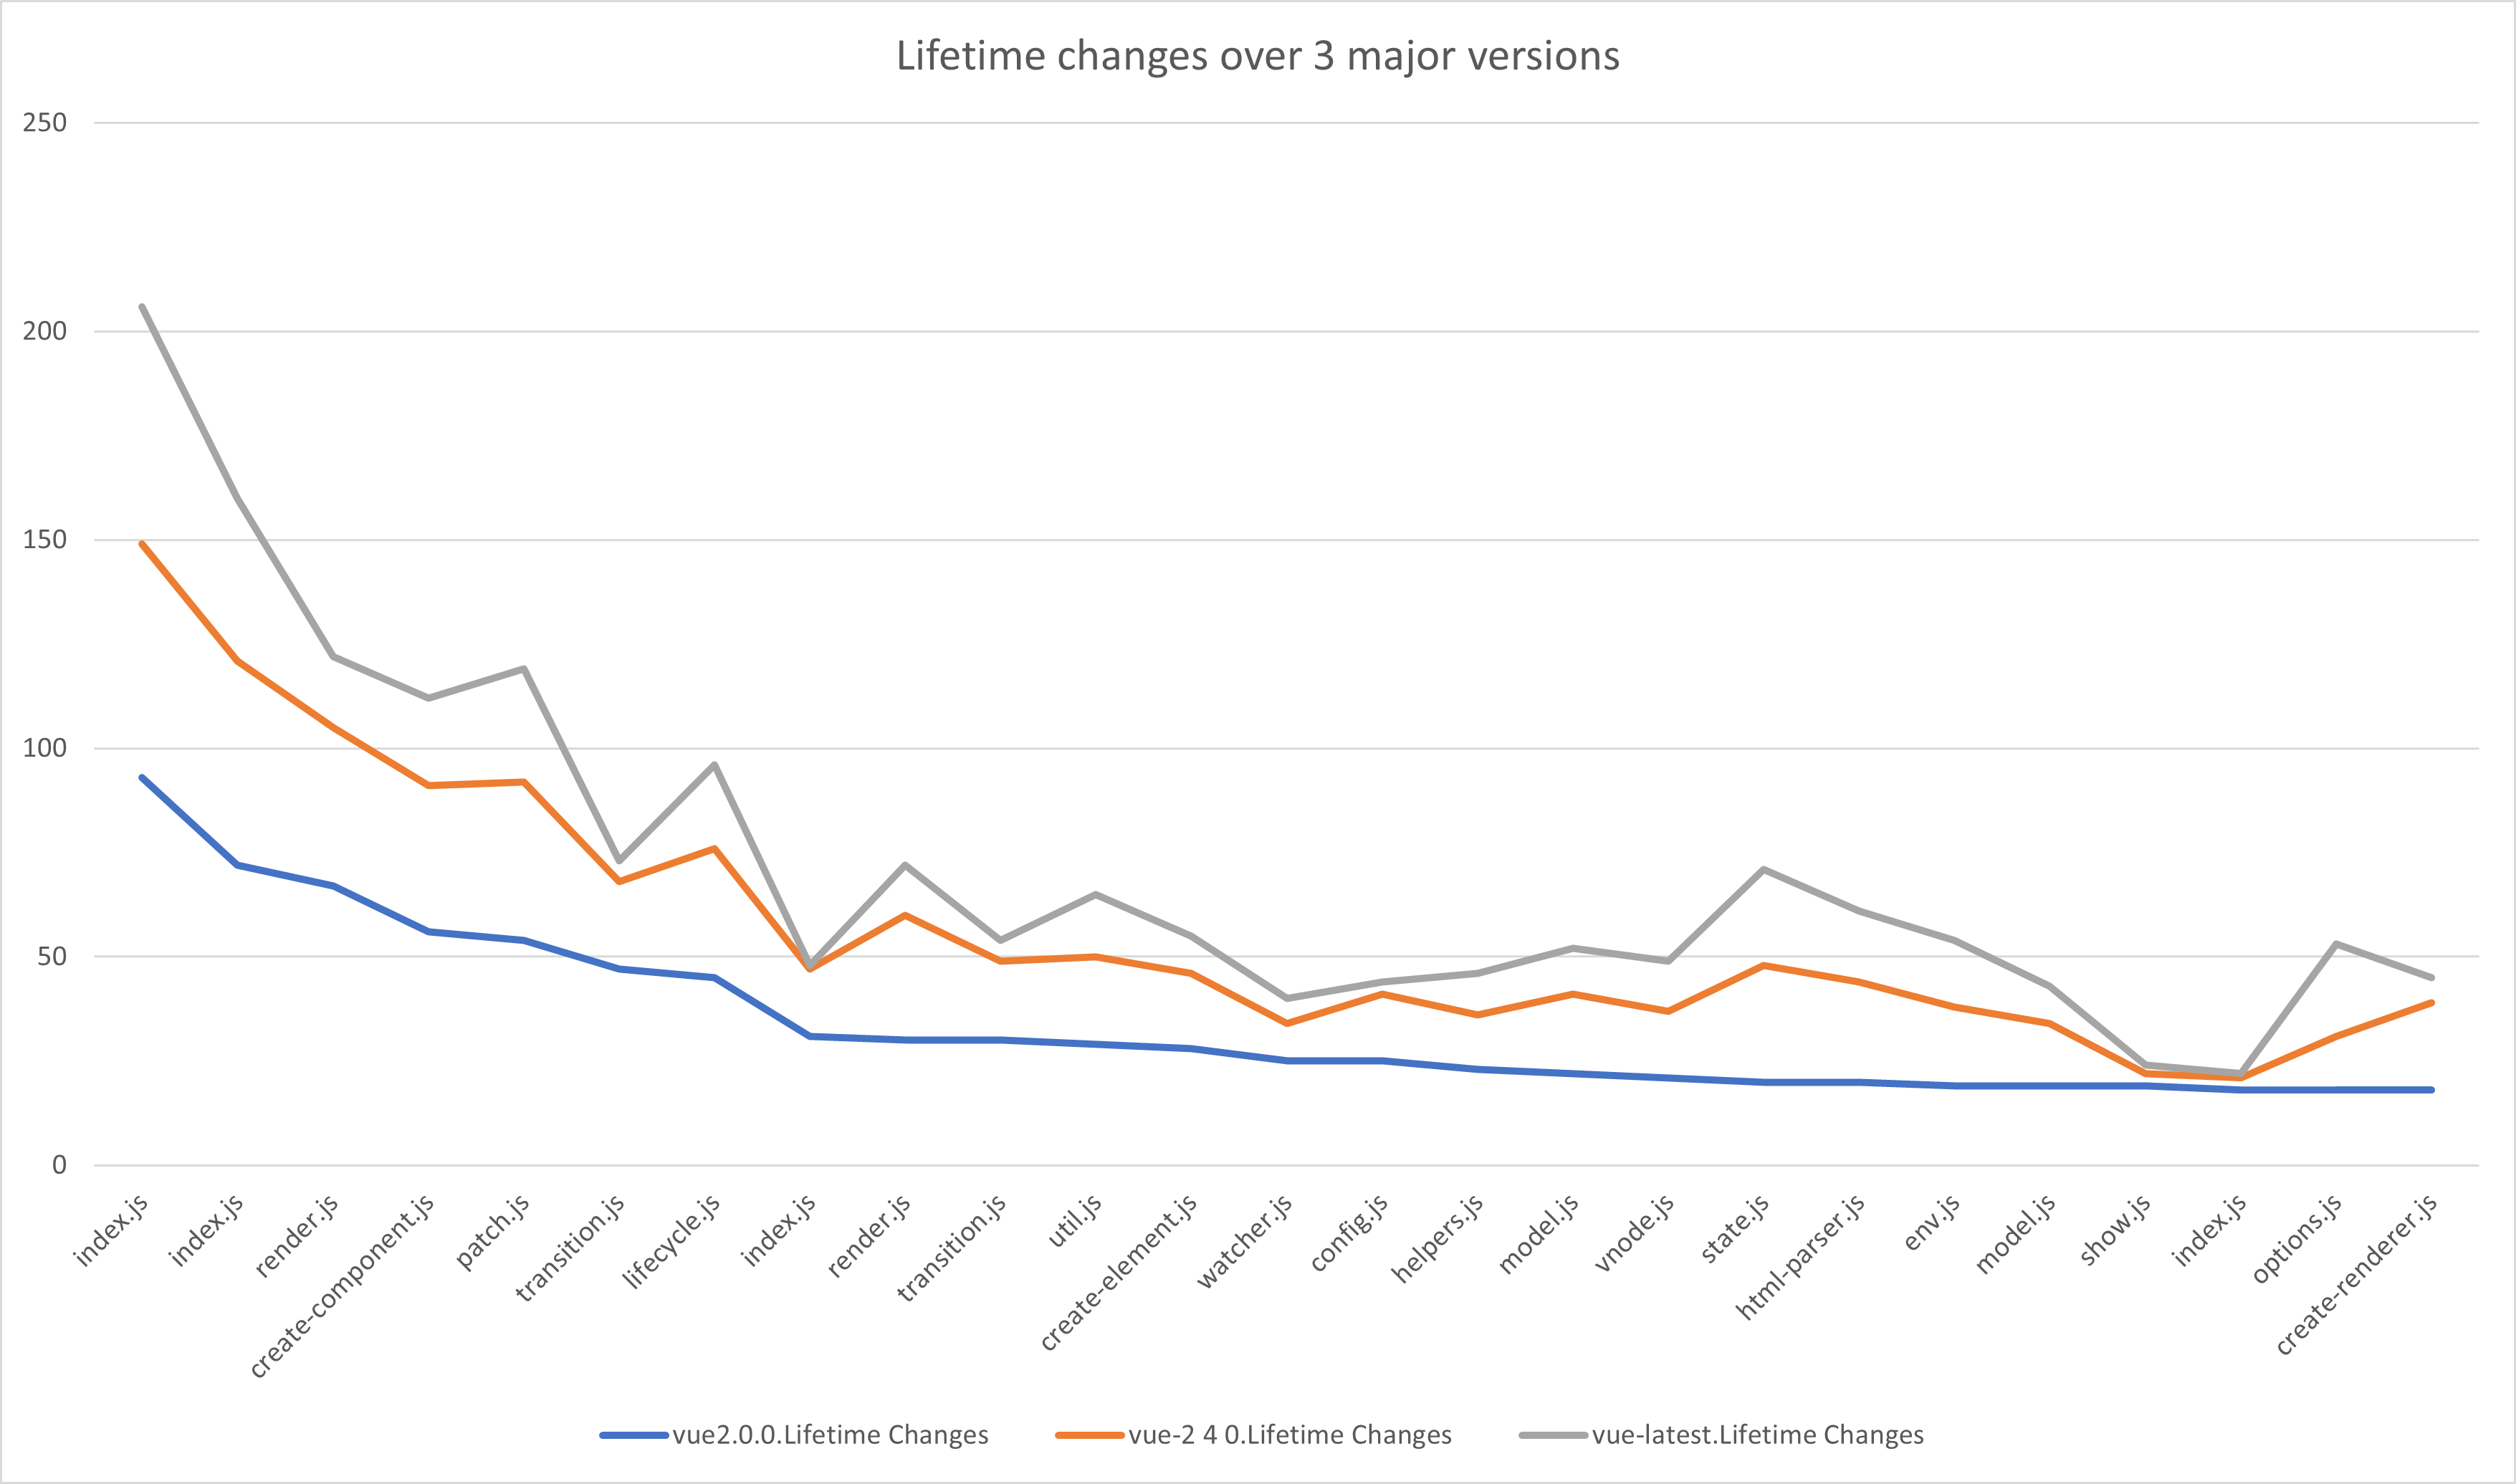
\includegraphics[width=1\textwidth]{images/vue/vue-all-lifetime-changes.png}
    \caption{A vue legtöbbet módosított fájljainak alakulása 2016 és 2020 között}
    \label{fig:vue-all-top-files}
\end{figure}

\begin{figure}[H]
    \centering
    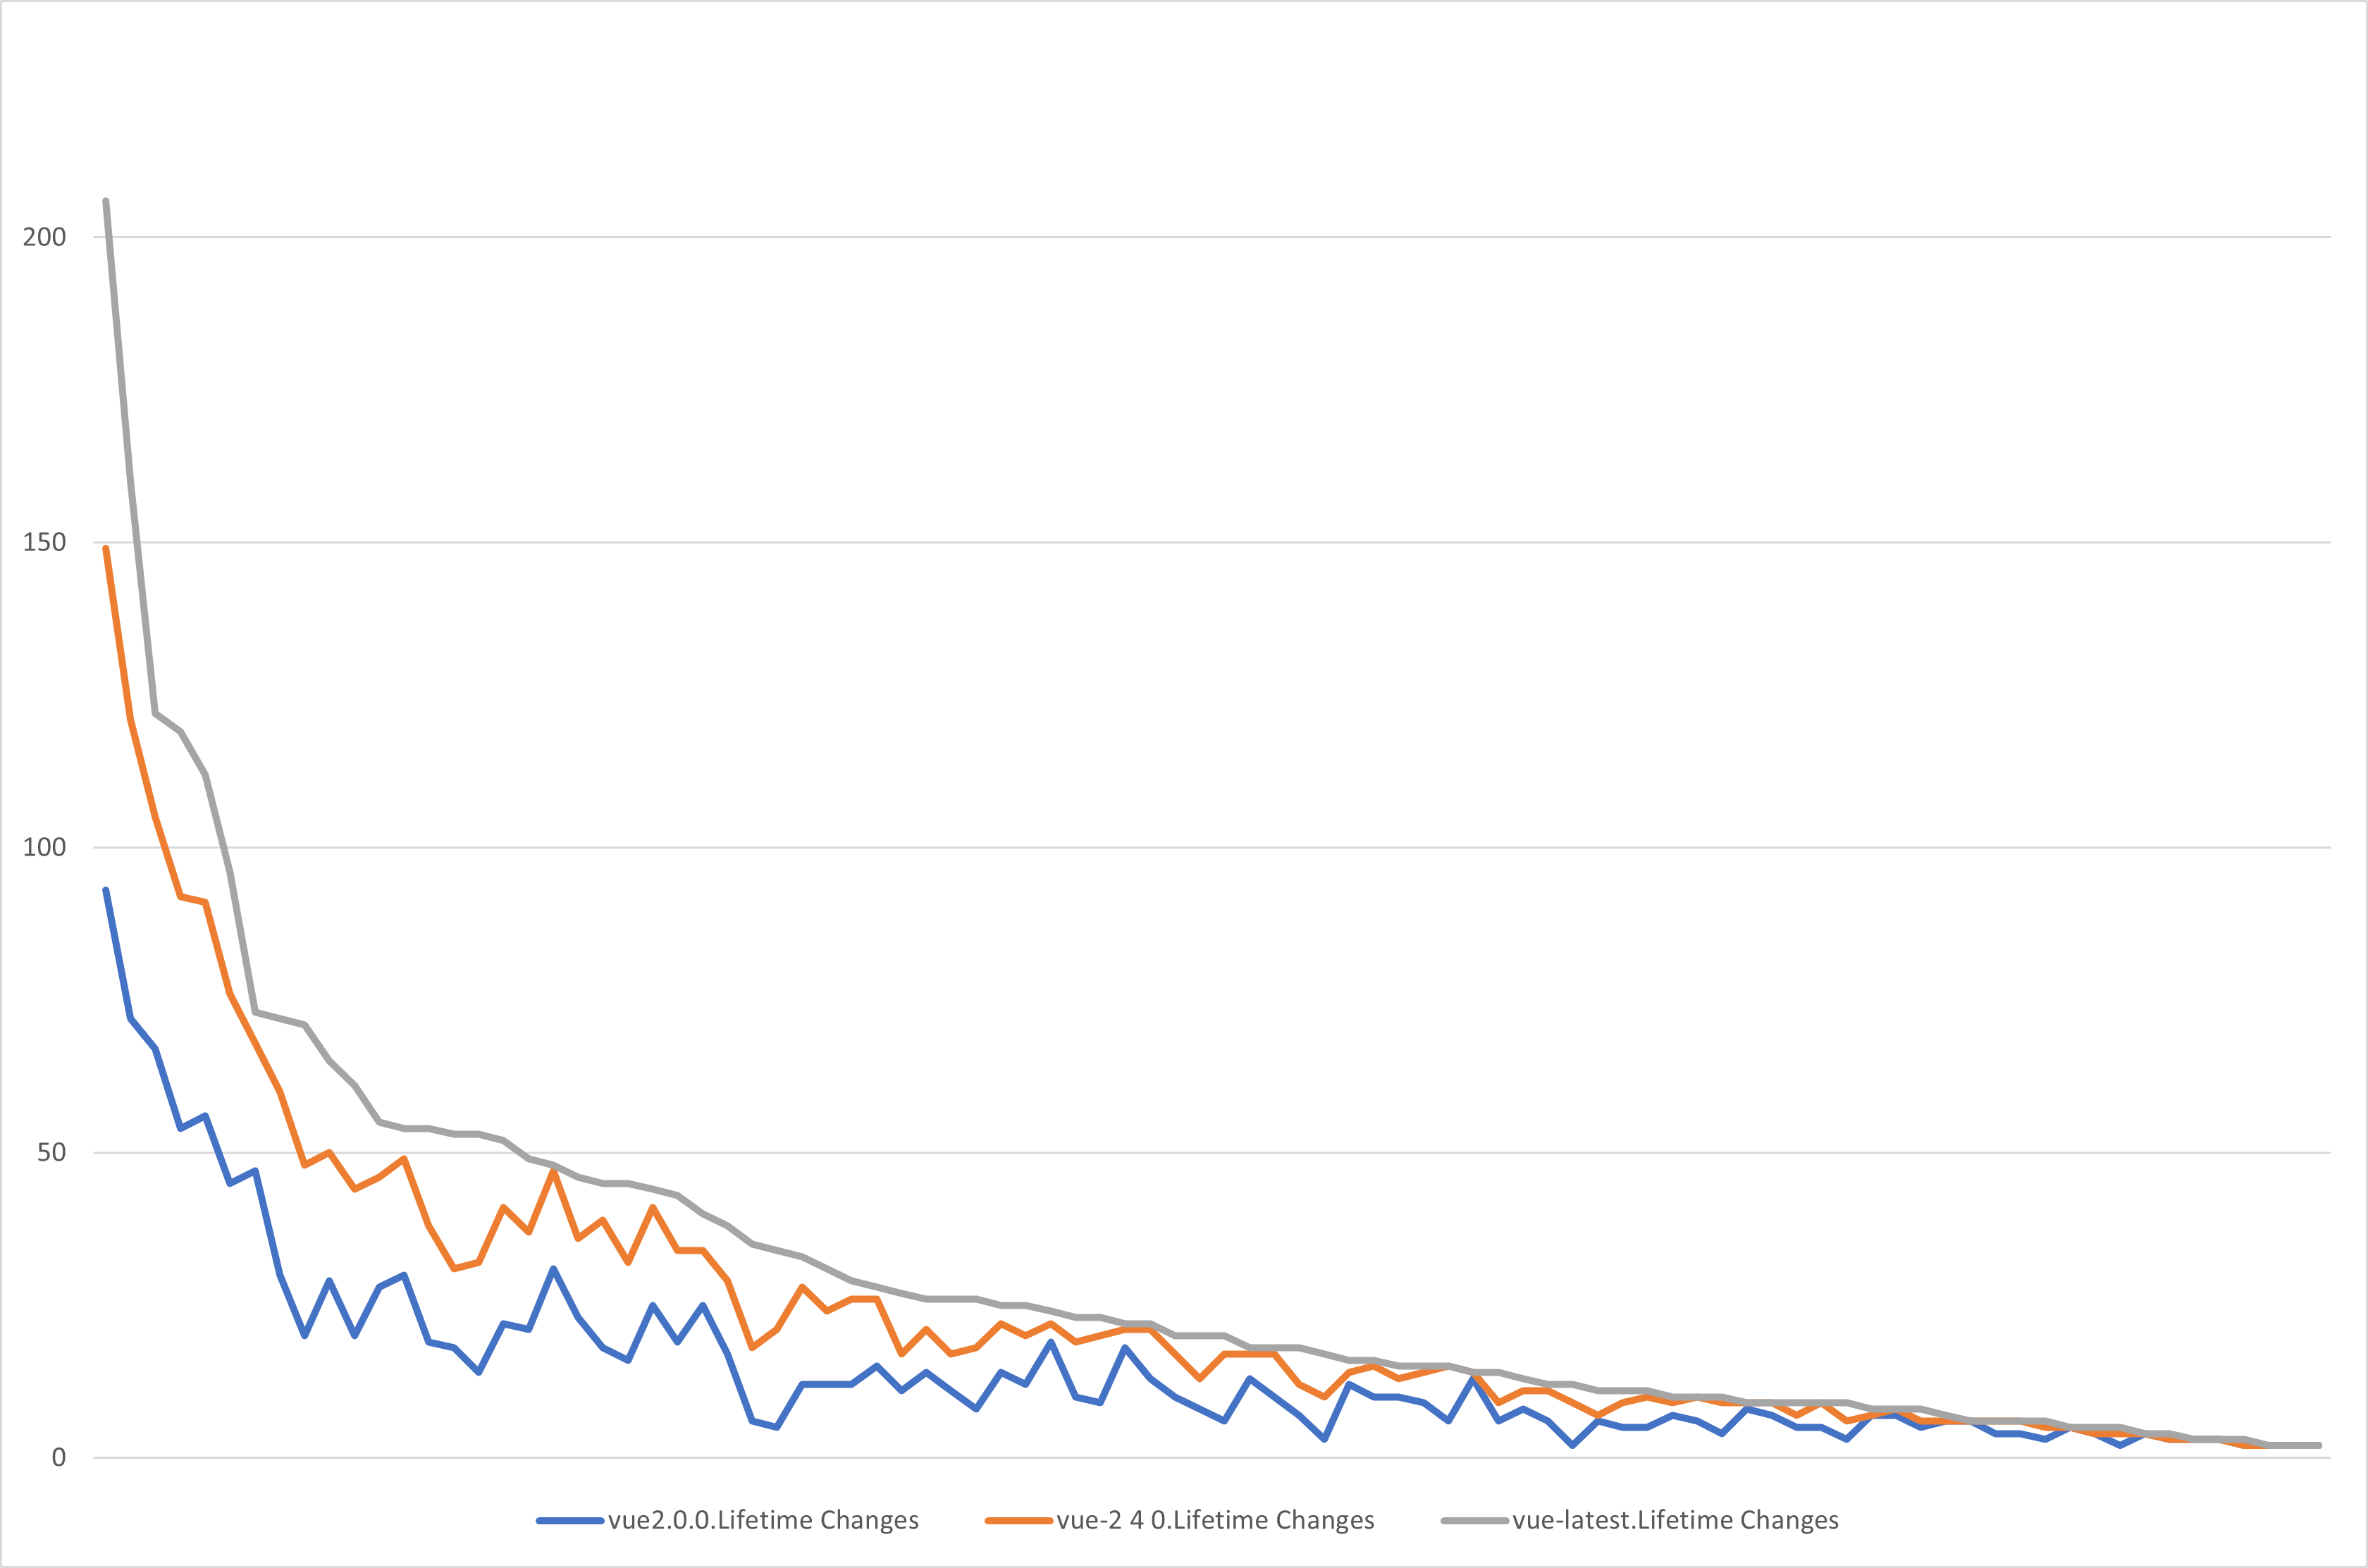
\includegraphics[width=1\textwidth]{images/vue/vue-all-lifetime-changes-comp-full.png}
    \caption{A vue projekt összes fájljának módosítási számai}
    \label{fig:vue-all-files-lifetime-changes}
\end{figure}

\begin{figure}[H]
    \centering
    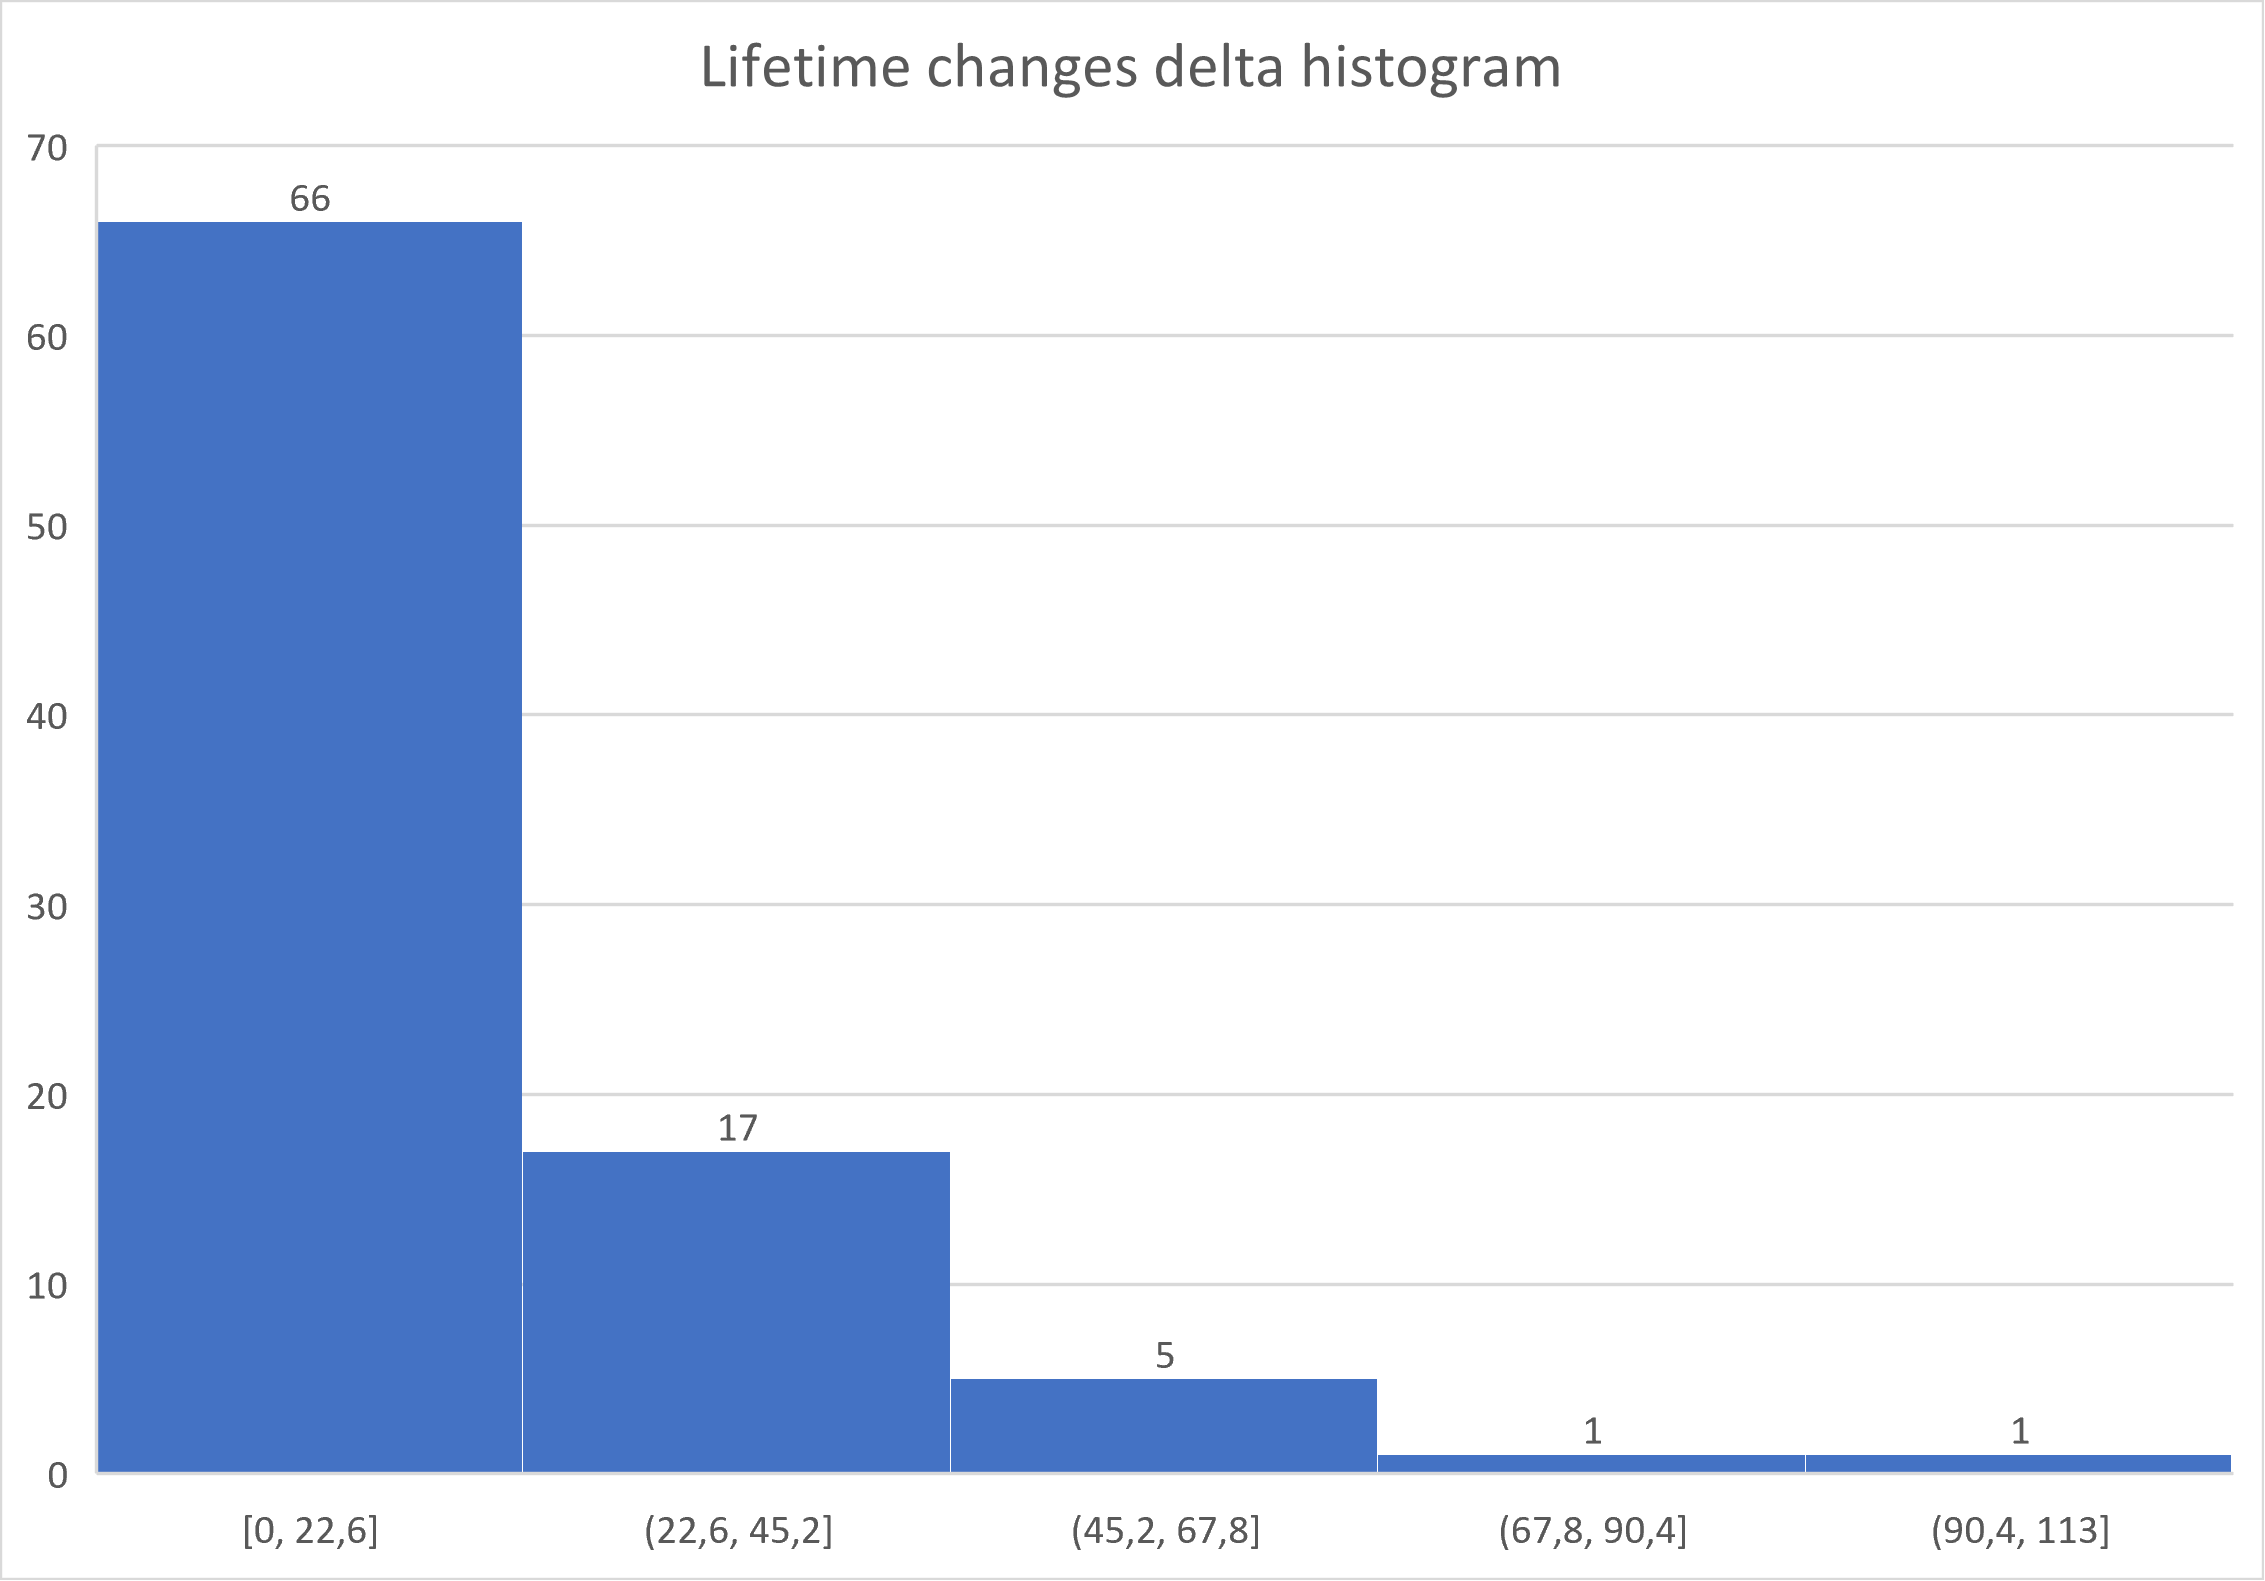
\includegraphics[width=1\textwidth]{images/vue/vue-all-lifetime-changes-delta-hist.png}
    \caption{A vue projekt 2.0-ás és legfrissebb verzióiban lévő fájlok módosítási számainak deltái}
    \label{fig:vue-all-delta-hist}
\end{figure}

\begin{figure}[H]
    \centering
    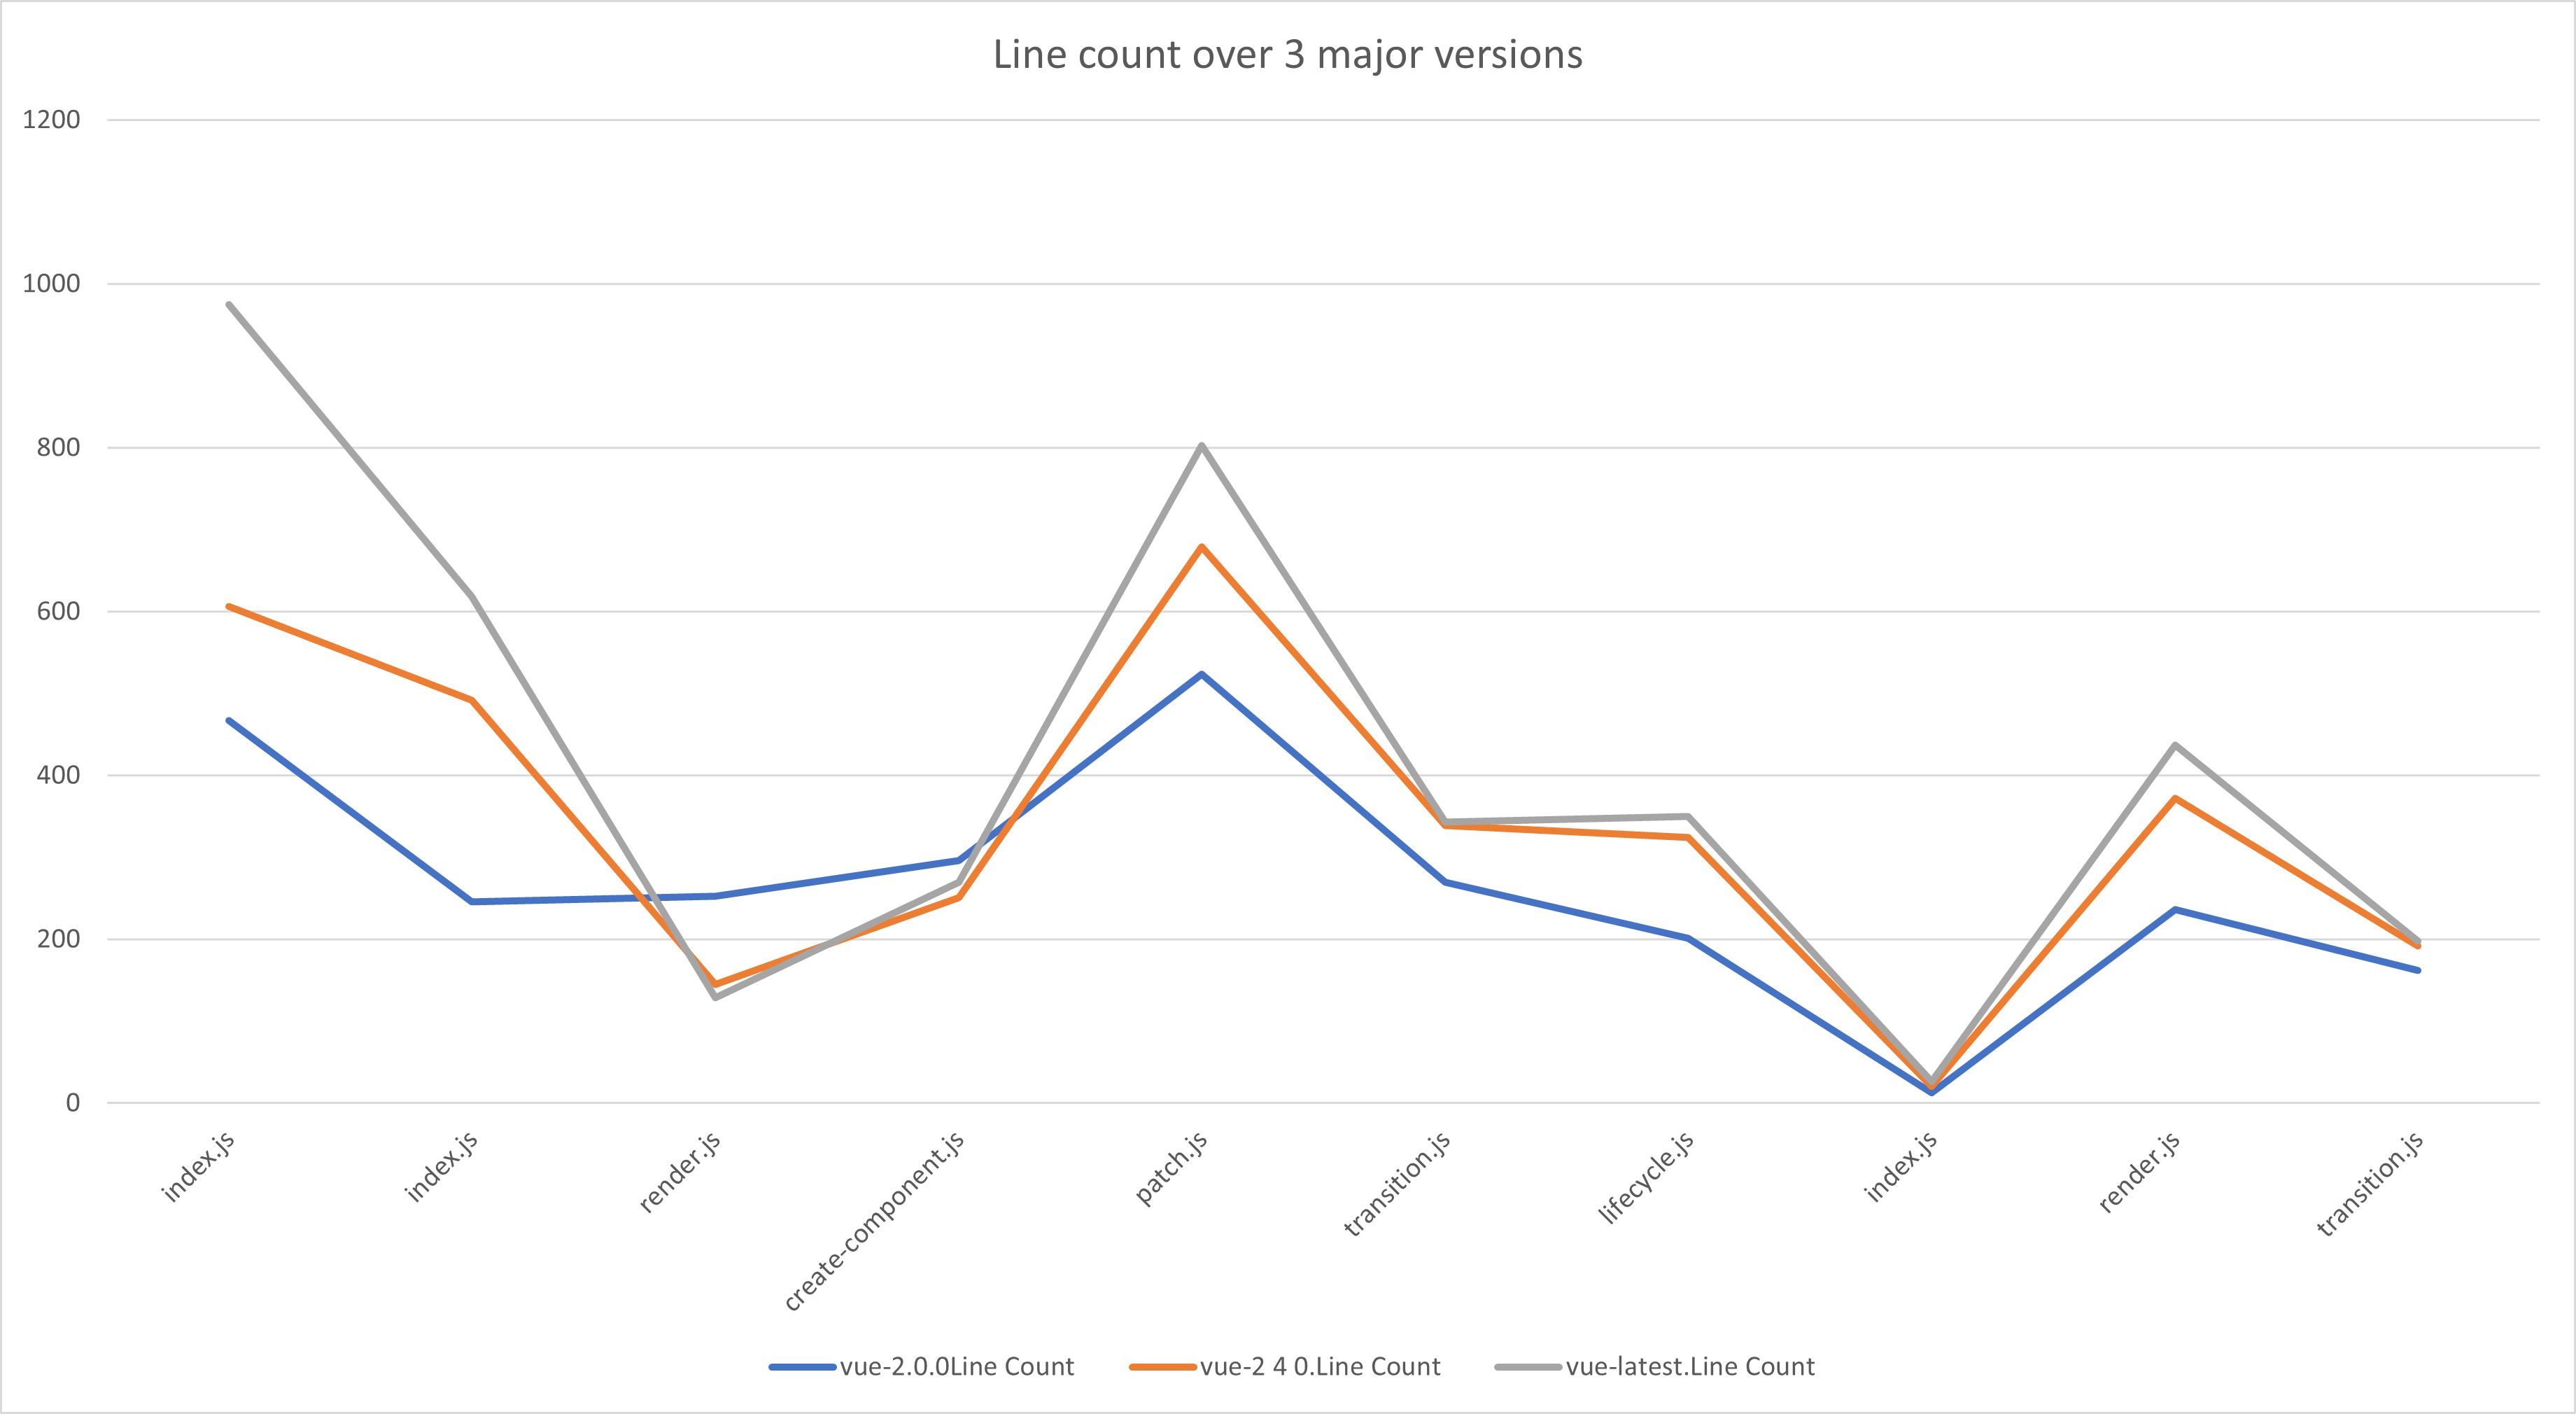
\includegraphics[width=1\textwidth]{images/vue/vue-all-line-count.png}
    \caption{A vue projektben lévő fájlok méretének változása 3 verzión keresztül}
    \label{fig:vue-all-line-count}
\end{figure}

Végül tekintsük a \ref{fig:vue-all-delta-hist} ábrát, amin a fájlok coverage-e látható. Kijelenthetjük, hogy a vue esetében a teszt coverage semmilyen moderáló hatást nem gyakorolt a változtatási gócpontokra, illetve a gócpontok növekedése nem hatott negatívan a unit tesztekre.

\begin{figure}[H]
    \centering
    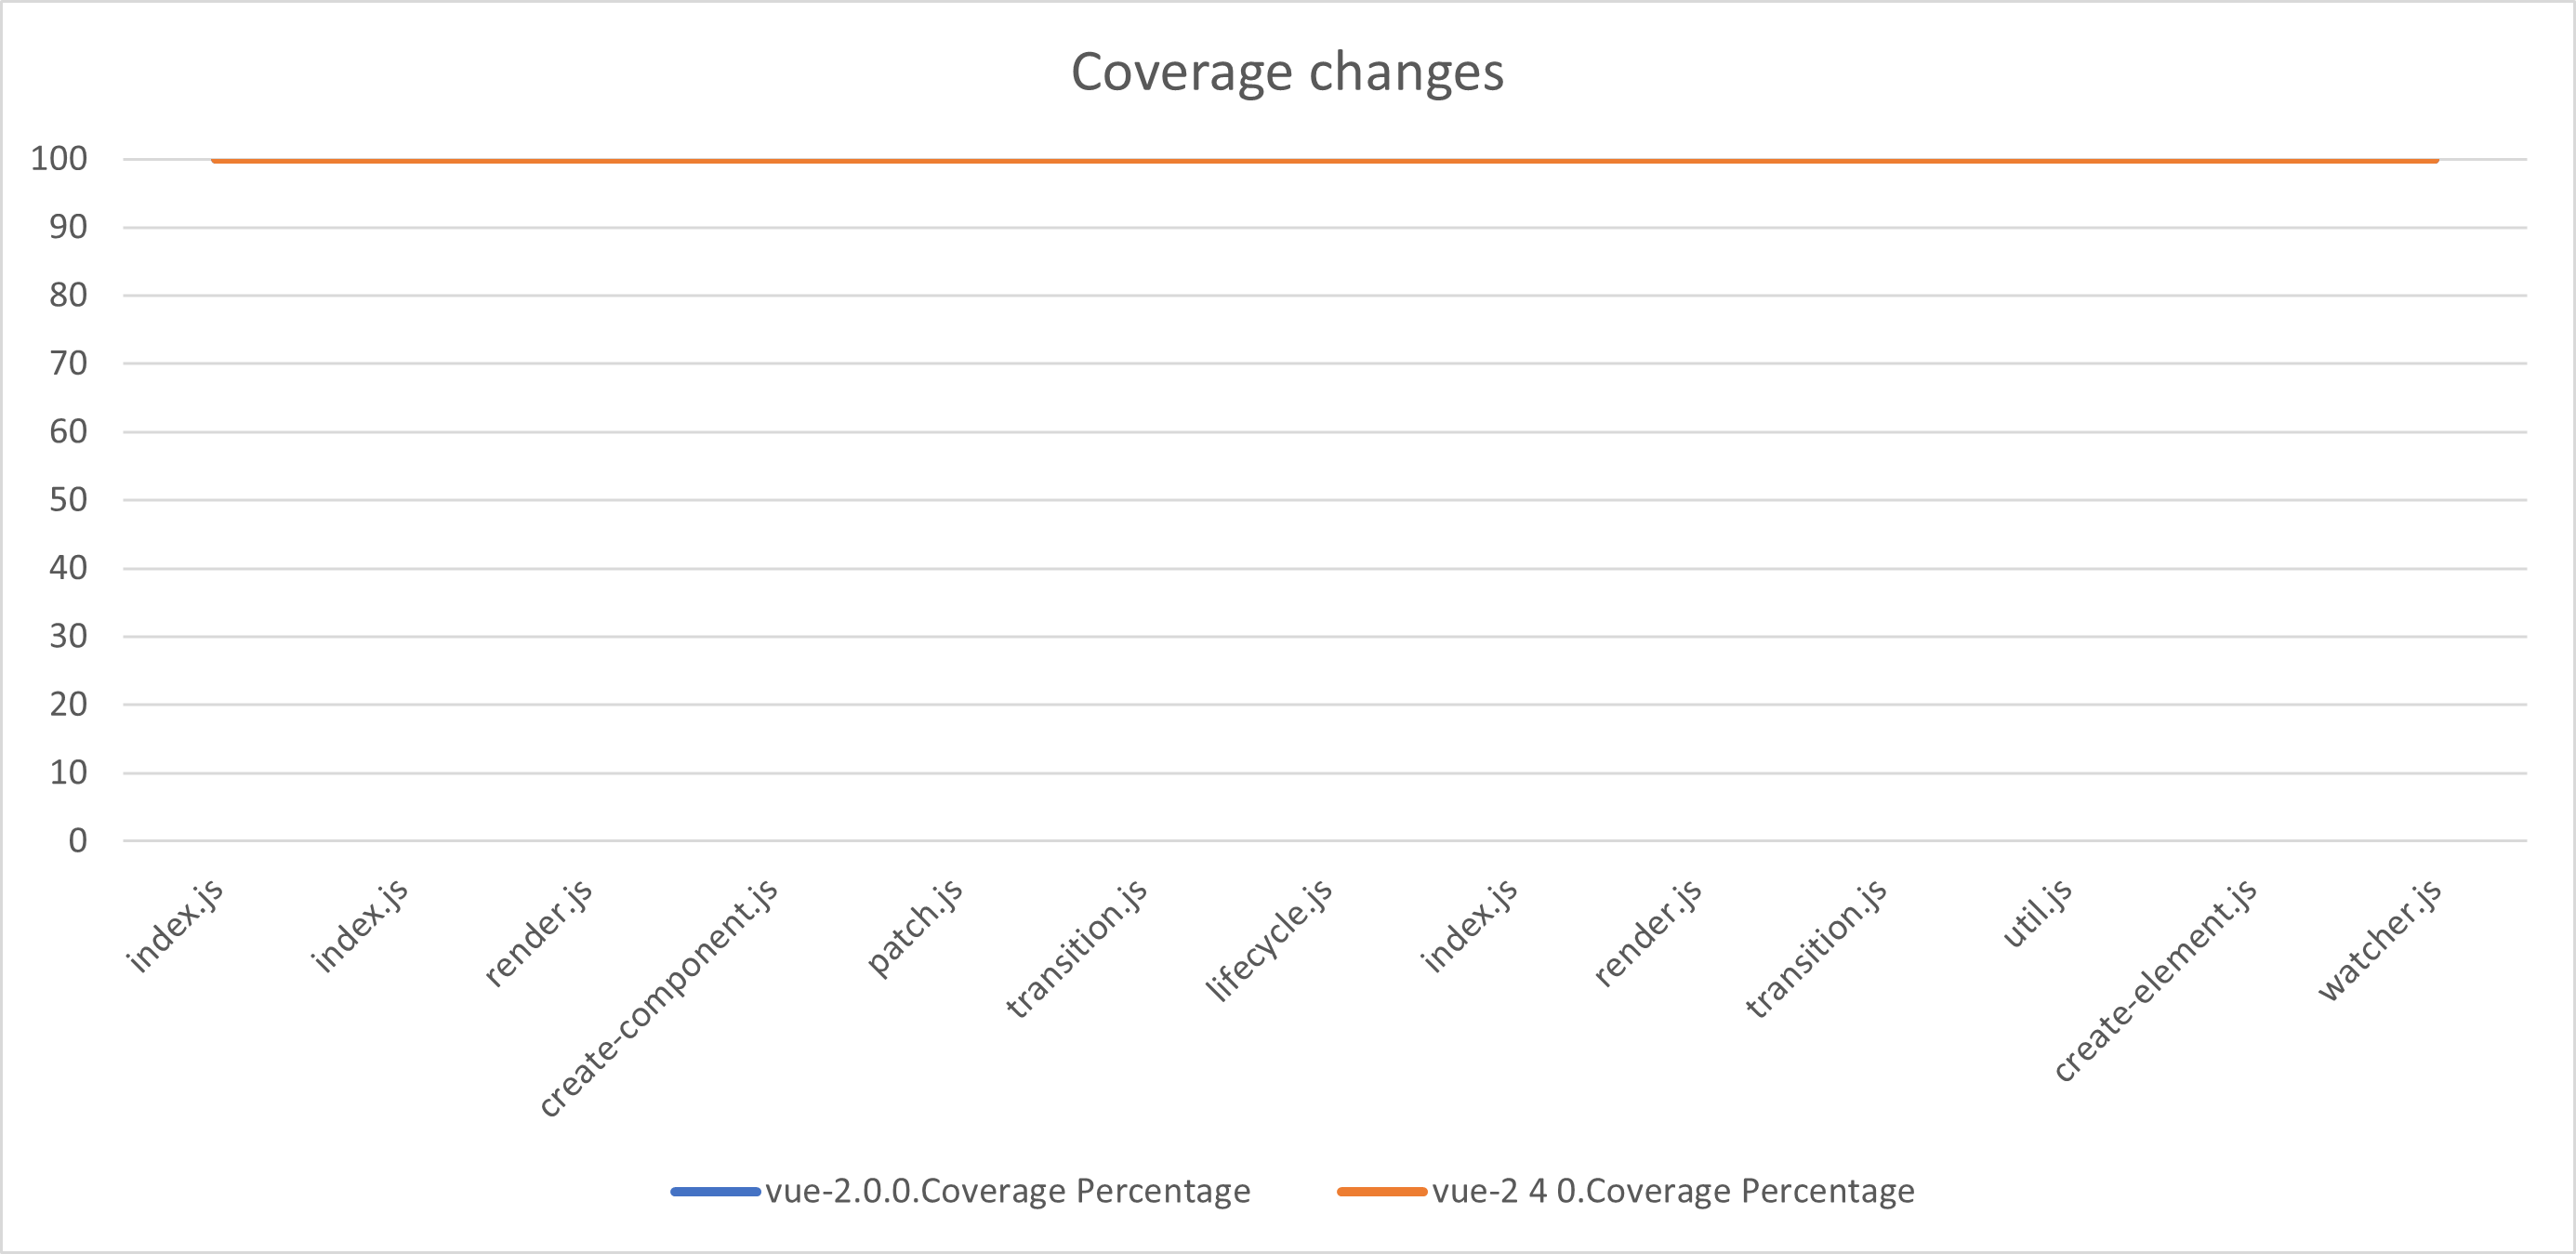
\includegraphics[width=1\textwidth]{images/vue/vue-all-coverage.png}
    \caption{A vue projekt teszt coverage-ének változása 3 verzión keresztül}
    \label{fig:vue-all-coverage}
\end{figure}

\subsection{Megfigyelések}

A vue projekt elemzése összességében sok érdekes trendet tárt fel. Láttuk például, hogy a projekt születésétől kezdve gócpontot alkotó \code{compile.js} még egy teljes refactor után is ugyanazokat a mintákat mutatta, mint korábban.

Megfigyeltük továbbá, hogy a projekt elején fennálló módosítási trendek szinte változatlanok maradnak a projekt élettartama során. Ebbe beleértendő az is, hogy új gócpontok nem igazán tudnak kialakulni, a komplexitás lokalitása változatlan marad.

Végül láttuk azt is, hogy a coverage-nek semmilyen moderáló hatása nincs ezekre a negatív trendekre, hiszen a vue projekt gócpontjai kivétel nélkül 100\%-os coverage-el rendelkeznek. Igaz viszont az is, hogy a gócpontok növekedése nem vezetett a coverage romlásához sem.


\section{Moment.js}

A második mélyebben megvizsgált kódbázis a moment.js\footnote{https://momentjs.com/} lesz. A moment éveken át volt a de facto JavaScript-ben írt dátum-idő könyvtár, azonban 2020-ban különböző okoknál fogva a fejlesztése befejeződött.

A moment kódbázisa két szempontból lesz érdekes: egyrészt "késznek" tekinthető, másrészt egy nagyon jól definiált, kis problémát volt hivatott megoldani a kezdetekből.

Ideális esetben a legelső kiadástól lenne érdemes kezdeni az analízist, azonban a moment 1.0 megjelenésekor sem unit tesztek, sem coverage report nem voltak a projekthez, ráadásul a kódbázis egy masszív JavaScript fájl volt. A moment 2.0 megjelenése azonban viszonylag közel van az 1.0-hoz és a 2.10.5-ös minor release-től kezdve elérhető a coverage report, úgyhogy az lesz a kezdőpont

A \ref{fig:moment-2.10.1-changes} ábrán látható az összes fájl módosítási száma és a fájlokhoz tartozó egyedi szerzők száma. Egy érdekes dolog már most megfigyelhető: ellentétben a vue-val, itt a szórás a különböző fájlok módosítási számai között viszonylag alacsony. Ehhez viszont hozzátartozik a korábban említett 1.0-ás kiadás, ahol a kódbázis egy \code{moment.js} nevű fájl volt, aminek a története egy újraírás miatt nem jelenik meg a 2.x-es kiadásokban.

\begin{figure}[H]
    \centering
    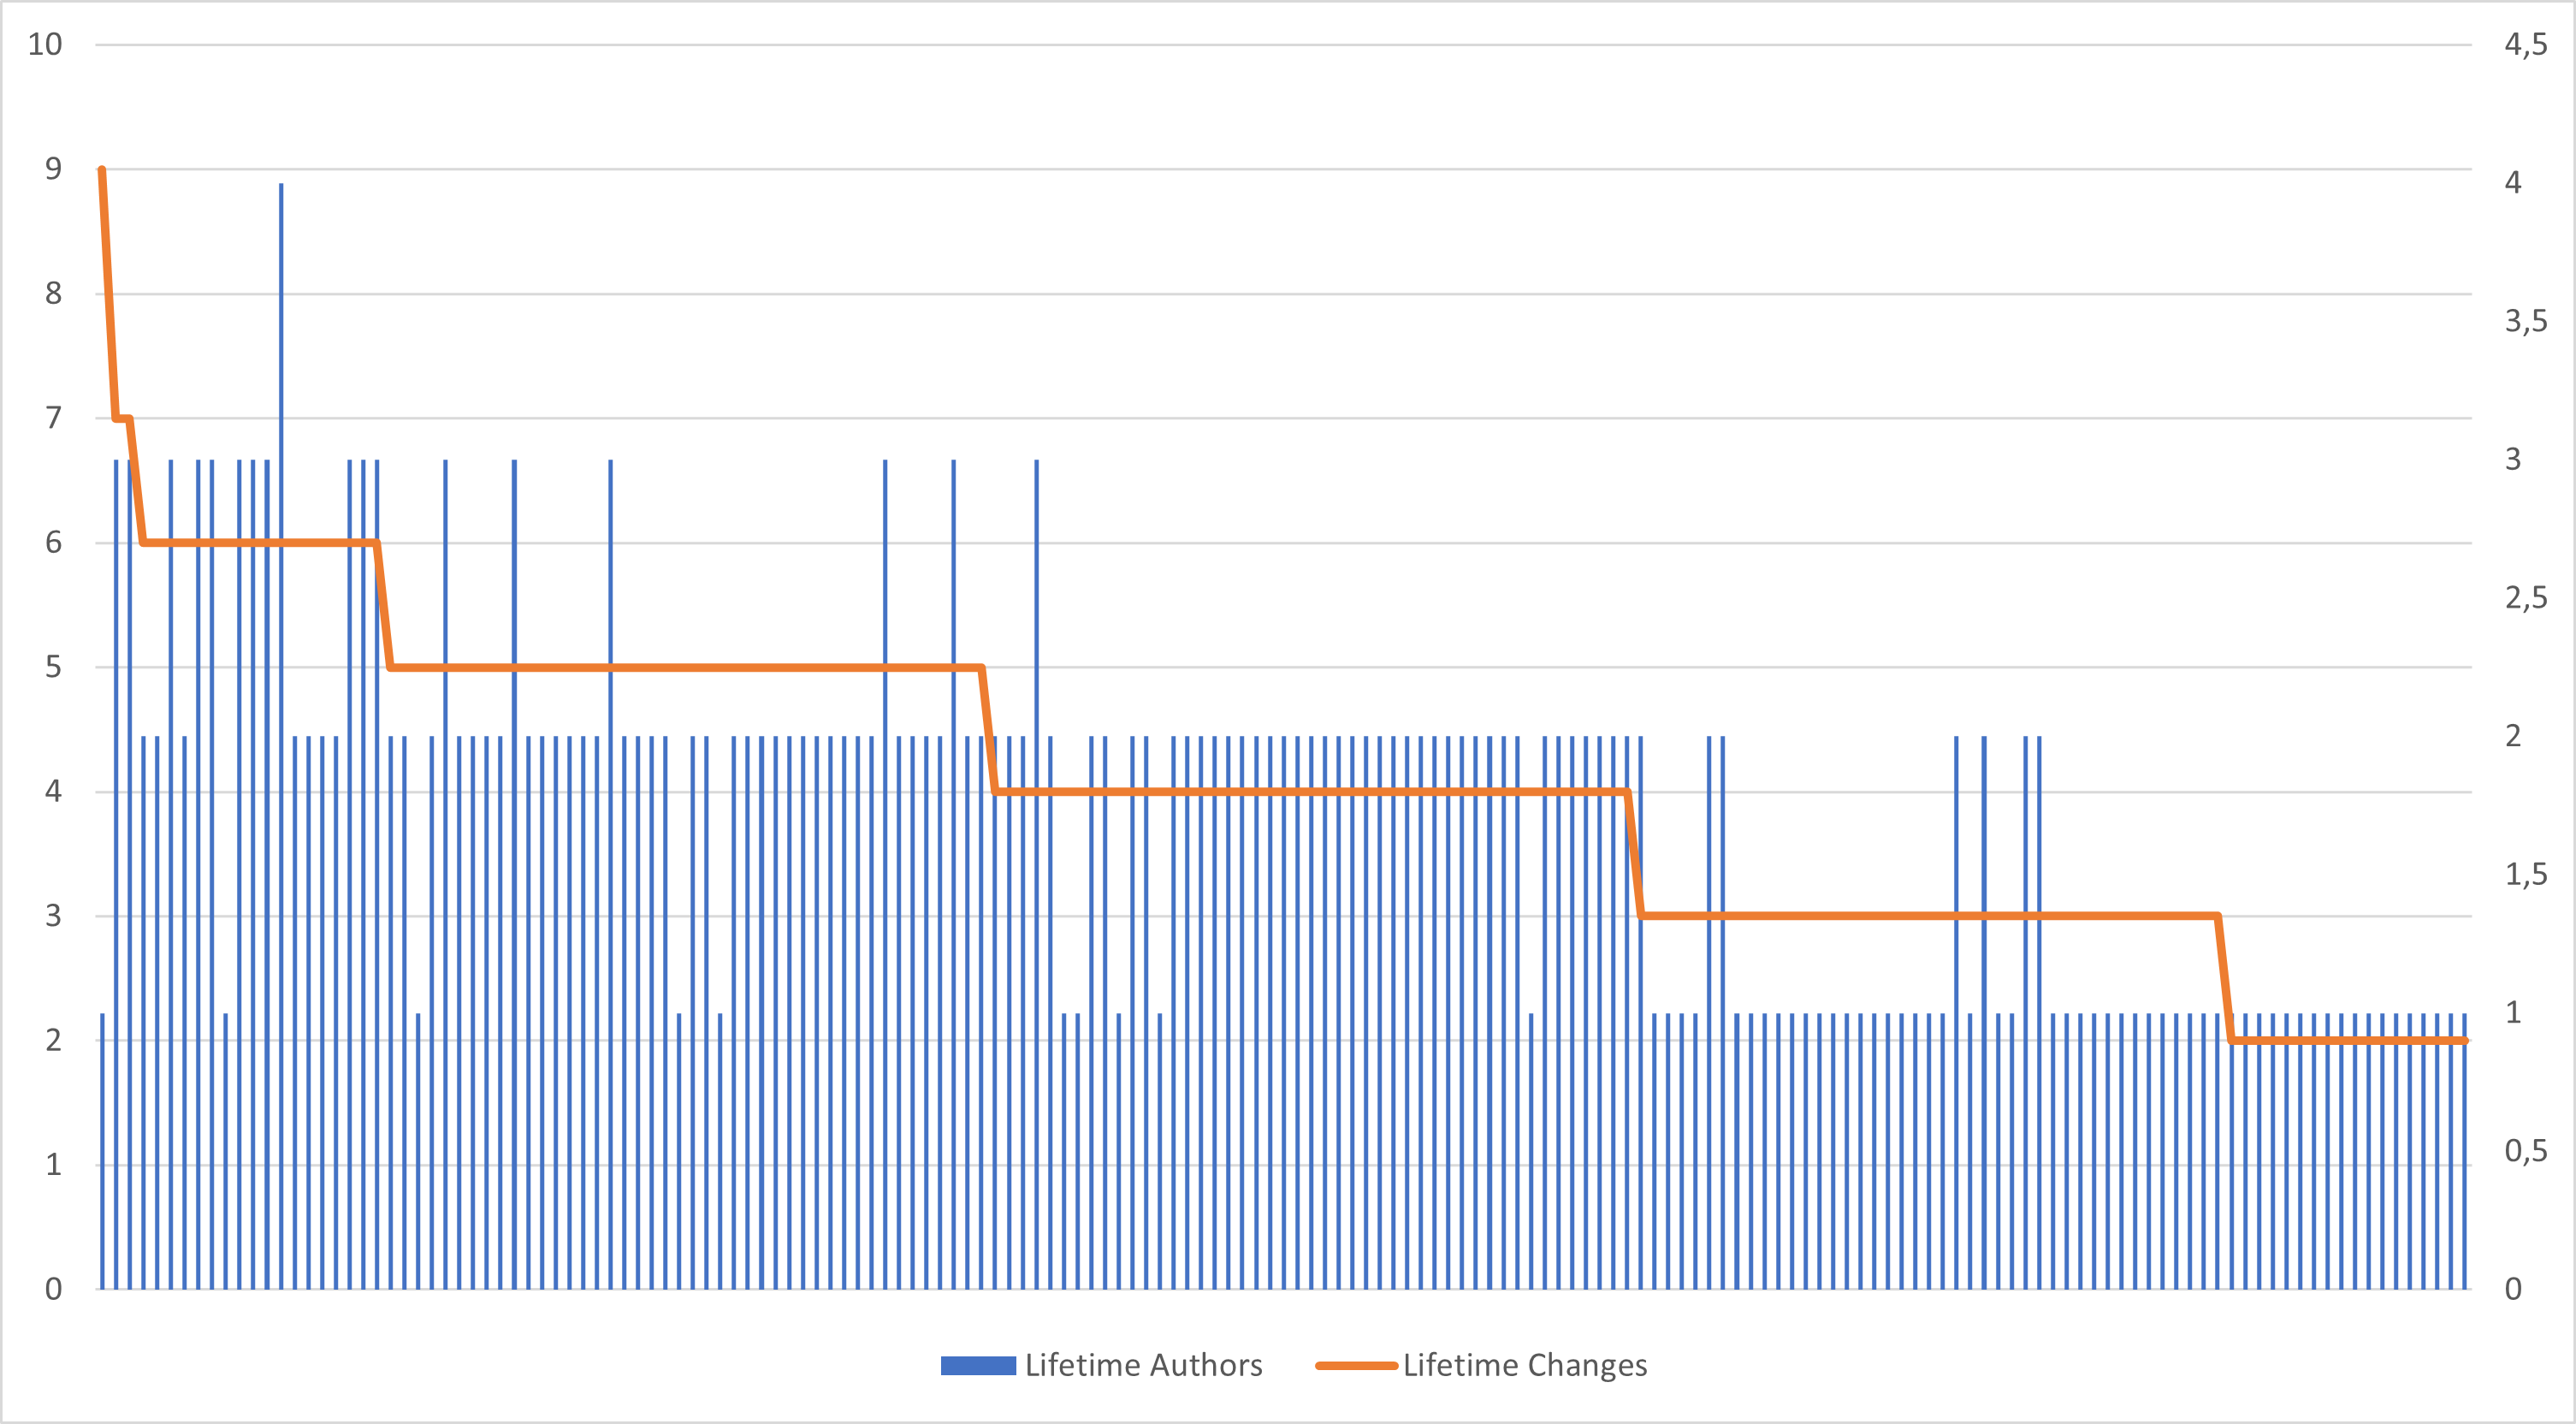
\includegraphics[width=1\textwidth]{images/moment/moment-2.10.5-changes.png}
    \caption{Moment.js 2.10.5-ös kiadásában lévő fájlok módosítási számai}
    \label{fig:moment-2.10.1-changes}
\end{figure}

A \ref{fig:moment-2.10.1-hist} ábrán látható hisztogram jól demonstrálja a kódbázis állapotát a 2.10.5-ös kiadásban. Ugyan technikailag itt is látható az a trend, hogy a fájlok túlnyomó többsége módosítások számát tekintve az alsó 40\%-ban van, azonban itt ez csalóka, hiszen az módosítások számának intervalluma csak 1-től 9-ig terjed.

Egyelőre kijelenthetjük, hogy a moment kódbázisa ezen a ponton kifejezetten lapos a módosítási számok tekintetében, ami ha közelebbről megnézzük a kódbázist akkor érthető is: a logika nagy része a \code{moment.js} fájlban él, különböző kisebb segéd osztályokkal, mint a \code{from-anything.js}, végezetül pedig viszonylag ritkán változtatott lokalizációs fájlokban vannak definiálva a különböző dátum formátumok.

\begin{table}[h]
    \centering
    \begin{tabular}{l|l|l|l|l}
        Filename         & Lifetime Authors & Lifetime Changes & Line \# & Coverage \%       \\ \hline
        moment.js        & 1                & 9                & 68      & 98.02224969097651 \\
        lv.js            & 3                & 7                & 87      & 100               \\
        pt-br.js         & 3                & 7                & 51      & 100               \\
        from-anything.js & 2                & 6                & 96      & 0                 \\
        sl.js            & 2                & 6                & 150     & 90.1639344262295  \\
        day-of-week.js   & 3                & 6                & 134     & 0                 \\
        my.js            & 2                & 6                & 84      & 100               \\
        hu.js            & 3                & 6                & 100     & 92.85714285714286 \\
        hr.js            & 3                & 6                & 131     & 89.1304347826087  \\
        prototype.js     & 1                & 6                & 145     & 0
    \end{tabular}
    \caption{Moment.js 2.10.5}
    \label{tab:moment-2105}
\end{table}

\begin{figure}[H]
    \centering
    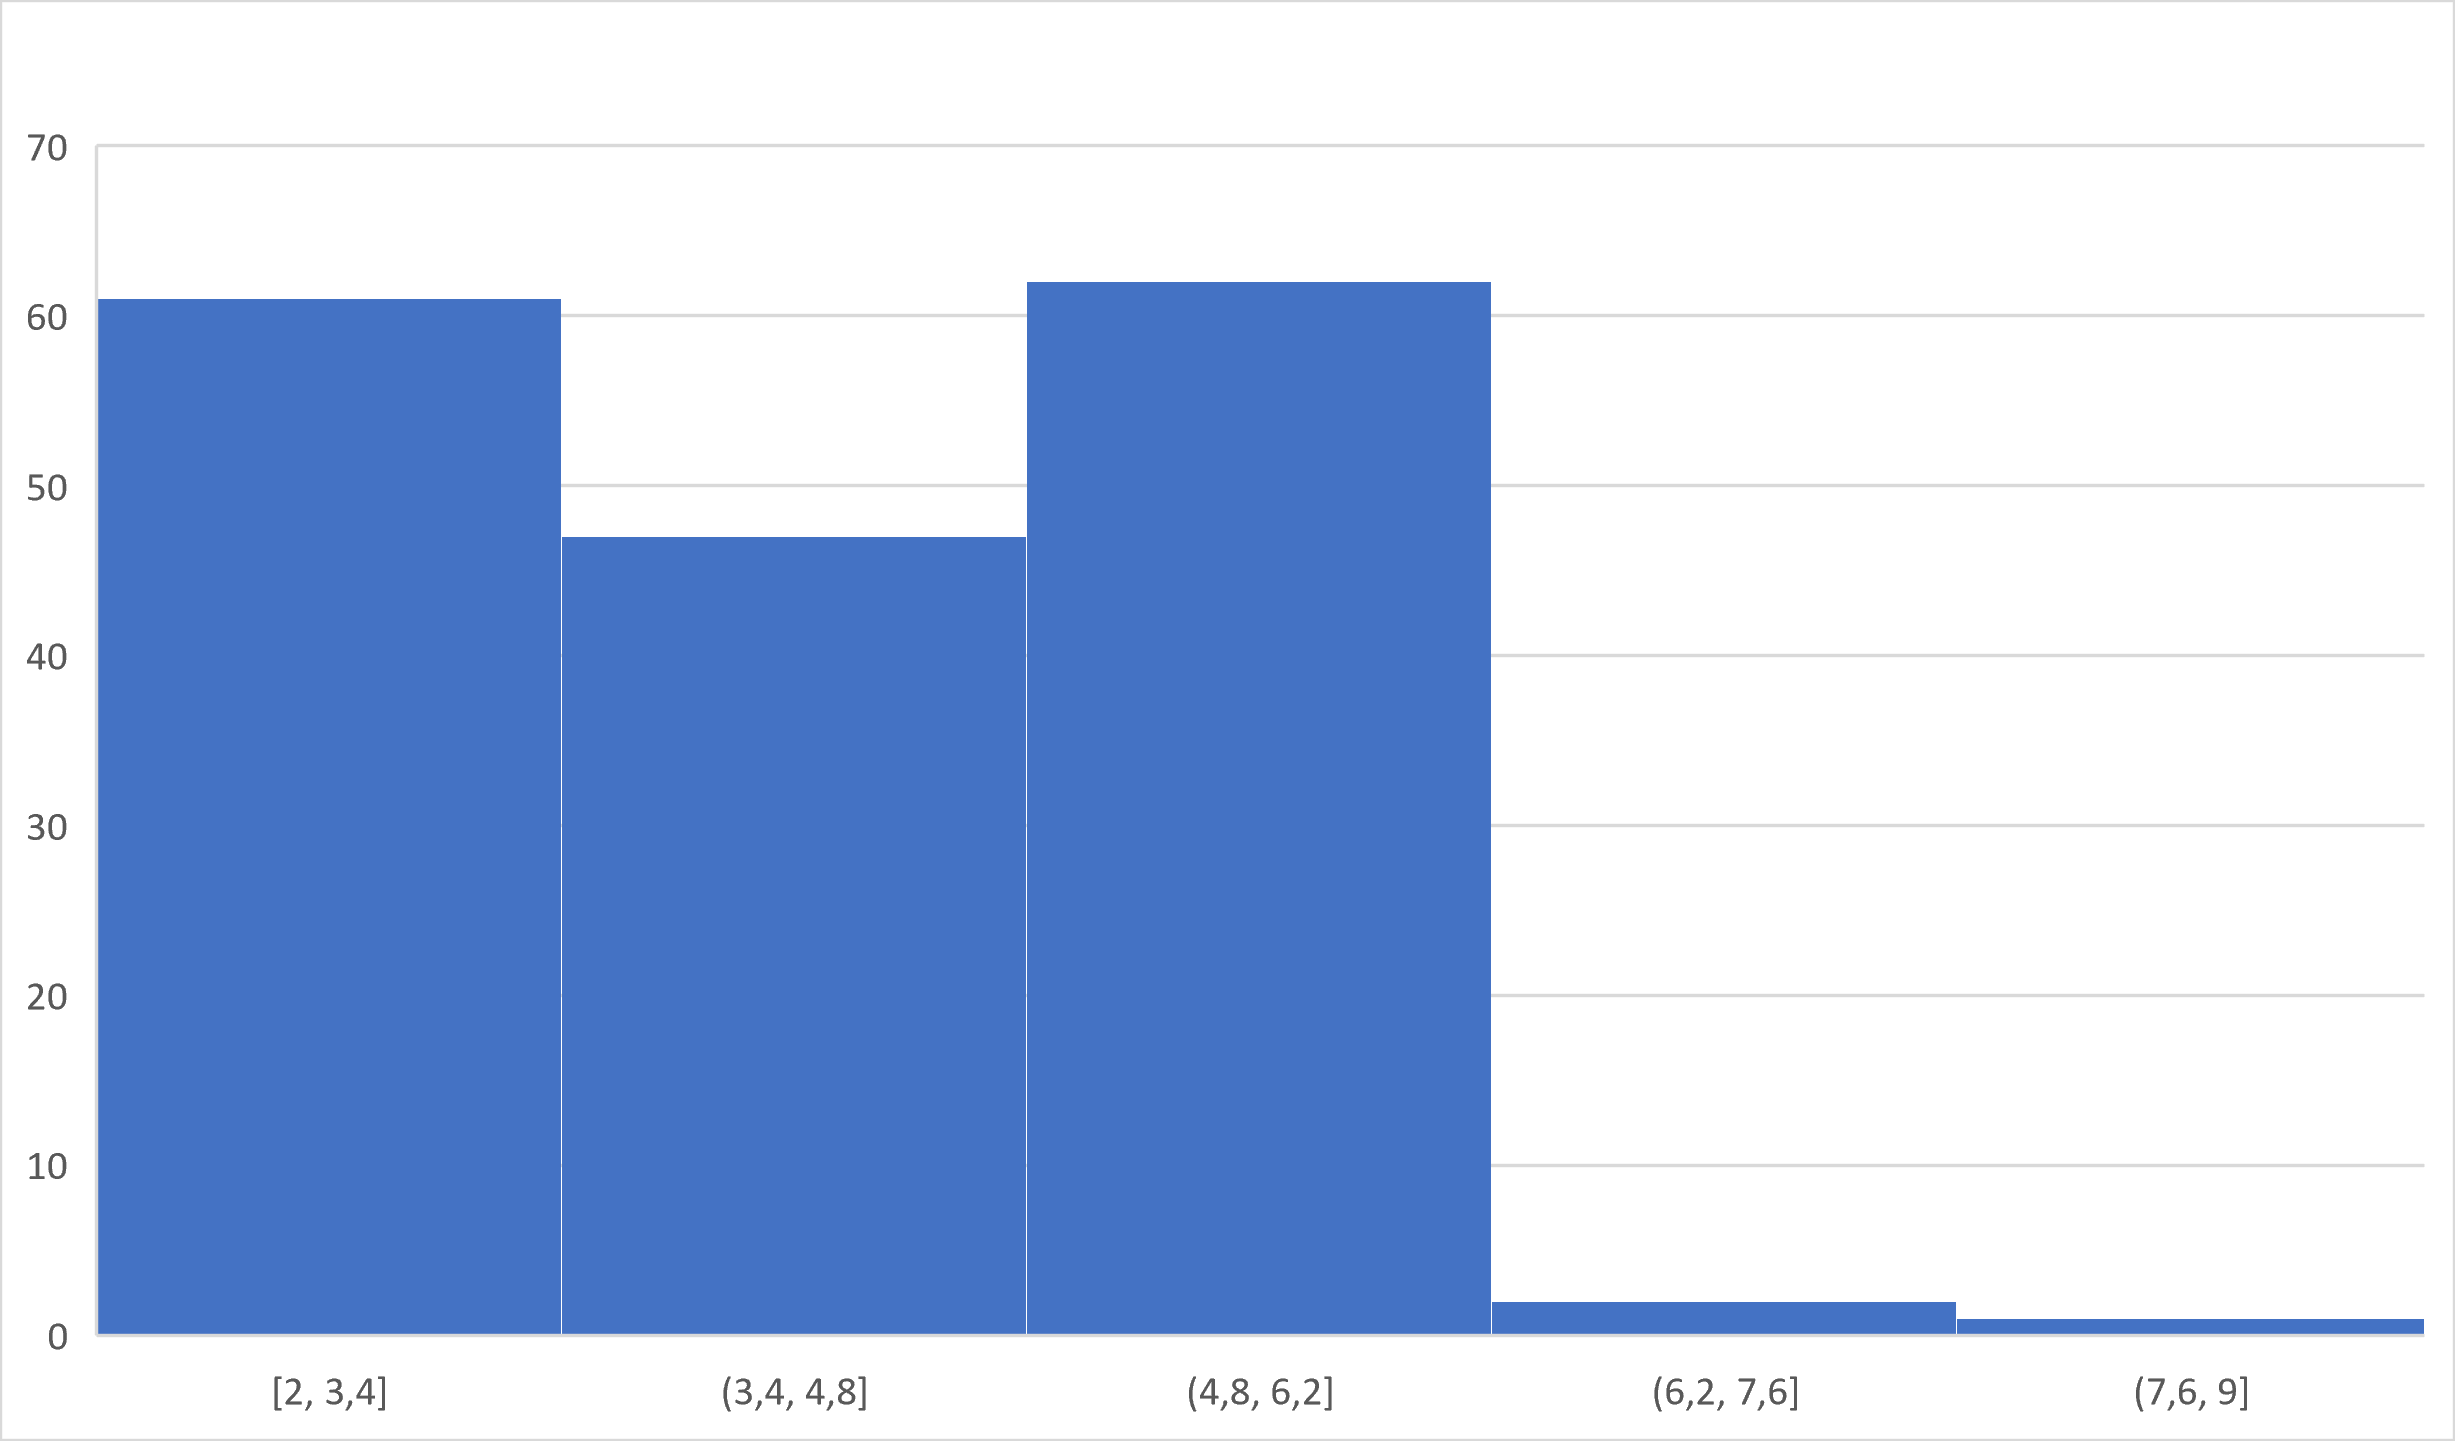
\includegraphics[width=1\textwidth]{images/moment/moment-2.10.5-hist.png}
    \caption{Moment.js 2.10.5-ös kiadásában lévő fájlok módosítási számainak hisztogramja}
    \label{fig:moment-2.10.1-hist}
\end{figure}

Ugorjunk az időben a 2.20.1-es verzióhoz tartozó snapshot-ra, aminek a részletei a \ref{tab:moment-2.20.1} táblázatban láthatóak. Az ebből készített \ref{fig:moment-2.20.1-changes} ábra már jobban hasonlít a vue-nál látottakhoz: változtatások számának tekintetében polarizálódtak a fájlok néhány módosítási gócpont köré. A korábban már látott \code{moment.js} lett az egyik gócpont, illetve kiemelendő még a \code{from-string.js} segéd osztály. A \ref{fig:fig:moment-2.20.1-hist} ábrán is az látszik, hogy közelebb került a moment kódbázisa a korábban látottakhoz.

\begin{table}[h]
    \centering
    \begin{tabular}{l|l|l|l|l}
        Filename       & Lifetime Authors & Lifetime Changes & Line \# & Coverage \%       \\
        from-string.js & 9                & 41               & 230     & 0                 \\
        moment.js      & 9                & 40               & 95      & 96.01510067114094 \\
        month.js       & 11               & 29               & 290     & 59.63855421686747 \\
        locales.js     & 10               & 29               & 186     & 0                 \\
        ru.js          & 9                & 19               & 175     & 90                \\
        day-of-week.js & 7                & 19               & 364     & 0                 \\
        es.js          & 9                & 19               & 83      & 100               \\
        prototype.js   & 7                & 17               & 150     & 50                \\
        from-array.js  & 7                & 16               & 147     & 0
    \end{tabular}
    \caption{Moment.js 2.20.1}
    \label{tab:moment-2.20.1}
\end{table}

\begin{figure}[H]
    \centering
    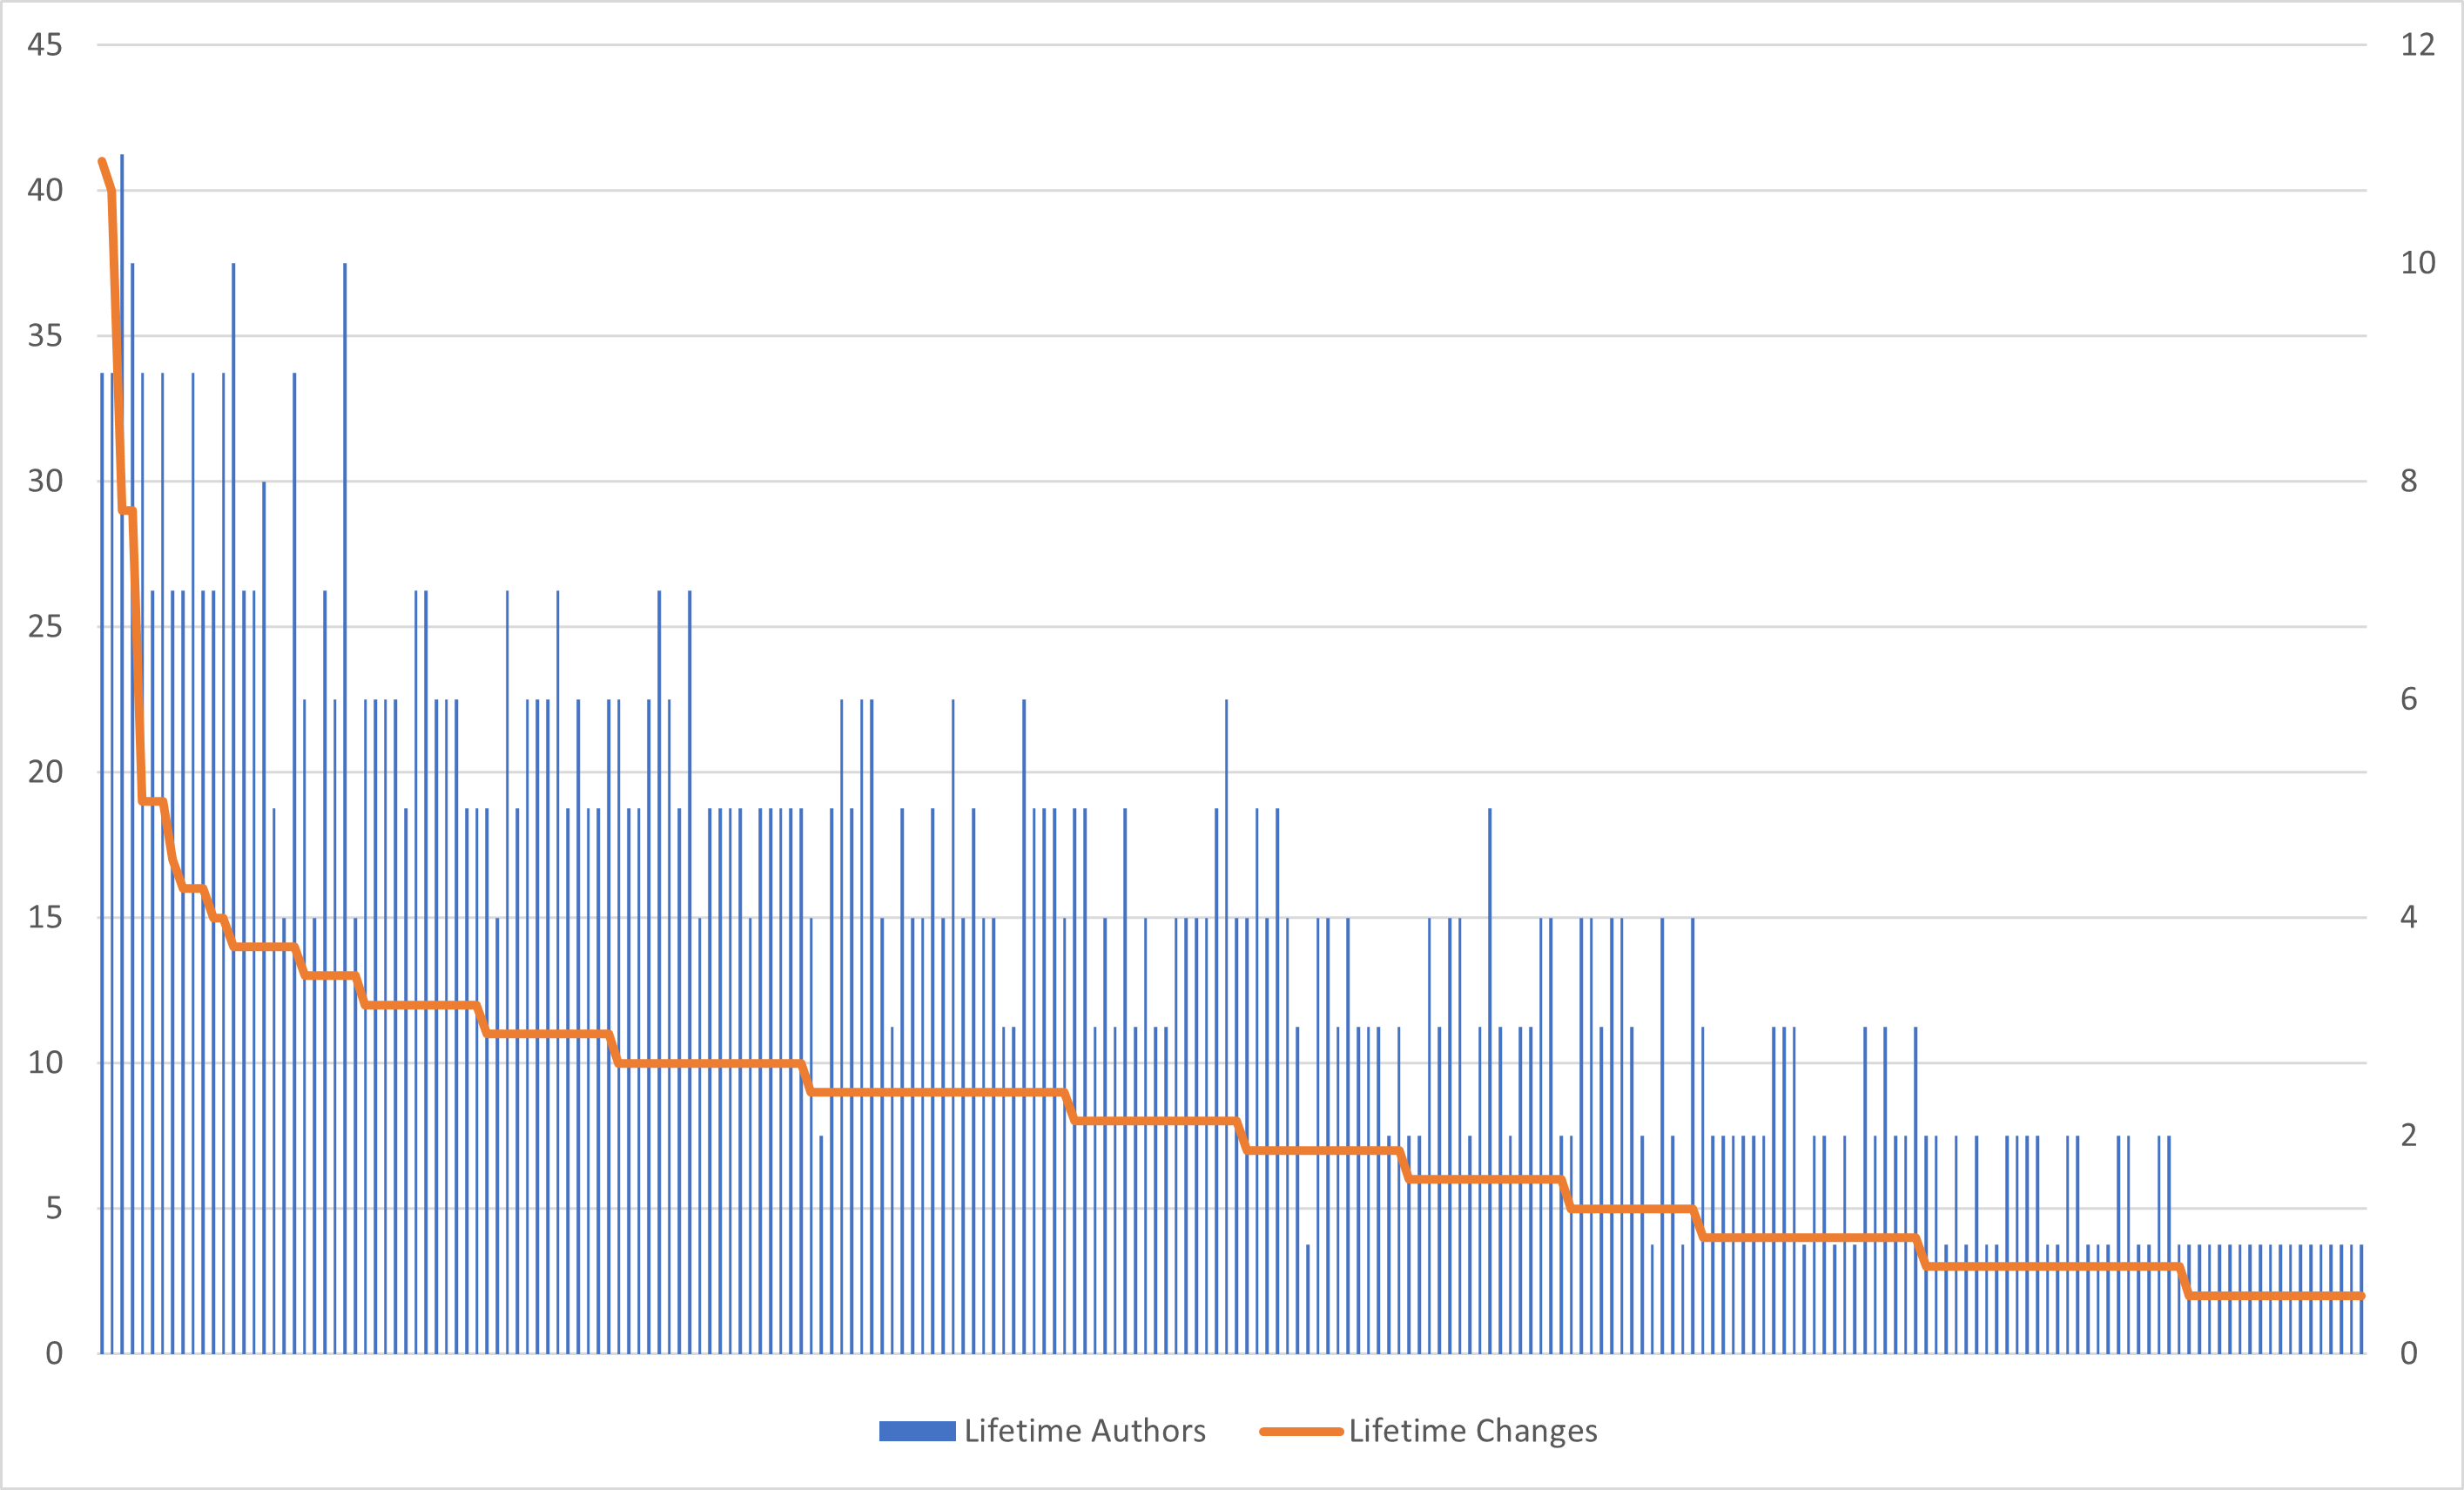
\includegraphics[width=1\textwidth]{images/moment/moment-2.20.5-changes.png}
    \caption{Moment.js 2.20.1-es kiadásában lévő fájlok módosítási számai}
    \label{fig:moment-2.20.1-changes}
\end{figure}

\begin{figure}[H]
    \centering
    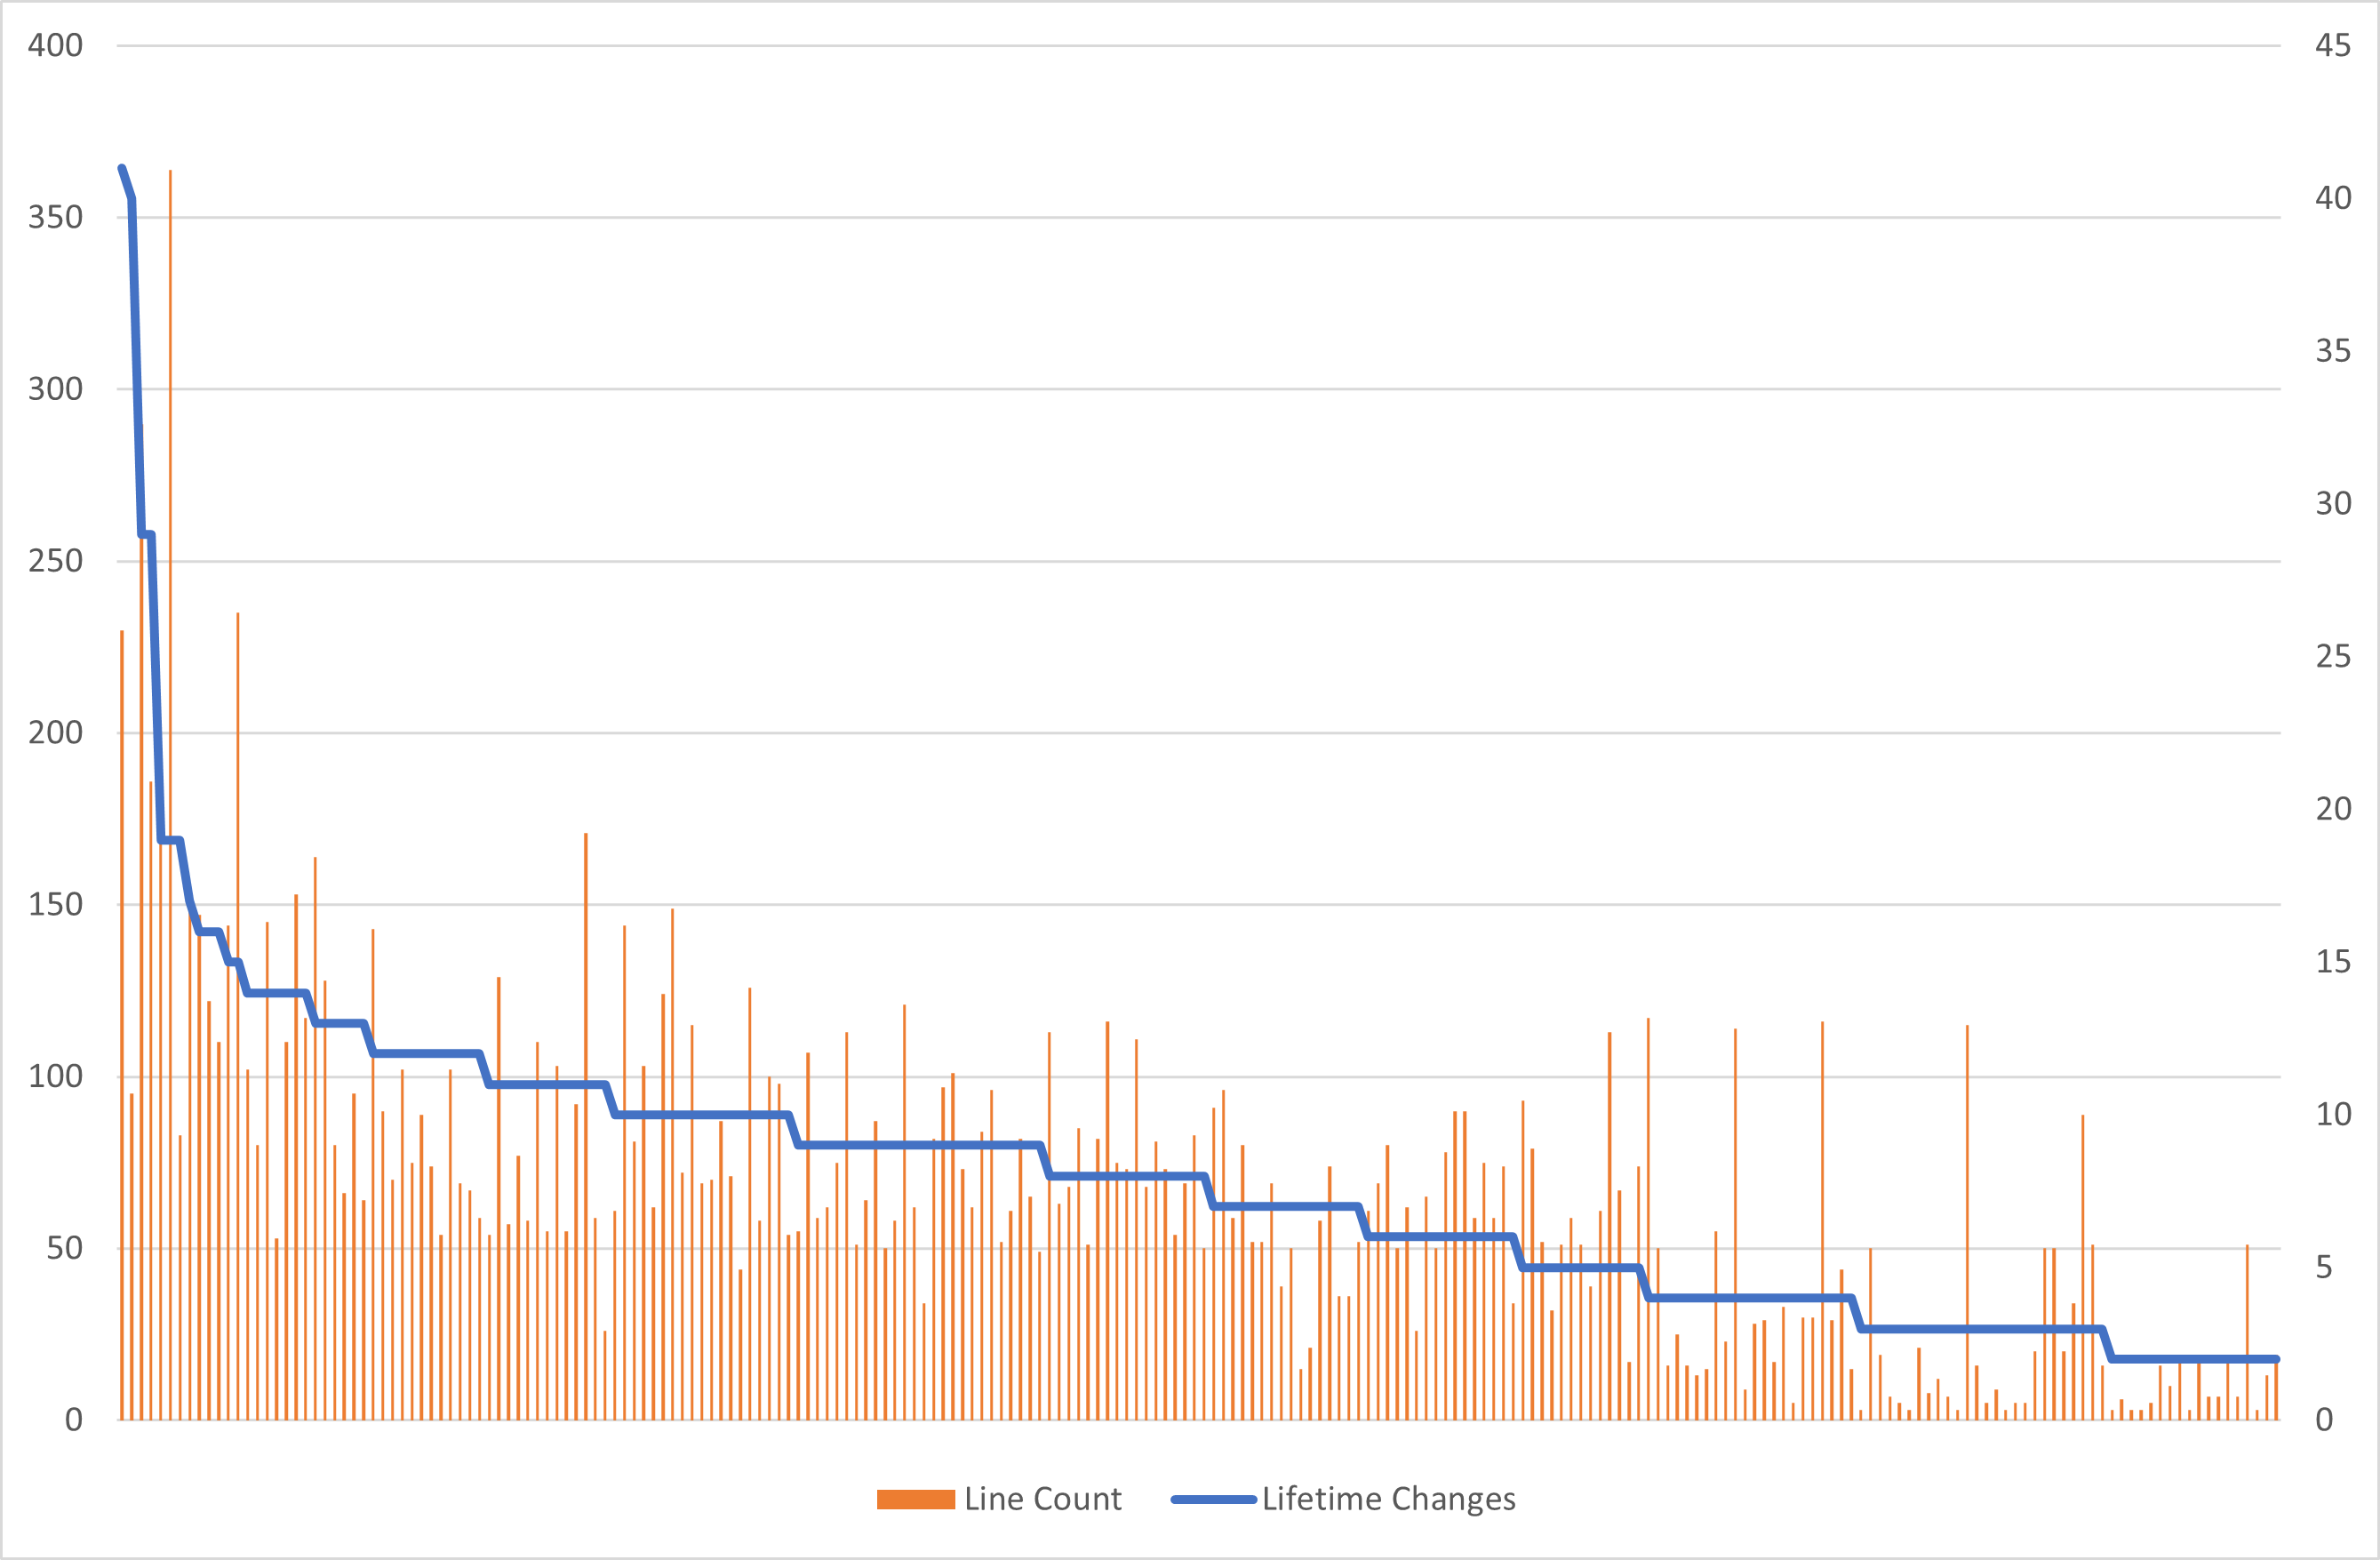
\includegraphics[width=1\textwidth]{images/moment/moment-2.20.5-auth.png}
    \caption{Moment.js 2.20.1-es kiadásában lévő fájlok módosítási számai és egyedi szerzőinek száma}
    \label{fig:moment-2.20.1-auth}
\end{figure}

\begin{figure}[H]
    \centering
    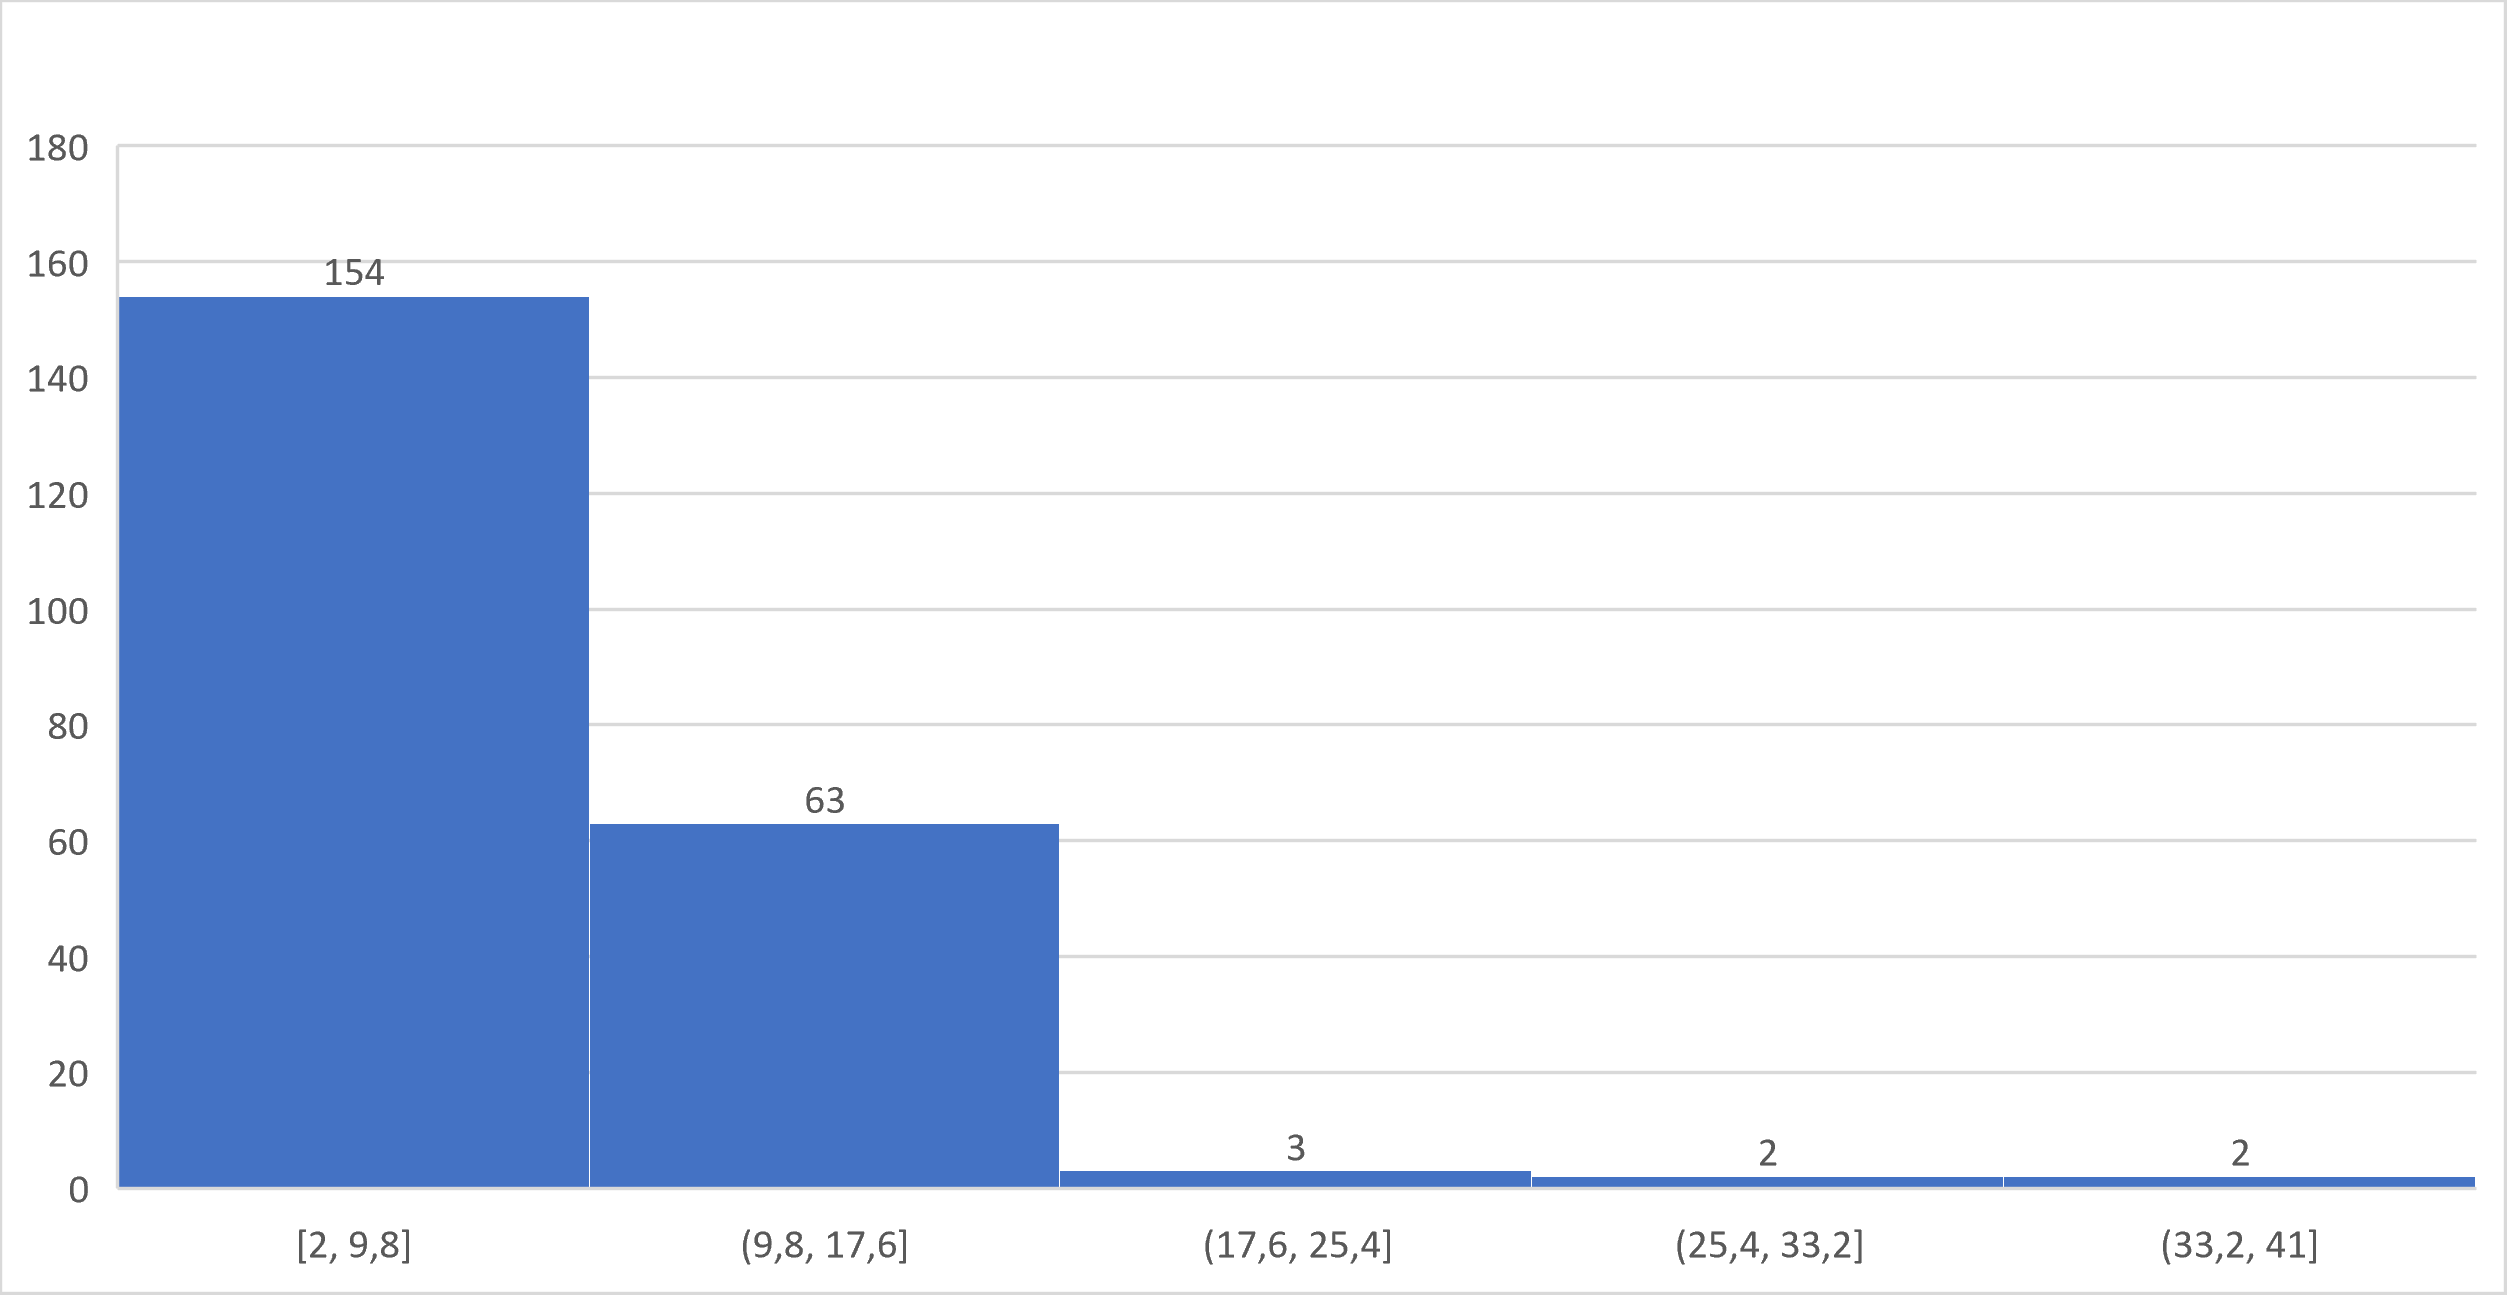
\includegraphics[width=1\textwidth]{images/moment/moment-2.20.5-hist.png}
    \caption{Moment.js 2.20.1-es kiadásában lévő fájlok módosítási számainak hisztogramja}
    \label{fig:moment-2.20.1-hist}
\end{figure}

Nézzük meg a moment.js végső kiadásának adatait. Mint látható a \ref{fig:moment-dev-changes} és \ref{fig:moment-dev-hist} ábrákról a kódbázis erőviszonyai nem változtak a végső kiadásban sem, megtartották azokat a trendeket, amikre a 2.20.1-es kiadás alapján számítanánk. A módosítási számok összehasonlítása a \ref{fig:moment-all-changes} ábrán látható: ebből is látszik, hogy a végső kiadás módosítási számai alapján rajzolt vonal közel van a 2.20.1-es adatokban látott trendekhez, de még a 2.10.5-ös verzióban látott viszonylag lapos kódbázis és a végső állapot közötti korreláció is viszonylag magas, 0,663.

\begin{figure}[H]
    \centering
    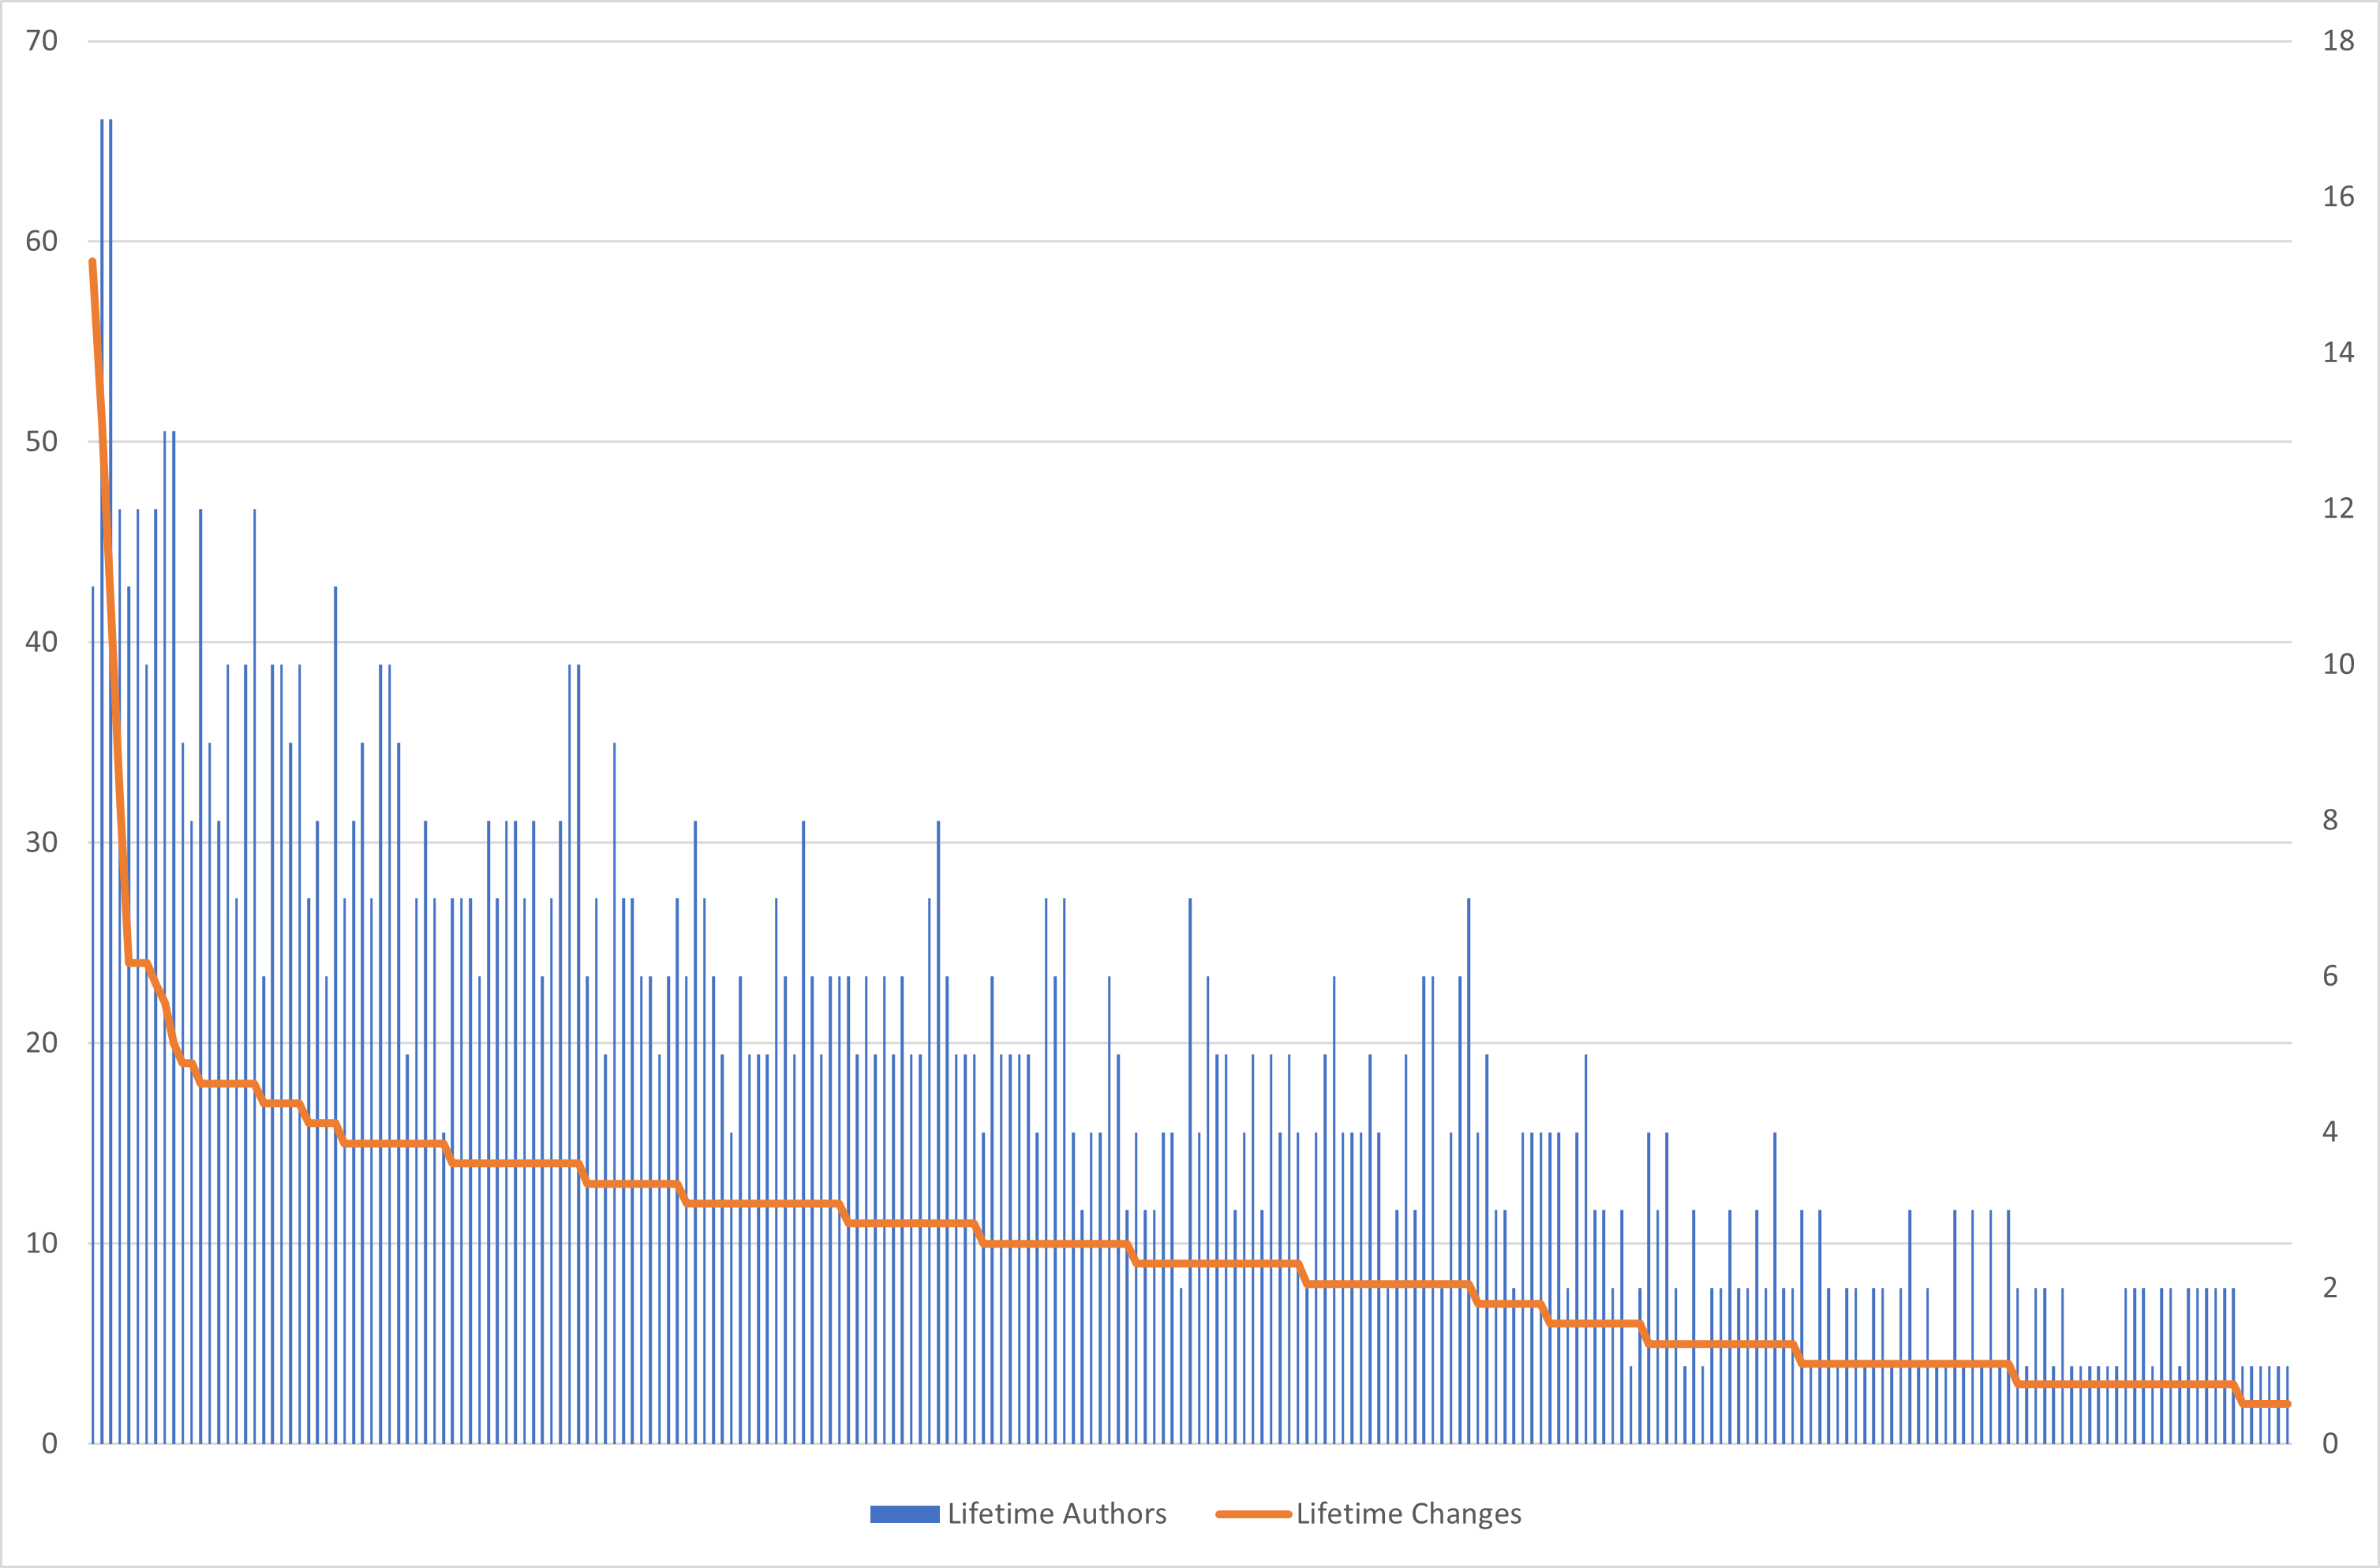
\includegraphics[width=1\textwidth]{images/moment/moment-dev-changes.png}
    \caption{Moment.js legfrisebb és egyben végső kiadásában lévő fájlok módosítási számai}
    \label{fig:moment-dev-changes}
\end{figure}

\begin{figure}[H]
    \centering
    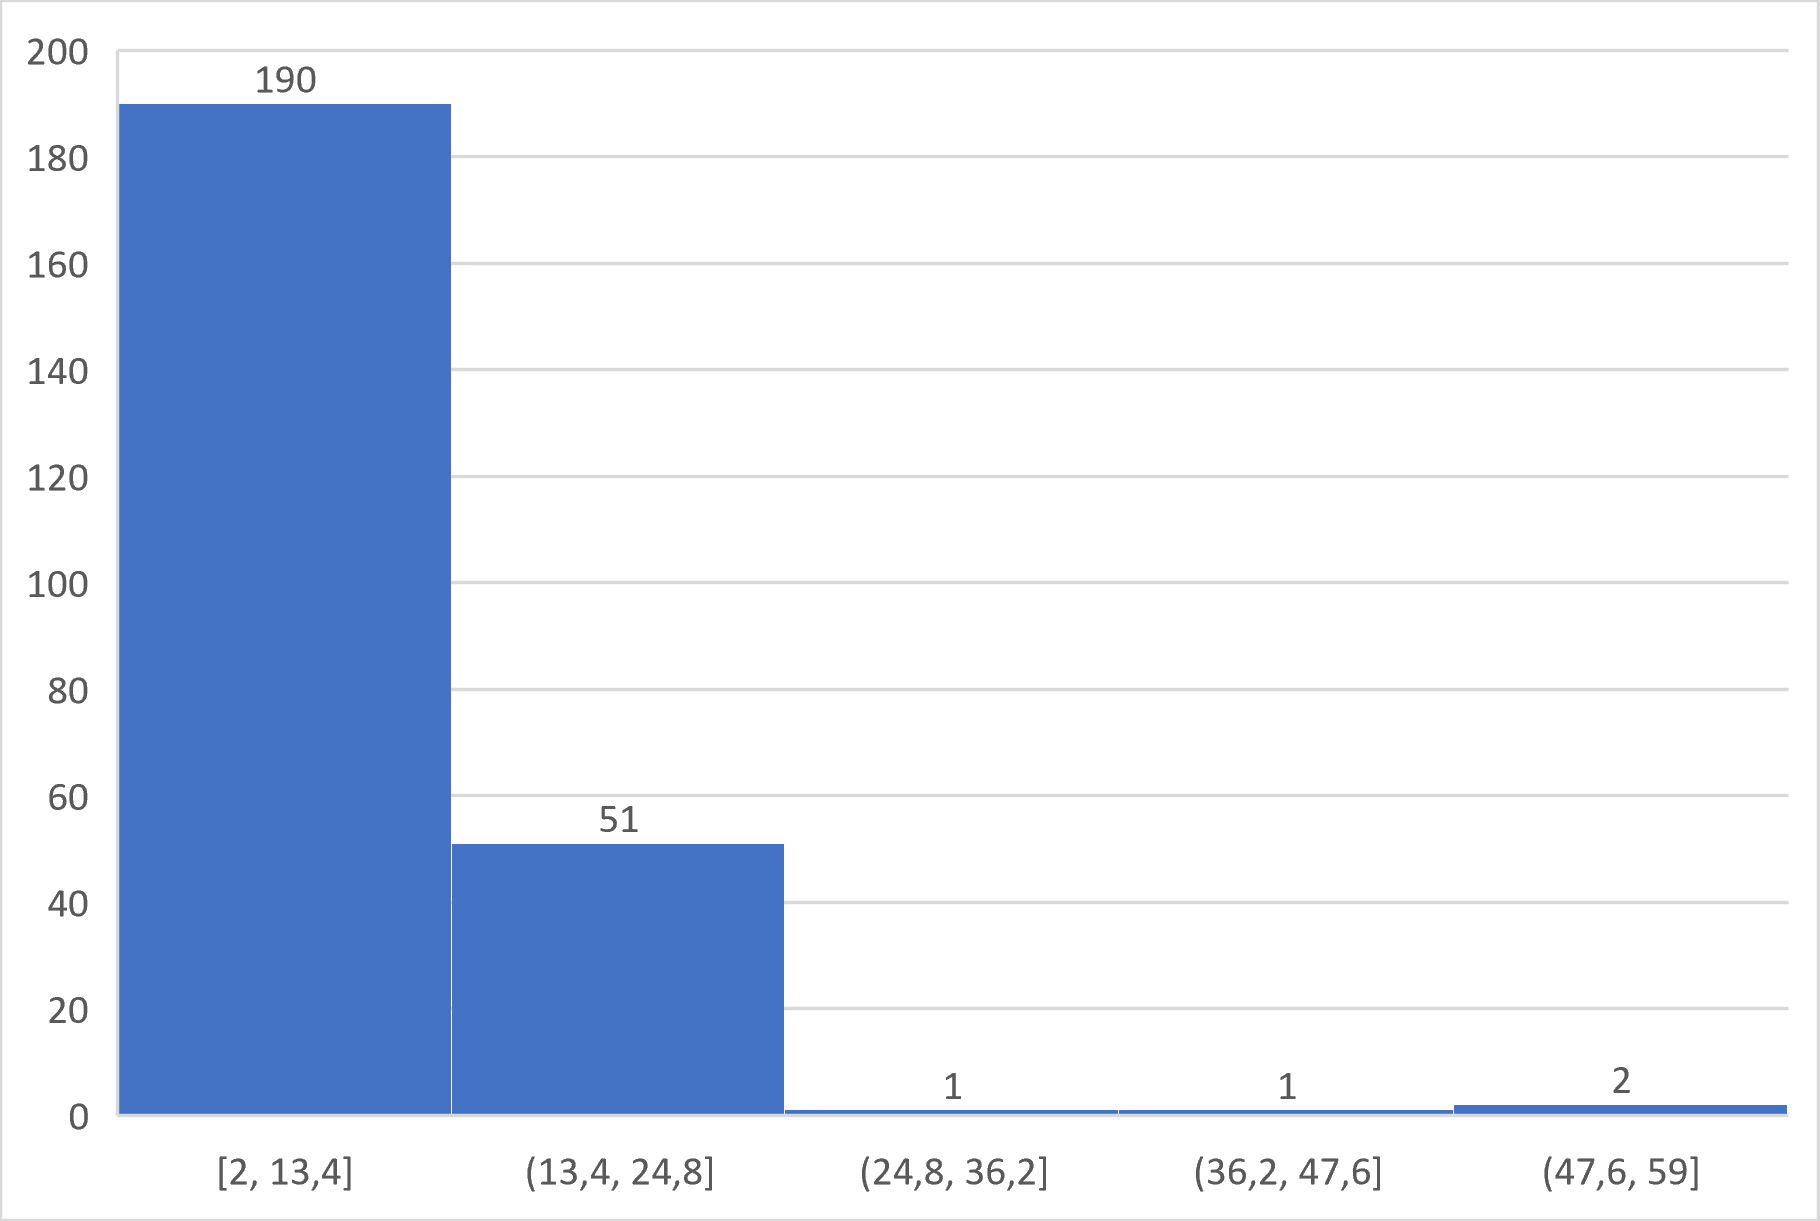
\includegraphics[width=1\textwidth]{images/moment/moment-dev-hist.png}
    \caption{Moment.js legfrisebb és egyben végső kiadásában lévő fájlok módosításinak hisztogramja}
    \label{fig:moment-dev-hist}
\end{figure}

\begin{figure}[H]
    \centering
    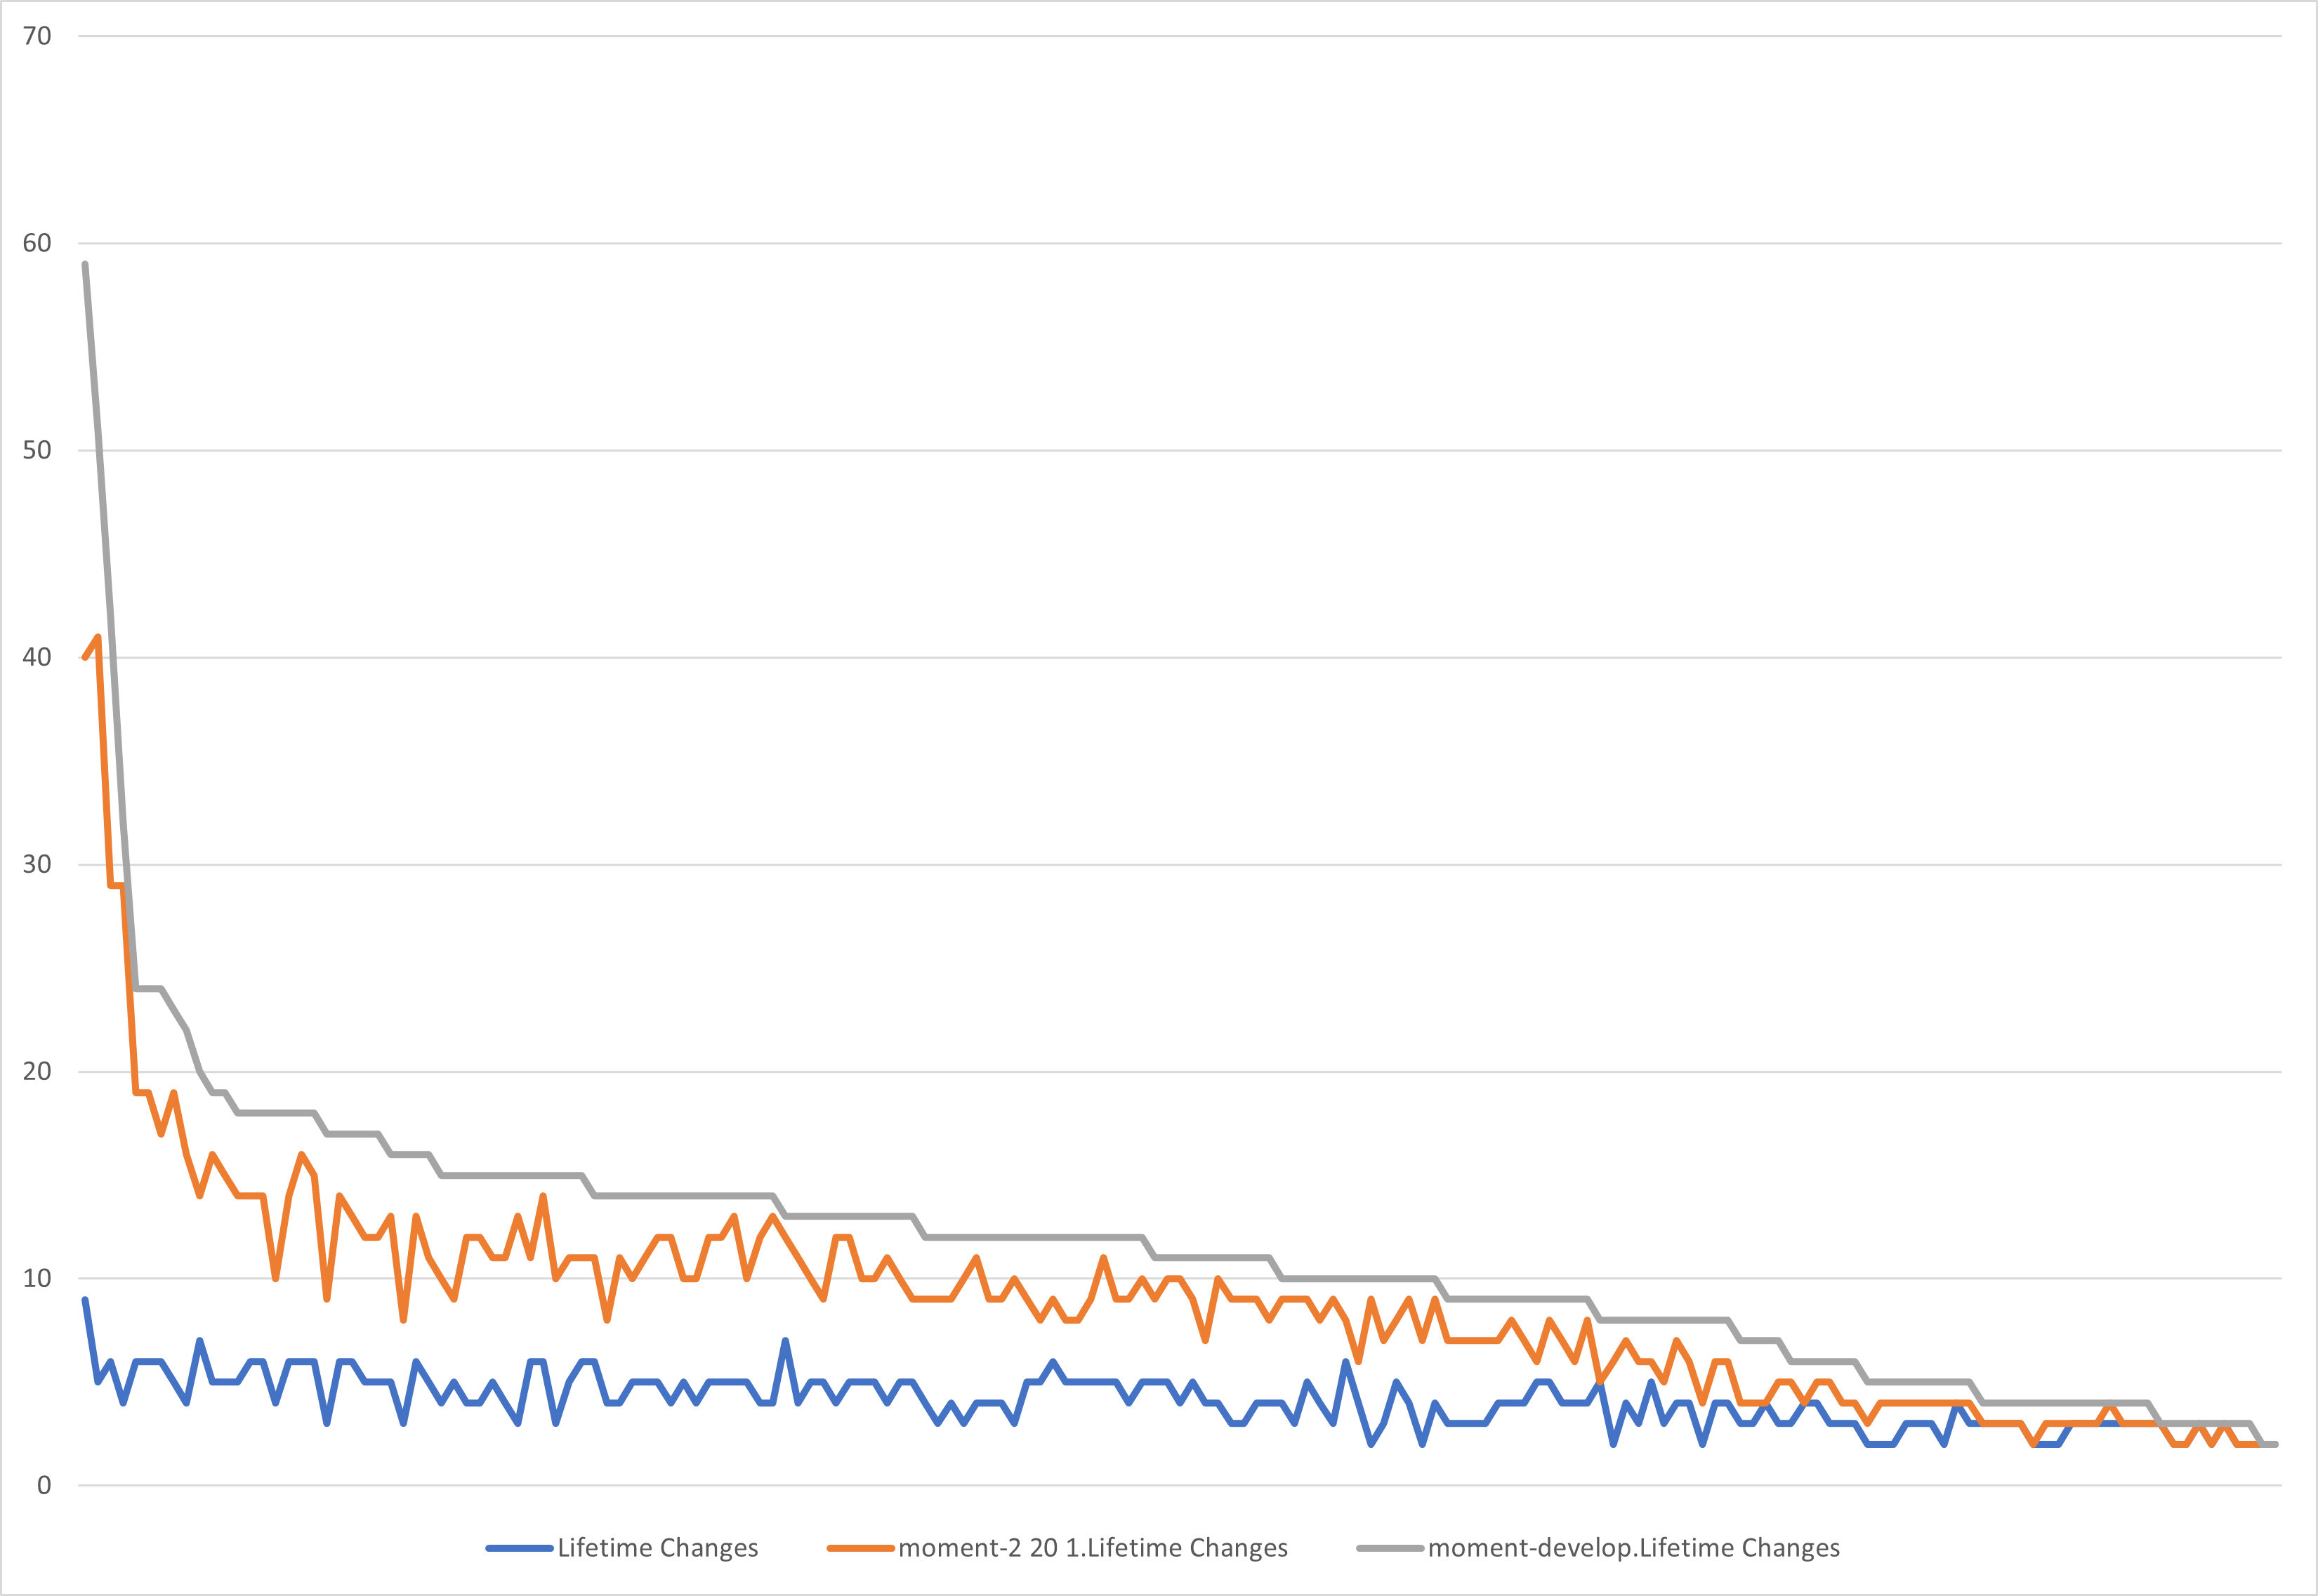
\includegraphics[width=1\textwidth]{images/moment/moment-all-changes.png}
    \caption{Moment.js módosítási számainak alakulása 2.10.5 és a végső kiadás között}
    \label{fig:moment-all-changes}
\end{figure}

Végül érdemes még röviden szót ejteni a coverage trendekről, mivel a moment.js reprezentálja az analízisek között az olyan kódbázist, ahol megkérdőjelezhető a tesztelés mennyisége és minősége.

Leszámítva az olyan anomáliákat, mint a \code{locale.js} és \code{ru.js} esetén eltűnő tesztek a 2.10.5-ös verziót követően, a kódbázis nagy részén

\begin{figure}[H]
    \centering
    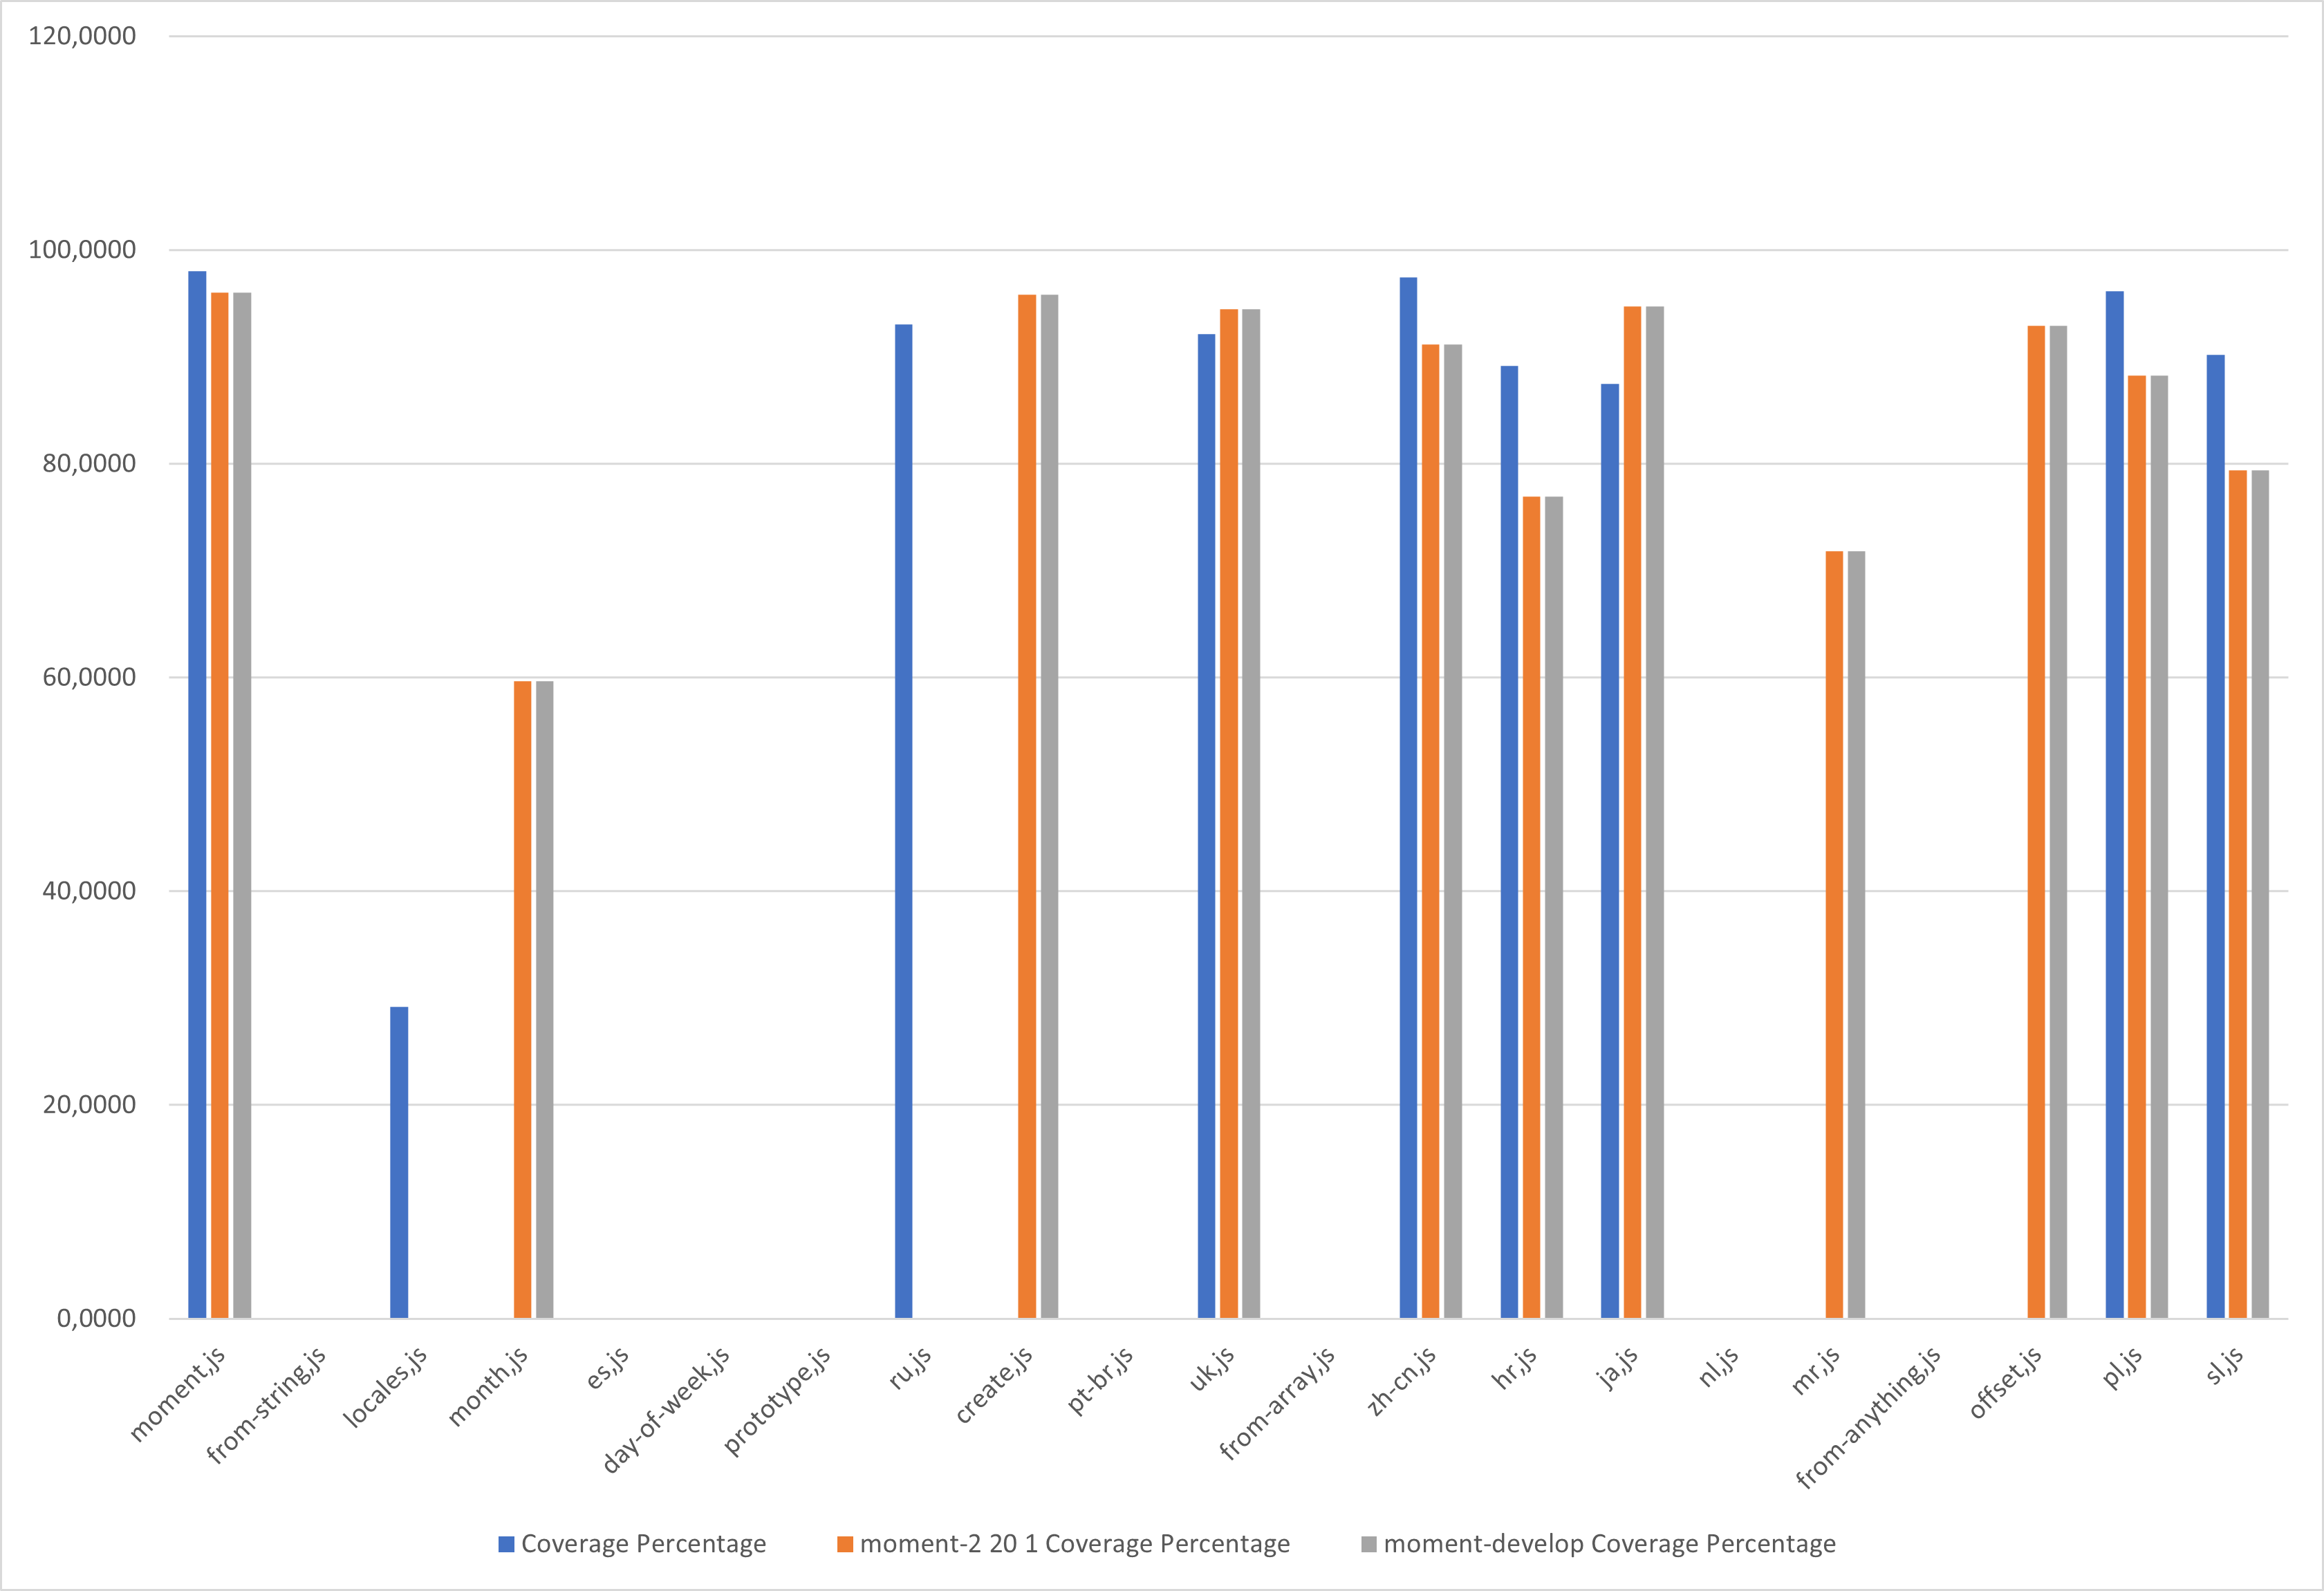
\includegraphics[width=1\textwidth]{images/moment/moment-all-coverage.png}
    \caption{Moment.js test coverage-ének alakulása 2.10.5 és a végső kiadás között}
    \label{fig:moment-all-coverage}
\end{figure}

\begin{figure}[H]
    \centering
    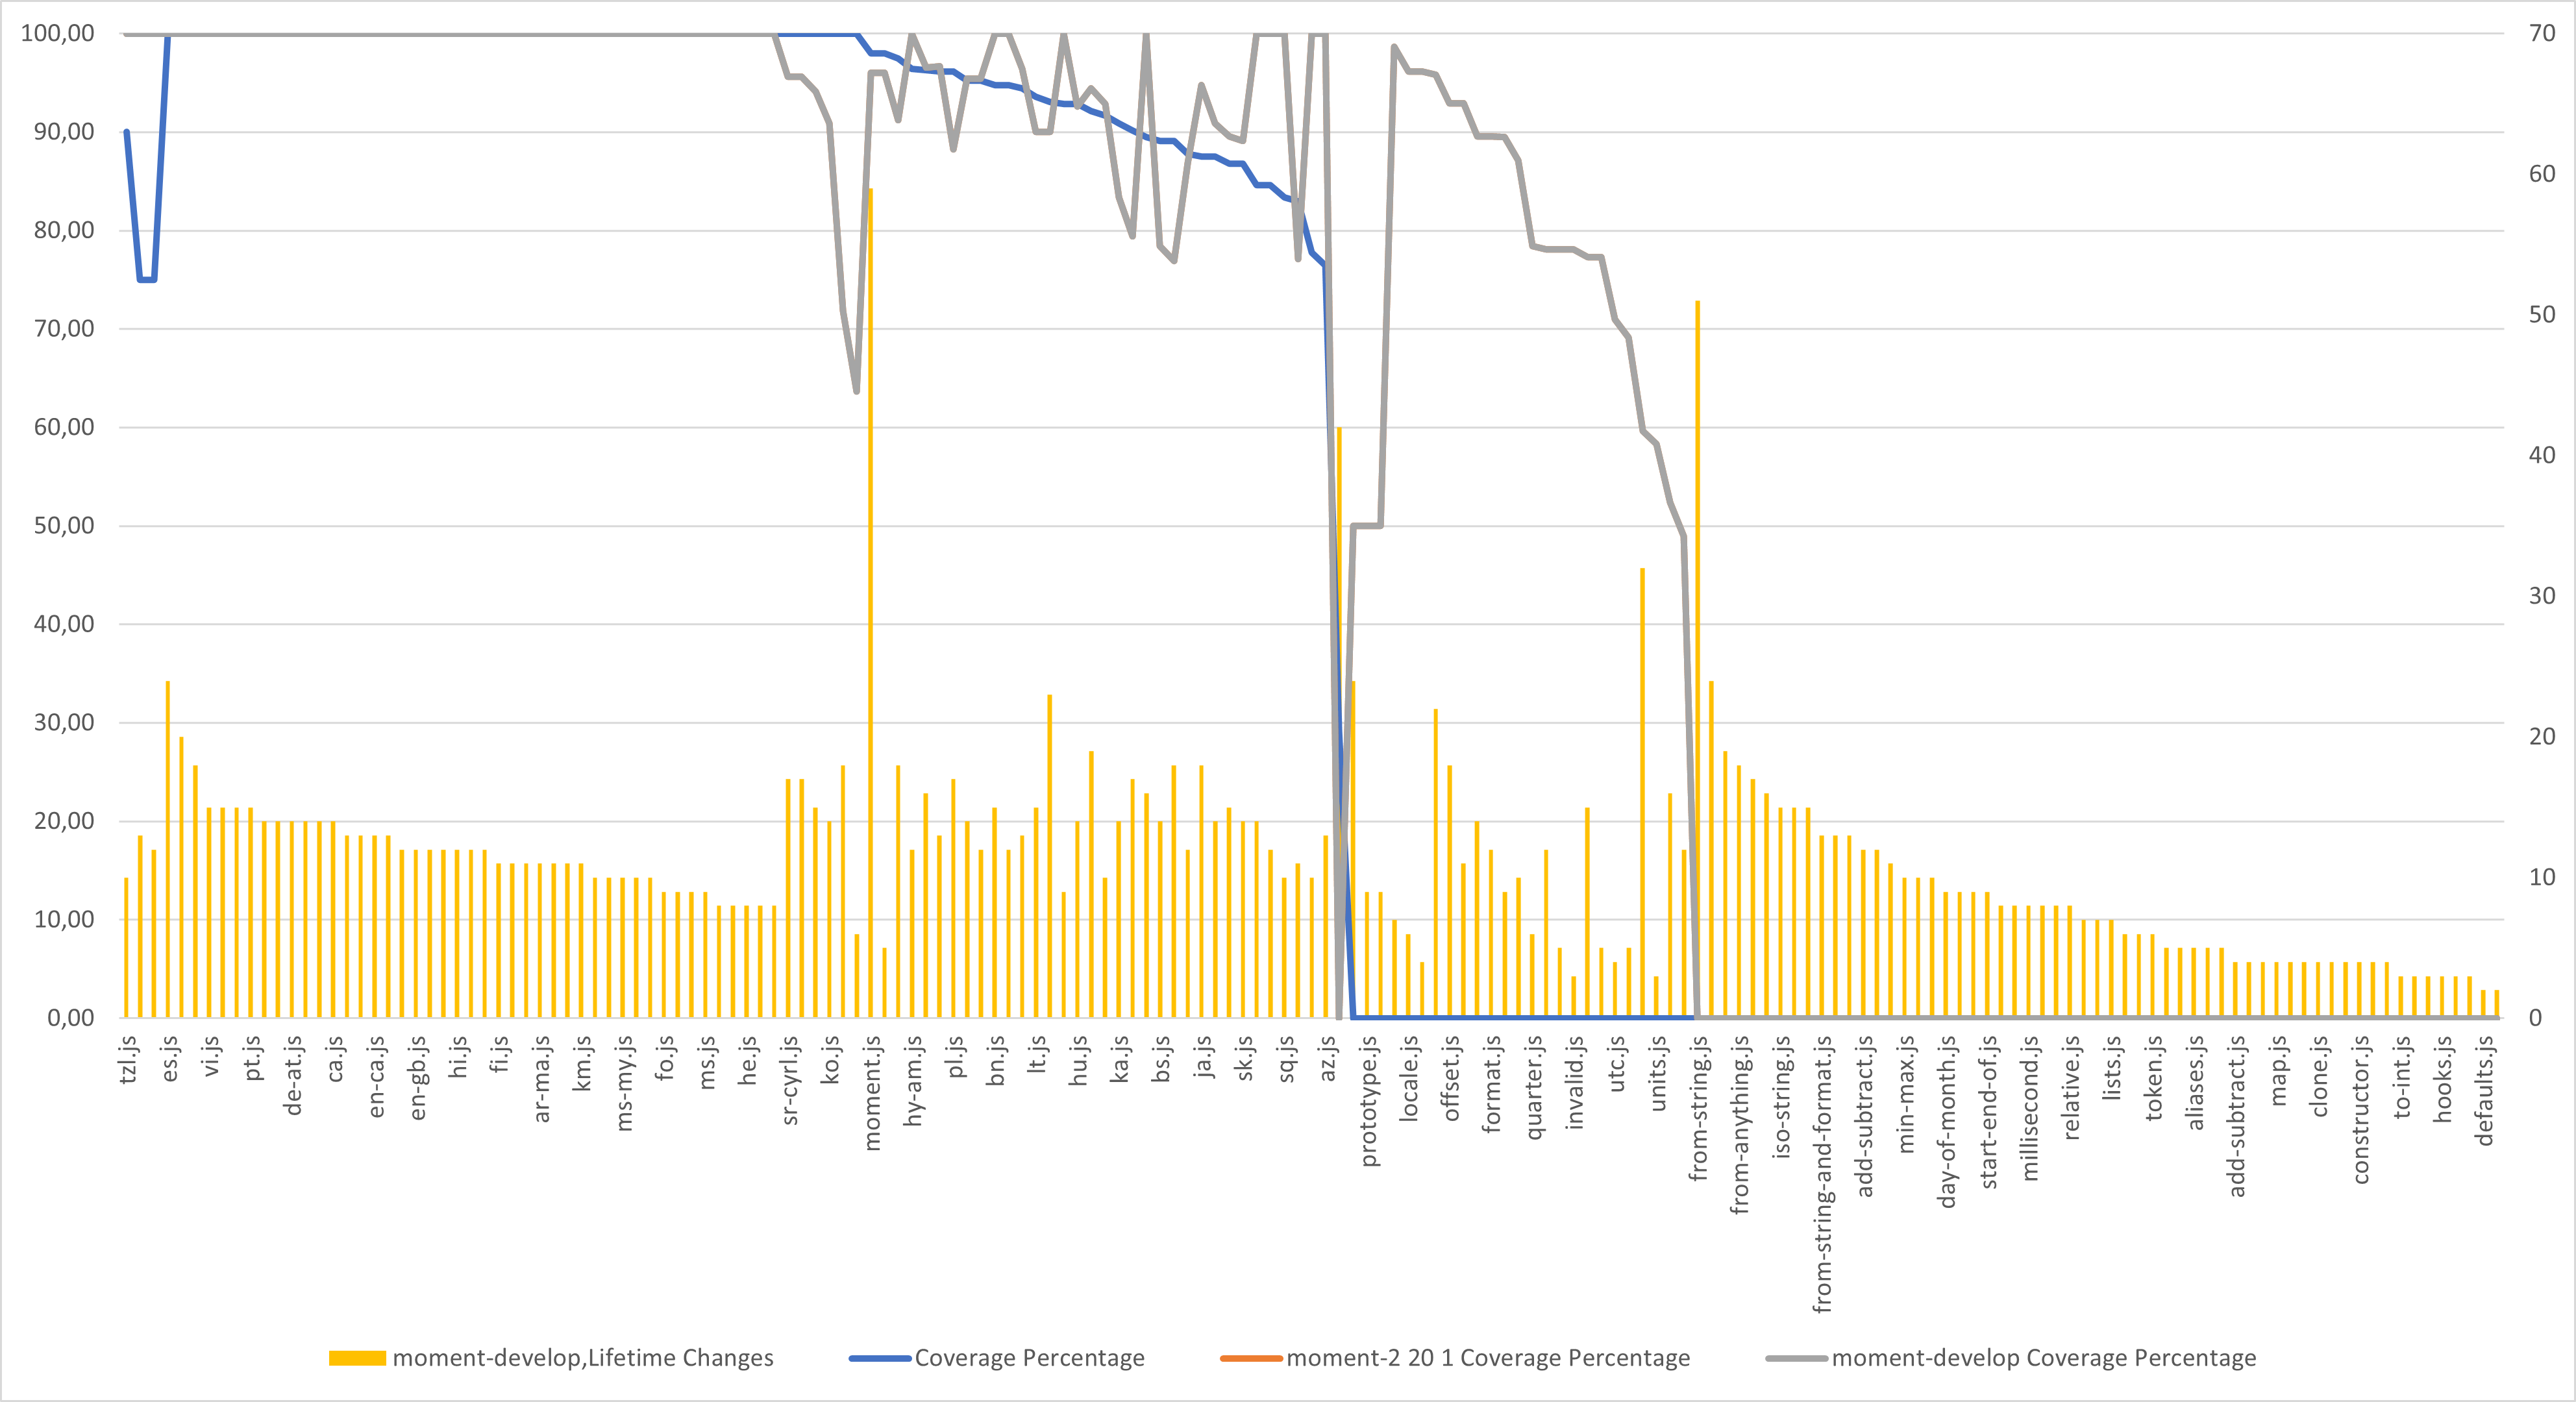
\includegraphics[width=1\textwidth]{images/moment/moment-all-coverage-full.png}
    \caption{Moment.js kódbázisának teljes coverage-e}
    \label{fig:moment-all-coverage-full}
\end{figure}

\section{React}

Utolsóként röviden a React\footnote{https://hu.reactjs.org/} kódbázisára fogunk kitérni. A React a vue-hoz hasonlóan egy webes, JavaScript-alapú frontend könyvtár. A React erősen épít a funkcionális programozásból ismert koncepciókra és a webes világ HTML-CSS-JS szegregációjától eltér a JSX formátumával, ami ezt a hármat ötvözi.

\lstset{language=JavaScript, caption={Egy egyszerű React komponens}}
\begin{lstlisting}
import React, { useState } from 'react';

function Example() {
    return (
        <div>
            <p>You clicked {count} times</p>
            <button onClick={() => setCount(count + 1)}>
                Click me
            </button>
        </div>
    );
}
\end{lstlisting}

Az analízis rövidségének két oka van:
\begin{enumerate}
    \item A react kódbázisa több nagy refactor-on esett át, ami jelentősen megnehezíti a különböző verziók közötti kapcsolatok kialakítását. A snapshot-okat általában a különböző fájlok elérési útvonalain lehet csak összekapcsolni, mert a fájlok nevei nem egyediek, viszont az elérési útvonalak változása miatt csak egy nagyon kis szeletét lehetne megvizsgálni a projektnek
    \item A régebbi react kiadásokra nem lehet coverage report-okat generálni, mert a projekt egyik histórikus függősége egy az egyben el lett távolítva az npm-ről biztonsági okokból
\end{enumerate}

Ennek ellenére a react kódbázisa különösen érdekes lesz, mert egy olyan jelenséget produkál, amit a vue és a moment.js nem.
Elsőként nézzük a React 14-es és 15-ös verziójának a legtöbbet módosított fájljait a \ref{fig:react-14-15-changes} ábrán. Eddig egyelőre nem látszik semmi különös, nagyrészt hasonló értékeket és mintákat látunk, mint a vue és a moment esetében.

\begin{figure}[H]
    \centering
    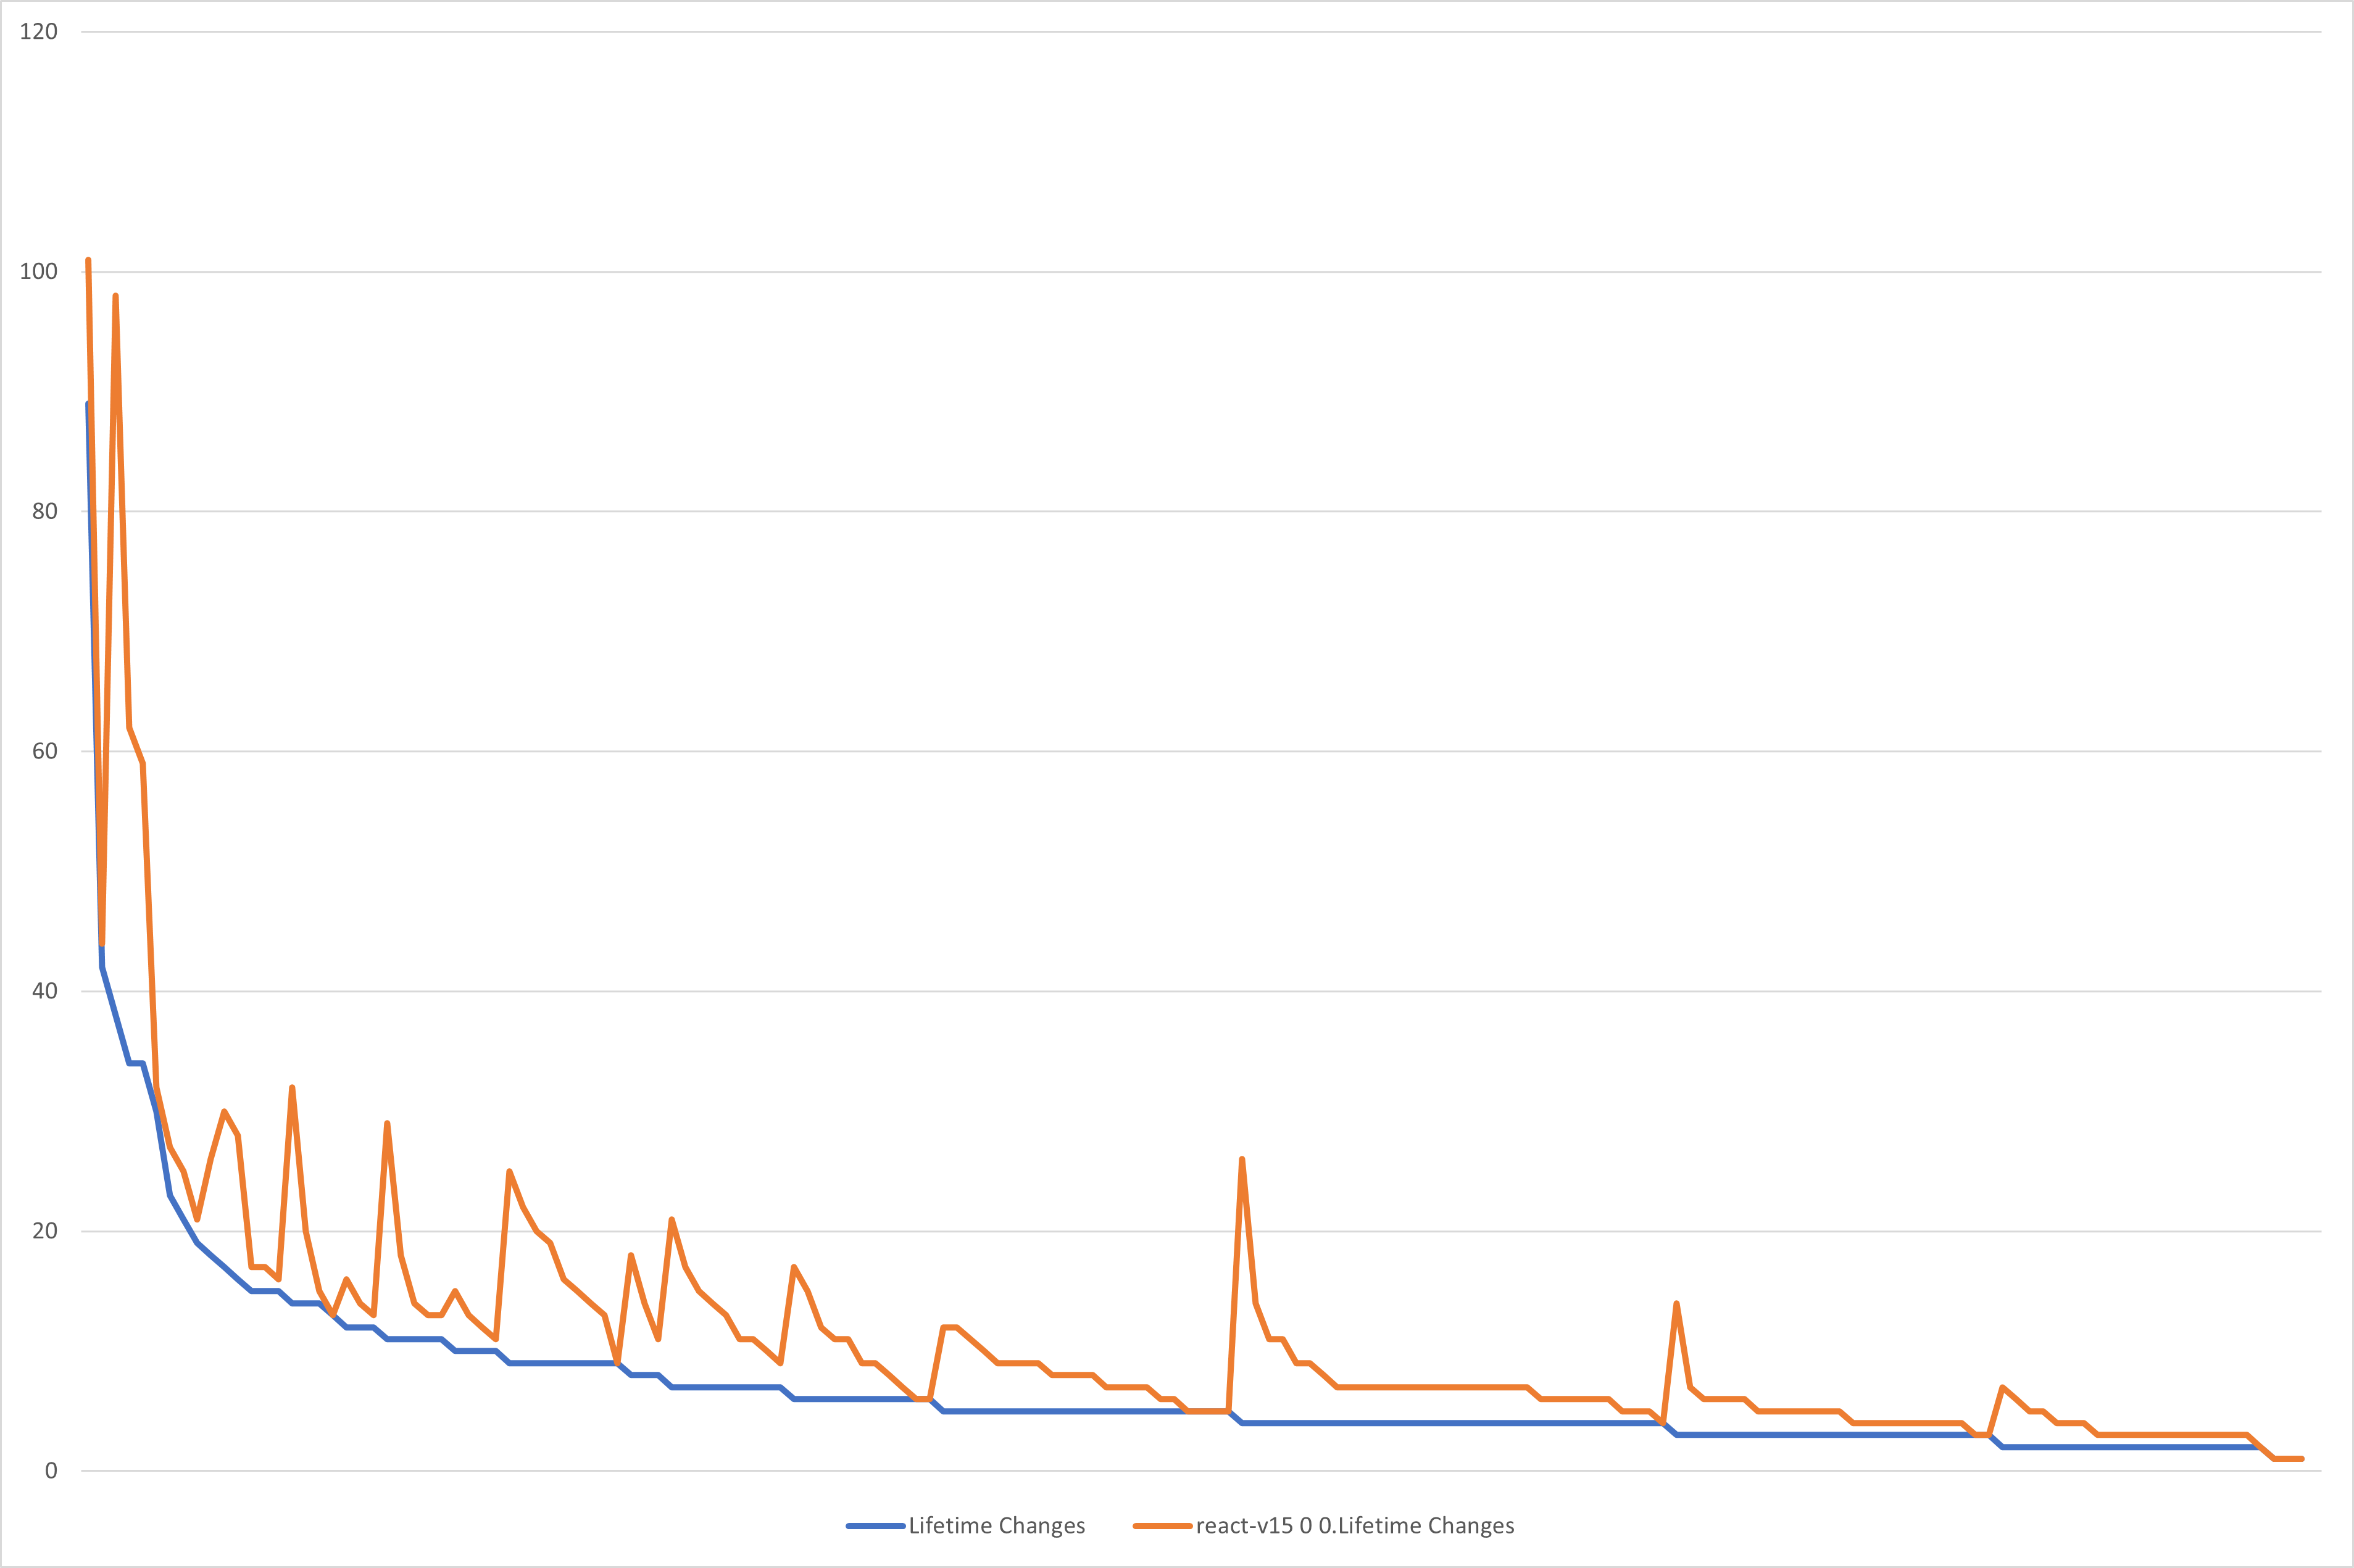
\includegraphics[width=1\textwidth]{images/react/react-14-15-changes.png}
    \caption{A React 14-es és 15-ös verziójának módosítási számai}
    \label{fig:react-14-15-changes}
\end{figure}

Vessünk azonban egy pillantást a \ref{tab:react-all-changes} táblázatra, amiben 16-os verzióban legtöbbet változtatott fájlok szerepelnek a histórikus módosítási adatokkal. Mint látható, a top 10-ben 9 olyan fájl van, amik nem léteztek a 16-os verziót megelőzően. Ez egy kis magyarázatra szorul.

A React a 16-os kiadásban egy teljes új renderelő architektúrára váltott, ami Fiber\footnote{https://reactjs.org/blog/2017/09/26/react-v16.0.html\#new-core-architecture} kódnéven futott. Nyilvánvalóan egy frontend framework legkritikusabb része a DOM rendering, amit gyakorlatilag alapjaitól írtak újra a React fejlesztői. Ugyan ez a változtatás a 16-os verzióban került be az éles kódbázisba, egy párhuzamos branch-en akkor már évek óta aktív fejlesztés alatt állt.

Az eddigi megfigyelések azt mutatták, hogy amikor egy kódbázis elindul egy bizonyos irányba, akkor a korai módosítási minták medrében folyik a fejlesztés a projekt élete során. A react azonban jó példa arra, hogy ez nem feltétlenül igaz: ha a projekt új architektúrára vált, akkor ki lehet kerülni az előre lefektetett mintákat.

Ebben az esetben azonban azonban ez az új architektúra hiába cseréli le a régi, sokat módosított fájlokat, ahogy az \ref{fig:react-all-changes} ábrán látszik a Fiber architektúra pontosan ugyanazt a mintát mutatja, hiába teljesen új kód. Ez természetesen ahogy korábban a code smell-eknél tisztáztuk nem feltétlenül gond, hiszen a projekt korai hibáit javító, új központi architektúra objektíven tud emelni a projekt színvonalán.

\begin{table}[h]
    \centering
    \begin{tabular}{l|l|l|l}
        Filename                    & v14 & v15 & v16 \\ \hline
        ReactFiberScheduler.js      & 0   & 0   & 187 \\
        ReactFiberBeginWork.js      & 0   & 0   & 161 \\
        ReactFiberReconciler.js     & 0   & 0   & 114 \\
        ReactChildFiber.js          & 0   & 0   & 102 \\
        ReactFiberCompleteWork.js   & 0   & 0   & 95  \\
        ReactFiber.js               & 0   & 0   & 87  \\
        ReactFiberCommitWork.js     & 0   & 0   & 78  \\
        ReactDOMFiberComponent.js   & 0   & 0   & 77  \\
        ReactFiberClassComponent.js & 0   & 0   & 73  \\
        ReactCompositeComponent.js  & 34  & 62  & 63  \\
        ReactElement.js             & 17  & 30  & 55  \\
        ReactFiberUpdateQueue.js    & 0   & 0   & 52  \\
        DOMPropertyOperations.js    & 11  & 29  & 49  \\
        ReactElementValidator.js    & 15  & 17  & 49  \\
        HTMLDOMPropertyConfig.js    & 14  & 32  & 48  \\
        ReactFiberContext.js        & 0   & 0   & 44  \\
        ReactDOMComponent.js        & 38  & 38  & 38
    \end{tabular}
    \caption{A React 16-os kiadása}
    \label{tab:react-all-changes}
\end{table}

\begin{figure}[H]
    \centering
    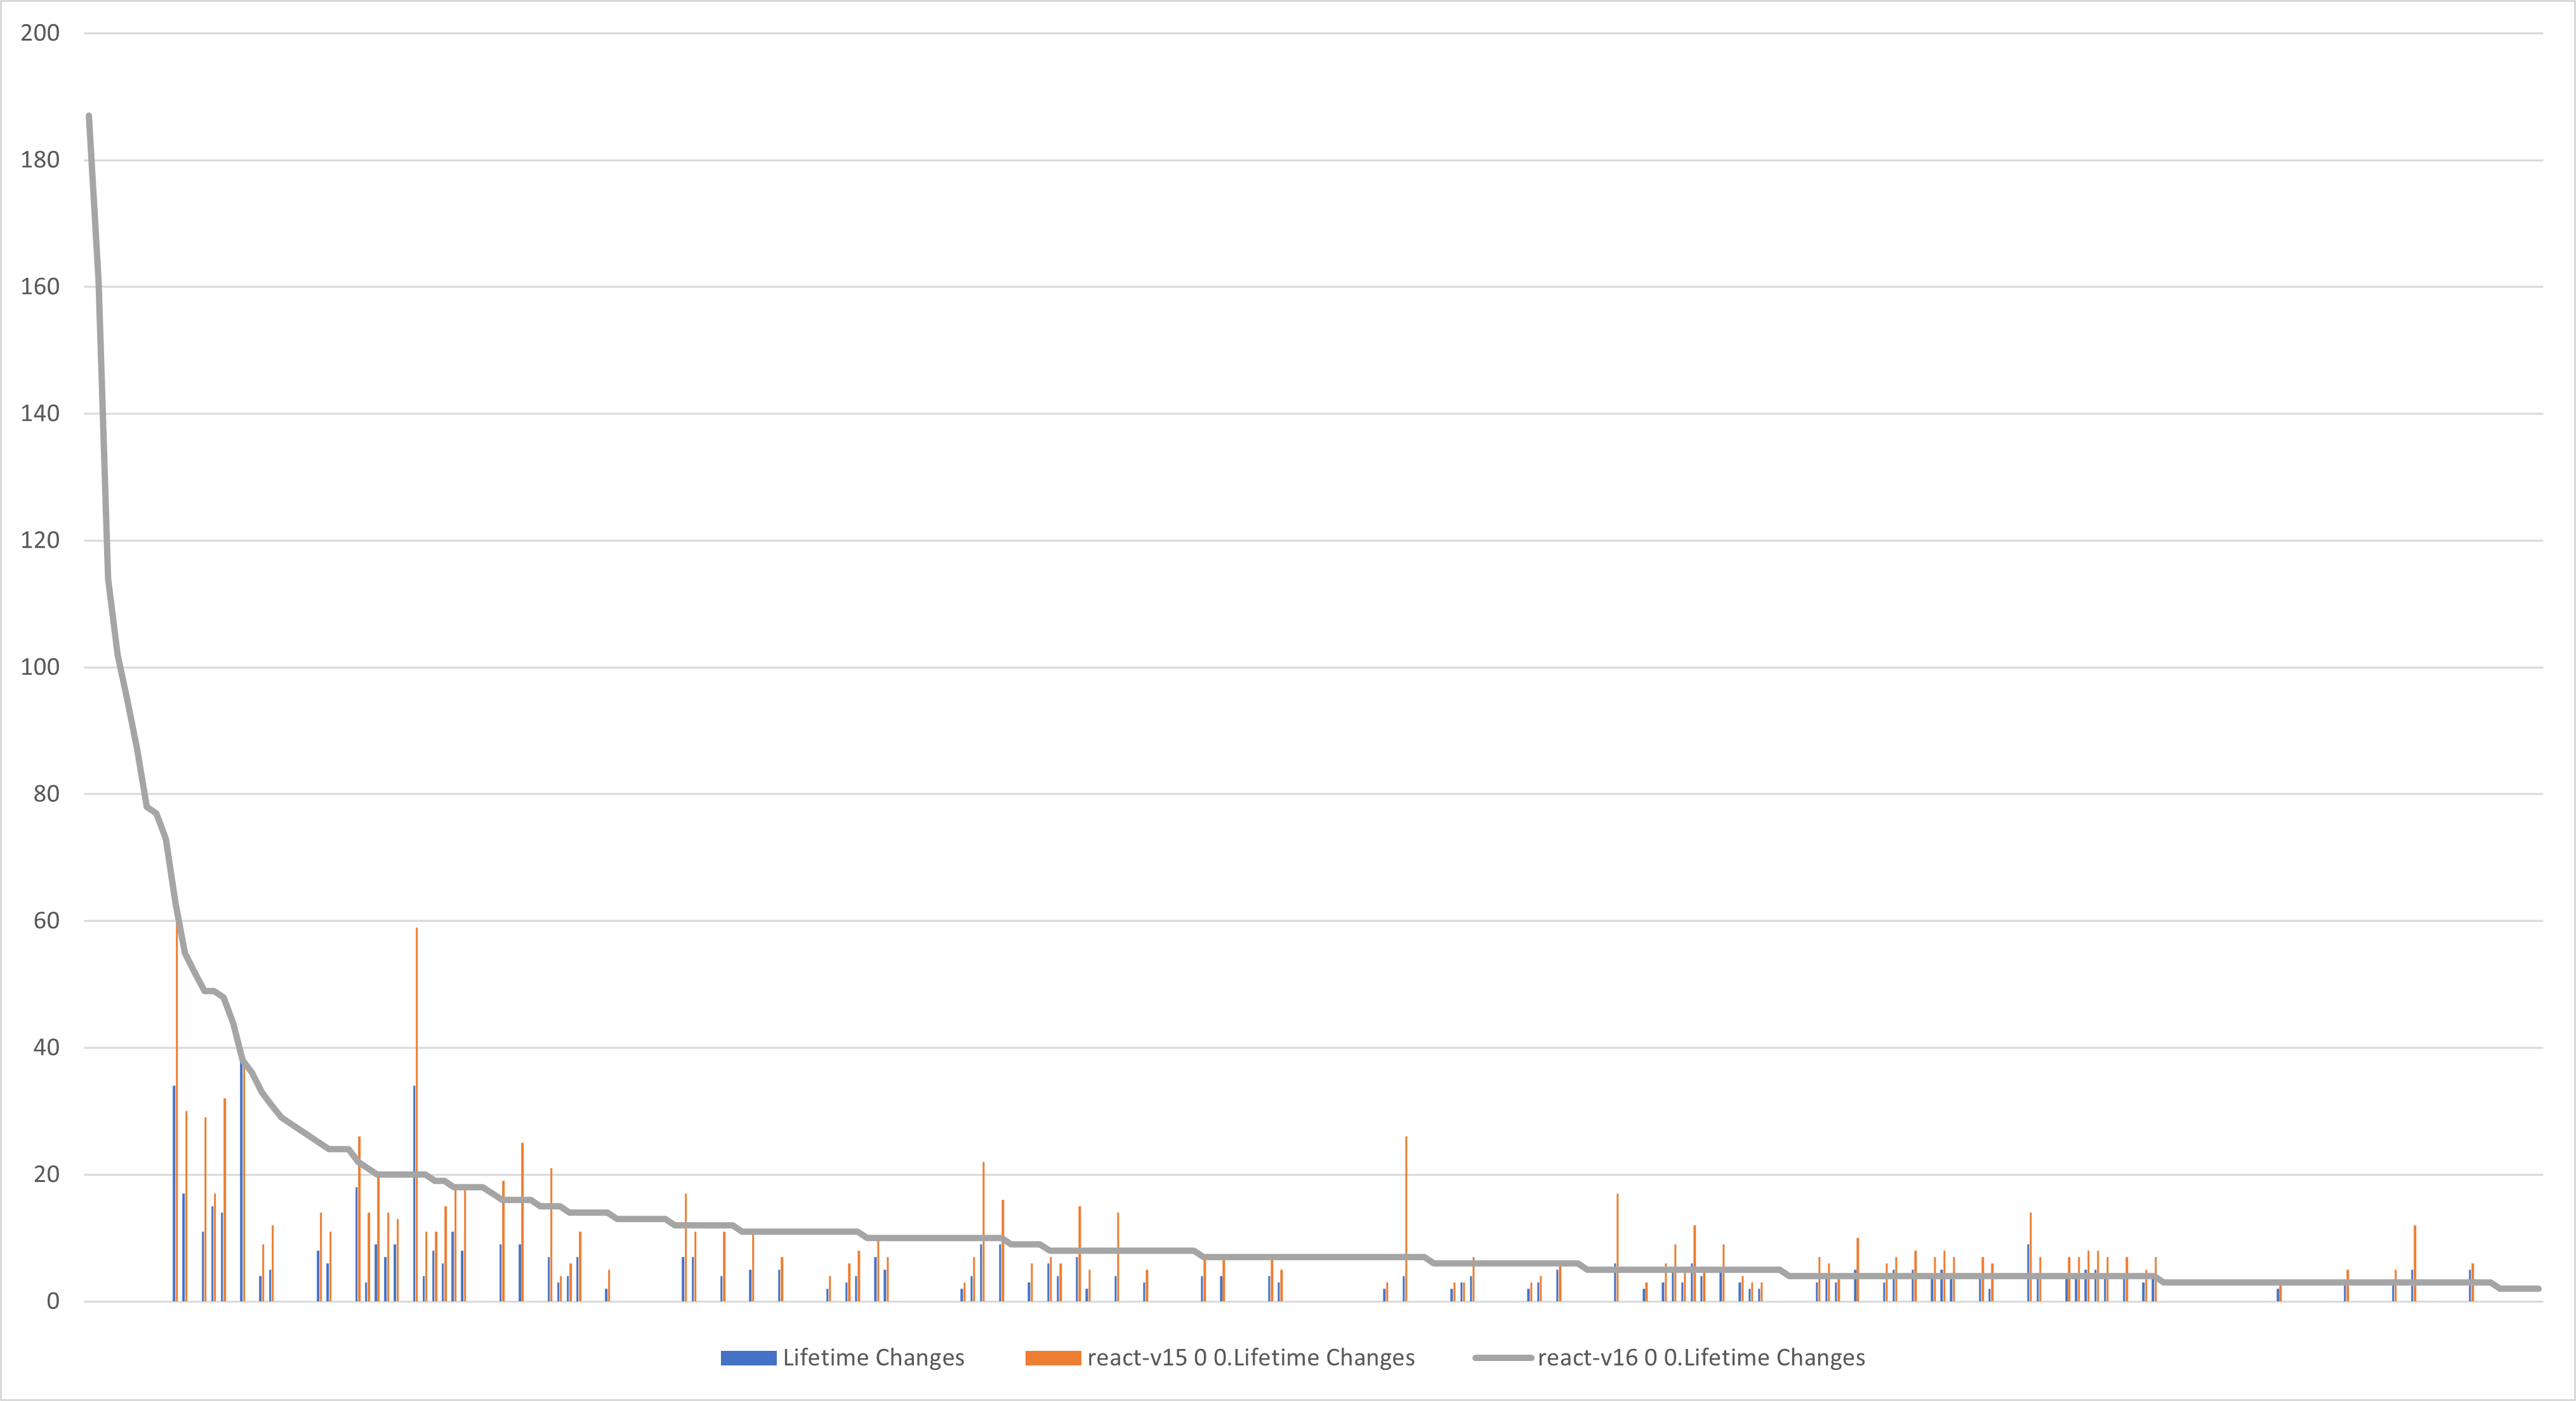
\includegraphics[width=1\textwidth]{images/react/react-all-changes.png}
    \caption{A React teljes kódbázisa a 14-es, 15-ös és 16-os kiadásokban}
    \label{fig:react-all-changes}
\end{figure}